% TODO Sort out the Chapter sections etc.
% The idea is that chapter should only go in a master file, each standalone file should have a section as a tilte so it can be exported as a standalone article
% Master is a book, sub files are articles.
%
% Title stuff needs to go above document class
% so it can be accessed with [titlepage] option
  % this will be on a seperate page though unline \maketitle
\title{Analysis}
\author{Ryan Greenup}
\date{Autumn, 2019}
\documentclass[fleqn, 10pt, titlepage, twoside]{report}
%\twocolumn 
 \usepackage{resources/style}

\begin{document}

%\maketitle
\tableofcontents
\setcounter{tocdepth}{4}
\begin{abstract}
These are the notes that I took in analysis, my working for class tests and working for tutorial problems, the latter two need to be typed it.

I didn't cover anything up to and beyond Complex Series in Churchill's book, that's a shame and definitely something I want to get around to.
\end{abstract}

\part{Lecture Material}

\chapter{Introduction}
\documentclass{article}
\usepackage{./resources/style}
\title{Completeness Property of the Reals}
\begin{document}
	\section{[2.3] Completeness Property of the Reals}
	\subsection{Upper and Lower Bounds [2.3.1]}
	\paragraph{Upper Bound}
	An upper bound is any value greater than or equal to all elements of a set, e.g. $u$ is an upper bound of $A$ if: \\

	\begin{equation}
	  \forall s \in S, \exists u \in \mathbb{R} : u \geq s
	  \label{upperdef}
	\end{equation}


	\paragraph{Lower Bound}
	A lower bound is any value less than or equal to all elements of a set, e.g. $w$ is a lower bound of $A$ if: \\

	\begin{equation}
	  \forall s \in S, \exists w \in \mathbb{R} : w \leq s
	  \label{lowerdef}
	\end{equation}


	\subsection{Supremea and Infima [2.3.2]}
	\paragraph{Supremum}
	The suprema of a set is the smallest upper bound value of some set.\\ 
	This value would be the maximum value of the set if the set had a maximum value.\\
	Let V be the set of all upper bound values, $u$ is a suprema iff:

	\begin{equation}
	  u \leq v, \forall v \in V 
	  \label{supdef}
	\end{equation}

	\paragraph{Infimum}
	The infimum of a set is the largest lower bound value of some set. \\
	This value would be the maximum value of the set if the set had a maximum value.\\
	Let T be the set of all upper bound values, $w$ is a suprema iff:

	\begin{equation}
	  w \leq t, \forall t \in T 
	  \label{infdef}
	\end{equation}

	
\end{document}



\chapter{Sequences and Functions}
\documentclass[class=article, crop=false]{standalone}
\usepackage{./resources/style}
\title{Sequences and their Limits}
\AfterBeginDocument{\tableofcontents}
\begin{document}

\section{Sequences and Their Limits}
A sequence is a type of function that maps from $\mathbb{N} = \left\{ 1, 2, 3, \dots \right\}$
into $\mathbb{R}$\\

Such that the range is contained in some set $S$, e.g. \\
\begin{align}
S = \left\{ 1, \frac{1}{2}, \frac{1}{4}, \frac{1}{8}, \frac{1}{16}, \dots \right\}
  \label{egset1}
\end{align}

In thise case (\ref{egset1}) is a the set of range values of a sequence, this sequence could be described by the function:

\begin{align}
  X : \mathbb{N} \rightarrow \mathbb{R} : x \mapsto \frac{1}{2^{x}}
  \label{eg1asfunc}
\end{align}

\paragraph{Remarks on Sequences}

Unlike a set, a sequence can have repeated elements and the order of elements does matter.\\
Sequences are infinite because they are a function from $\mathbb{N}$ to $\mathbb{R}$.\\
A sequence could be defined to be finite (simply by restricting the domain to an interval or subset of $\mathbb{N}$), however they are defined to be infinite, by nature of their descriptive function, because it is useful to later studies of functions and series (a series is different from a sequence).

\subsection{Notation}
This  (\ref{egset1}) would usually be denoted by the notation:
\begin{equation}
  x_n = \frac{1}{2^{n}} : n \in \mathbb{N}
  \label{notegset}
\end{equation}
However such a sequence can commonly be denoted also:
\begin{align}
  X, \quad  \text{or} \quad  (x_{n}), \quad \text{or} \quad (x_{n} : n \in \mathbb{N})
  \label{altnote}
\end{align}

\paragraph{Ordered Sequences} Ordered Sequences are denoted with parentheses, e.g.
\begin{equation}
  ( (-1)^{n} , n \in \mathbb{N}) = (-1, 1, -1, 1, -1, 1, \dots)
  \label{parordered}
\end{equation}

\paragraph{Unordered Sets} Unordered Sets are denoted with cages/braces and represent the set of range values of a sequence:
\begin{align}
  \left\{ (-1)^n , n \in \mathbb{N} \right\} = \left\{ 1, -1 \right\}
  \label{parunorder}
\end{align}

Be careful because (\ref{parordered}) and (\ref{parunorder}) are different things, one is a sequence of ordered values which could be described by a function, the latter is just the range of such a function.

\subsection{Defining a Sequence}
A sequence can be defined by listing the ordered terms until the rule of formation becomes clear or by specifying the formula, both are correct, so for (\ref{egset1})
\begin{equation}
  X := \left\{ 1, \frac{1}{2}, \frac{1}{4}, \frac{1}{8}, \frac{1}{16}, \dots\right\} = \left\{ 2^{-n} : n \in \mathbb{N} \right\}
  \label{defineseq}
\end{equation}

\subsection{Limits of a sequence}
An informal analogy for the limit of a sequence is:\\

{\small The limit of $x:= \left( x_{n} : n \in \mathbb{N} \right)$ is the expected value of $x_{\infty}$.} \\

\noindent The limit value is usualy denoted $\lim\left( X \right) = \lim\left( x_{n} \right) = x$

\paragraph{The Precise Definition of a Limit} is:

\begin{align}
  \forall \varepsilon > 0, \enspace \exists K : & \notag \\
  & n \geq k \Rightarrow \mid x_{n} - x \mid < \varepsilon 
  \label{precicelimit}
\end{align}

Which says; If for all possible positive values of $\varepsilon$, there is some $k$ value such that if $n \geq K$ then $x_{n}$ is within the $\varepsilon$-neighborhood of the limit value $x$.

%\begin{Theorem}{}{fermat}
%  No three positive integers \(a\), \(b\) and \(c\) satisfy the equation \(a^{n}
%  + b^{n} = c^{n}\) for any integer greater than two.
%\end{Theorem}

\paragraph{Limits are Unique} a sequence will only approach a single limit value.

\paragraph{Equivalent Limit Definitions}
\begin{enumerate}
  \item $X$ converges to $x$ \\
  \item $\forall \varepsilon > 0, \enspace \exists K : n\geq K \Rightarrow \mid x_{n} - x \mid < \varepsilon$
  \item $\forall \varepsilon > 0, \enspace \exists K : n\geq K \Rightarrow \left( x- \varepsilon \right) < x_{n} < \left( x + \varepsilon \right)$
  \item for every $\varepsilon$-neighborhood $V_{\varepsilon}\left( x \right)$, there exists some $K \in \mathbb{N}$:
    \subitem $\forall n \geq K, \enspace x_{n} \in V_{\varepsilon}\left( x \right)$
\end{enumerate}

\paragraph{The Tail of a Sequence [ 3.1.9]} or the $m$-tail of a sequence is the sequence starting from the $m^{\text{th}}$ term, a tail will aproach the same limit as the original sequence because they will both have the same expected value for $x_{\infty}$


\section{[3.2] Limit Theorems}
\subsection{Intervals [2.5]}

An \textbf{Open Interval} is defined:

\begin{align}
  \left( a,b \right) := \left\{ x \in \mathbb{R} : a<x<b \right\}
  \label{openintdef}
\end{align}

A \textbf{Closed Interval} is defined:

\begin{align}
  \left[ a,b \right] := \left\{ x \in \mathbb{R} : a\leq x\leq b \right\}
  \label{closedintdef}
\end{align}

\subsection{Bounded Sequences [3.2.1]}

If $x_{n} \in \left[ -M, M \right]$, for some real positive $M$,  then $x_{n}$ is said to be bounded. \\

{\small i.e. if the set of range values of a sequence $\left\{ x_{n} : n \in \mathbb{N} \right\}$ is a bounded set then the sequence is said to be a bounded sequence}

\paragraph{Bounded Subsets [2.3.1]} are subsets of the real numbers that have a maximum and a minimum, Take for example:
\begin{align}
  \left\{ 1, 2, 3, 4, \dots 25, 50, 53, 54  \right\}
  \label{boundedeg} \\
  \left\{ p : p = 2n, n \in \mathbb{Z^+} \right\} 
  \label{notbounded}
\end{align}
In the example above (\ref{boundedeg}) is bounded because the minimum is 1 and the maximum value is 54, also notice that (\ref{boundedeg}) is not a continuous subset of $\mathbb{R}$, it jumps from 25 to 50 and it doesn't include any quotient values, it is still however a bounded subset of $\mathbb{R}$. 

However (\ref{notbounded}) is not a bounded subset because it does not have an upper bound value, it does have a lower bound, anything less than 1, but that means it is only bounded below and it is not a bounded subset of $\mathbb{R}$.

\paragraph{Bounded Subsets and Convergence [3.2.2]} If a subset is Convergent it must be bounded because it has a starting value and it approaches another value, e.g.

\begin{align}
  \left\{ 1, \sfrac{1}{2}, \sfrac{1}{4}, \sfrac{1}{8}, \sfrac{1}{16}, \sfrac{1}{32} \dots  \right\}  
  \label{boundconeg}
\end{align}

This set (\ref{boundconeg}) converges to 0 and starts from 1, so it must have an upper bound of 1\\ (because all $x_{n} \leq 1$, $x_n \geq 0$ (\small it is $\leq/\geq$ not $</>$)

  If a subset is bounded however it doesn't necessarily need to be convergent, e.g.:

  \begin{align}
    \left( 1,2,1,2,1,2,1, \dots \right)
    \label{unboundconeg}
  \end{align}

  This set (\ref{unboundconeg}) does not converge but is clearly bounded by 1 and 2, {\footnotesize \\
    (however a monotone series that is bounded will converge but that's in [3.3])
}

%{\small basically if a sequence converges it must be possible to find a maximum and minimum value in the sequence even though the sequence isn't necessarily finite, if it is possible to find a maximum and minimum value then those two values are also upper and lower bounds respectively.

%  This can be explained in terms of neighbourhoods as well, take some neighbourhood of the limit value $x$, there could very well be infinite terms within that neighbourhood but there must be finite terms outside that neighbourhood (because a sequence must have a starting value), the values outside the neigborhood are finite and finite sets must be bounded, the sets inside the neighbourhood are bounded by the neighborhood and hence the entire sequence of values is bounded.


\paragraph{Arithmetic with Sequences}
In order to manipulate sequences we will define operations that relate to addition and multiplication, this is by definition simply so we can use them. \\

Let,

\begin{align}
  X = (x_n) \quad Y = (y_n) \quad Z = (z_n)
  \label{seqdefgen}
\end{align}

We define the following Operations [3.2, p. 63]:

\begin{align}
  X+Y &= \left( x_{n} + y_{n} \right) \label{addseqdef} \\
  X-Y &= \left( x_{n} - y_{n} \right) \label{minseqdef} \\ 
  c \cdot X &= \left( c\cdot x_{n}\right) \label{conmultseqdef}\\
  X\times Y &= \left( x_{n} \times y_{n} \right) \label{multseqdef} \\
  X/Y &= \left( x_{n} \div y_{n} \right) 
  \label{divseqdef}
\end{align}


%\begin{tabular}{<{$}l>{$}l<{$}@{}}
 %Sequence Addition            &   X+Y = \left( x_{n} + y_{n} \right) \\
 %Sequence Subtraction &   X-Y = \left( x_{n} - y_{n} \right) \\
 %Sequence Constant Mult. &   c \cdot X = \left( c\cdot x_{n}\right) \\
 %Sequence Multiplicaiton &   X\times Y = \left( x_{n} \times  y_{n} \right) \\
 %Sequence Division &   X / Y = \left( x_{n} \div y_{n} \right) \\
 %\end{tabular}



\subparagraph{Limits of Sequences for Arithmetic with Sequences [3.2.3]}
Because the limit of a sequence is essentially the expected value of $x_{\infty}$ it stands to reason that the limit will distribute over the basic operations: \\

Let,

\begin{align}
  \lim X = \lim(x_n) =  x \quad \lim Y = \lim(y_n) = y \quad \lim Z = \lim(z_n) = z
  \label{seqdeflim}
\end{align}

Then the limits are:

\begin{alignat}{2}
  \lim  \left( X+Y \right) &= \lim X + \lim Y &= x + y
  \label{addlimdef} \\
  \lim  \left( X-Y \right) &= \lim X - \lim Y &= x - y 
  \label{minlimdef} \\
  \lim  \left( c \cdot X \right) &= c \cdot \lim X  &= c \cdot x
  \label{conmultlimdef} \\
  \lim  \left( X\times Y \right) &= \lim X \times \lim Y &= x \times y
  \label{multlimdef} \\
  \lim  \left( X/Y \right) &= \lim X \div \lim Y &= \sfrac{x}{y} 
  \label{divlimdef}
\end{alignat}


%\begin{tabular}{@{}>{$}l<{$}l>{$}l<{$}@{}}
%m   & módulo            & m\textgreater 0\\
%a   & multiplicador     & 0\textless a\textless m\\ c   & constante aditiva & 0\leq c<m\\
%x_0 & valor inicial     & 0\leq x_0 <m
%\end{tabular}





\subsection{Limit Theorems}
The rest of the chapter provides values of limits, it begins with this simple property of sequence limits:
\begin{align}
  &\text{\textbf{If} $X$ is convergent (i.e. a limit exists) and all $x_n\geq 0$}  \notag \\
  &\text{\textbf{Then} $\lim\left( x_{n} \right)\geq 0$} \tag{3.2.4}
  \label{324}
\end{align}

We can build on this theorem by generalising it a little bit:


\begin{align}
  &\text{\textbf{If} $X$ and $Y$ are convergent (i.e. limits exists) and all $x_n\leq y_n$}  \notag \\
  &\text{\textbf{Then} $\lim\left( x_{n} \right)\leq \lim \left( y_n \right)$} \tag{3.2.5}
  \label{325}
\end{align}

  If a sequence has a limit and exists within in an interval, then the limit is also within that interval.


\begin{align}
  &\text{\textbf{If} $X$ is convergent (i.e. a limit exists) and all $x_n \in \left[ a,b \right]$}  \notag \\
  &\text{\textbf{Then} $\lim\left( x_{n} \right) \in \left[ a,b \right]$} \tag{3.2.6}
  \label{326}
\end{align}

\paragraph{Squeeze Theorem} Now if a sequence is always between two other sequences and those sequences have the same limit, then the original sequence must share that limit. 


\begin{align}
  &\text{\textbf{If} $X, Y, Z$ are convergent (i.e. limits exist) and all $\left( x_n \right) \leq \left( y_n \right) \leq \left( z_n \right)$ and $\lim X = \lim Z$} \notag \\
  &\text{\textbf{Then} $\lim X = \lim Y = \lim Z$} \tag{3.2.7}
  \label{327}
\end{align}

\paragraph{Limits Sequence Functions} I'd be careful here because the textbook doesn't necessarily imply that all functions will demonstrate this behaviour:

\begin{align}
  \lvert \lim (x_n) \rvert = \lim \left( \lvert x_n \rvert \right) \tag{3.2.9}
  \label{329} \\
  \left( \sqrt{\lim \left( x_n \right)} \right) = \lim \left( \sqrt{x_n} \right) \tag{3.2.10} \label{3210}
\end{align}

\paragraph{Ratios}

The next theorem is useful where a ratio of the next and preceeding term can be reduced into a form that must be less than one $\left( \frac{x_{n+1}}{x_n} < 1 \right)$.\\


\begin{align}
&  \text{\textbf{If} all $(x_n) > 0$ and $L := \lim \left( \frac{x_{n+1}}{x_n} \right)$ exists} \notag \\
& \text{\textbf{Then} $L<1 \implies \lim X = 0$} \tag{3.2.11} \label{3211}
%&    \text{\textbf{If} $L < 1$} \\
%  &\text{\textbf{Then} $\lim X = 0$} \tag{3.2.11}
%  \label{3211}
\end{align}


\section{[3.3] Monotone Sequences}
A monotone sequence is a sequence that is either increasing or decreasing, where:\\
\ \\
$X = (x_n)$ is said to be \textbf{decreasing} if:
\begin{align}
  x_n \geq x_{n+1}, \enspace  \forall n \in \mathbb{N}
  \label{331dec}
\end{align}

\noindent $X= (x_n)$ is said to be \textbf{increasing} if:
\begin{align}
  x_n \leq x_{n+1}, \enspace  \forall n \in \mathbb{N}
  \label{331inc}
\end{align}

\subsection{Monotone Convergence Theorem [3.3.2]}
A monotone sequence  $\left( x_n \right)$ is convergent $\iff$ it is bounded. {\tiny $\left( \left\{ x_n \right\} \in \mathbb{R} \right)$}

{\footnotesize  Whereas an ordinary set is convergent $\implies$ Bounded (at 3.2.2)} \\

Furthermore,
\begin{enumerate}
\item If $X = (x_n)$ is \textit{bounded} and \textit{increasing}, then:
  \begin{align}
    \lim (x_n) = \sup \left\{ x_n : n \in \mathbb{N} \right\}
    \label{mctboundconinc}
  \end{align}

\item If $Y = (y_n)$ is \textit{bounded} and \textit{decreasing} then:
  \begin{align}
    \lim (y_n) = \inf \left\{ y_n : n \in \mathbb{N} \right\}
    \label{mctboundcondec}
  \end{align}
\end{enumerate}

\paragraph{Why this is Important} The \textit{Monotone Convergence Theorem} is important because it:

\begin{enumerate}
  \item Guarantees a Limit exists for a bounded Monotone Sequence
  \item Gives us a way to solve that limit if we can evaluate the supremum/infimum
    \subitem Supremum and Infimum are defined at [2.3.1]-[2.3.2]
\end{enumerate}

\paragraph{Example Application}
\subparagraph{Deductive Sequence}
Evaluate $\lim\left( \sfrac{1}{\sqrt{n}} \right)$ \\
Observe that the corresponding sequence is $(x_n) = \left( x : x = \frac{1}{\sqrt{n}}, n \in \mathbb{N} \right)$ \\
\ \\
The set of range values would be $\left\{ x_n \right\} = \left\{ 1, \frac{1}{\sqrt{2}}, \frac{1}{\sqrt{3}}, \frac{1}{2}, \dots \right\} \in [1, 0)$ \\
\ \\
The Infimum (i.e. the largest value smaller than all $x_n$) of $x_n$ is 0, so the \textit{Monotone Convergence Theorem} provides  $\lim (x_n) = 0$

\begin{flushright}
  $\blacksquare$
\end{flushright}

\subparagraph{Inductive Sequence} Evaluate $x_{1} = 2, \enspace x_{n+1} = 2 + \frac{1}{x_n}$ \\
Let the limit be:
\begin{align}
  \lim (x_n) = x
  \label{limdefindeg}
\end{align}

We know that the limit must be equal to the limit of the $m$-tail of the sequence by [3.1.9], so:
\begin{align}
  \lim(x_n) = x&=\lim(x_{n+1})
  \label{limdefegind} \\
  &= \lim\left( 2+ \frac{1}{x_n} \right)  \notag \\
  &= \lim \left( 2 \right) + \lim \left( \frac{1}{x_n} \right)  \notag && \text{Justified by (3.2.3)}\\
  \intertext{This step is allowable if and only if $x_n \neq 0$, which means $x_n > 0$, hence it is now known that $\lim(x_n) > 0$ by (3.2.4) } \\
  &= 2 + \frac{\lim{(1)}}{\lim{(x_n)}}  \notag  \\
  \implies x&= 2 + \frac{1}{x} \notag \\
  \implies  0 &= x^{2} -2x - 1 && x>0  \notag \\
  \implies x &= 1 \pm \sqrt{2} \enspace  \wedge \enspace x>0  \notag \\
  \implies x &= 1 + \sqrt{2}  \notag  
\end{align}

\paragraph{Solving Roots with the \textit{Monotone Convergence Theorem}[3.3.5]}
This can be used to solve square roots, it's laid out in a very convoluted fashion in the text book.
\paragraph{Euler's Number}
Euler's number is the number $e = \lim(e_{n}): \enspace e_{n} = \left( 1 + \frac{1}{n} \right)^n$

\begin{flushright}
  $\blacksquare$
\end{flushright}

\section{[3.4] Subsequences}
This section [3.4] is all about subsequences, and how they interact with convergence, it also introduces the limit superior/inferior.

\subsection{Subsequences [3.4.1]}
Let $X = \left( x_n \right)$ be a sequence of real numbers, from left to right pick values of $X$ (e.g. every third value or perhaps the 2nd, 3rd, 5th, 7th, 11th etc), these values also form a sequence and that sequence is a subsequence of $X$. \\

Formally, a subsequence $X'$ of $X$ is a sequence, composed of elements of $(x_n)$, where $n_1 < n_2 < n_3 \dots \in \mathbb{N}$:

\begin{align}
  \left( x_{n_1}, x_{n_2}, x_{n_3}, \dots \right)
  \label{341} \tag{3.4.1}
\end{align}


\paragraph{Convergence of Subsequences} If a sequence converges to some value $x=\lim X$, then the subsequence must also converge to that value (because a subsequence preserves the order of the original sequence).

\paragraph{Non-Converging Subsequences [3.4.4]} The following are equivalent statements:

\begin{enumerate}
  \item The sequence $X=(x_n)$ does not converge to $x \in \mathbb{R}$
  \item There exists some value $\varepsilon_0$, such that for any $k \in \mathbb{N}$, there exists $n_k\in \mathbb{N}$ such that $n\geq k$ and $\lvert x_{n_k} - x \rvert \geq \varepsilon_0$
  \item There exists an $\varepsilon_0 > 0$ and a subsequence $X' = \left( x_{n_{k}} \right)$ of $X$ such that $\lvert x_{n_k} - x \rvert \geq \varepsilon_0$ for all $k \in \mathbb{N}$ 
\end{enumerate}

\paragraph{Divergence Criteria [3.4.5]}
If either of the following properties is satisfied, a sequence $X$ can be shown to be divergent.

\begin{enumerate}
  \item $X$ has two convergent subsequences that converge to different limits
    \subitem because there can only be one limit for a subsequence
  \item $X$ is unbounded
    \subitem If $X$ was convergent it would be necessarily bound by the starting and limit value.
\end{enumerate}

\subsection{Existence of Monotone Subsequences [3.4.7]}
If $X = \left( x_n \right)$ is a sequence of real numbers, then there is a subsequence of $X$ that is monotone. \\
Basically all this says is it is possible to pick values from $X$ in order so that they either increase or decrease (recall that the definition of increasing allows being equal to the previous value by (\ref{331dec})).


\subsection{[3.4.8] The Bolzana-Weierstrass Theorem [3.4.8]}
This is Italian-German, so it's pronounced (bolt-tza-no)-(vai-ya-strahzz). \\
\ \\
If a sequence is bounded then all subsequences are bounded (this is by definition (3.4.1)),\\ A monotone subsequence is guaranteed to exist by (3.4.7),\\ A bounded monotone subsequence must converge by the \textit{MCT} (3.3.2),\\ Hence a convergent subsequence must exist.\\ 
\ \\ That's the Theorem: \textit{A bounded subsequence must always have a convergent subsequence}


\subsection{Upper and Lower Bounds [2.3.1]}
\paragraph{Upper Bound}
An upper bound is any value greater than or equal to all elements of a set, e.g. $u$ is an upper bound of $A$ if: \\

\begin{equation}
  \forall s \in S, \exists u \in \mathbb{R} : u \geq s
  \label{upperdef}
\end{equation}


\paragraph{Lower Bound}
A lower bound is any value less than or equal to all elements of a set, e.g. $w$ is a lower bound of $A$ if: \\

 \begin{equation}
 \forall s \in S, \exists w \in \mathbb{R} : w \leq s
 \label{lowerdef}
\end{equation}


\subsection{Supremum and Infima [2.3.2]}
\paragraph{Supremum}
The suprema of a set is the smallest upper bound value of some set.\\ 
This value would be the maximum value of the set if the set had a maximum value.\\
Let V be the set of all upper bound values, $u$ is a suprema iff:

\begin{equation}
 u \leq v, \forall v \in V 
 \label{supdef}
\end{equation}

So if a set has a maximum value, the supremum is the maximum value of the set:
\begin{align}
  \exists \max\left\{ \left( x_n \right) \right\} \implies \max(x_n) = \sup \left\{ x_n \right\}
  \label{maxassup}
\end{align}
If the set doesn't have a maximum, then the supremum is the next largest value, e.g.\\
$\sup \left( 3, 5 \right) = 5$ and $\sup \left[ 3, 5 \right] = 5 = \max \left( \left[ 3, 5 \right] \right)$  

\paragraph{Infimum}
The infimum of a set is the largest lower bound value of some set. \\
This value would be the maximum value of the set if the set had a maximum value.\\
Let T be the set of all upper bound values, $w$ is a suprema iff:

\begin{equation}
  w \leq t, \forall t \in T 
  \label{infdef}
\end{equation}

So if a set has a minimum value, the infimum is the minimum value of the set:
\begin{align}
  \exists \min\left\{ \left( x_n \right) \right\} \implies \min(x_n) = \inf \left\{ x_n \right\}
  \label{minassup}
\end{align}
If the set doesn't have a minimum, then the infimum is the next largest value, e.g.\\
$\inf \left( 3, 5 \right) = 3$ and $\inf \left[ 3, 5 \right] = 3 = \min \left( \left[ 3, 5 \right] \right)$  

\subsection{Limit Superior and Limit Inferior [3.4.10]}
So the textbook wasn't particularly helpful, instead this video by \textit{SplineGuyMath}\footnote{https://www.youtube.com/watch?v=khypO8MQpdc} was really good

\paragraph{Summary}
Sometimes it is useful to know the smallest and largest limits that subsequences can have. For this the limit inferior and limit superior are used.
\subparagraph{Limit Inferior}
The Limit Inferior is the smallest limit that any subsequence of $x_n$ can have; it is denoted:

\begin{align}
  \limsup \left( X \right) = \limsup \left( x_n \right) = \varlimsup \left( x_n \right) %use \limsup not \lim \sup because limits underneath will line up better
  \label{limsupnotdef}
\end{align}
\subparagraph{Limit Superior} 
The limit superior is the largest limit that ay subsequence of $x_n$ can have; it is denoted:

\begin{align}
  \liminf \left( X \right) = \liminf \left( x_n \right) = \varliminf \left( x_n \right) %use \liminf not \lim \sup because limits underneath will line up better
  \label{liminfnotdef}
\end{align}

\paragraph{Definition}
\subparagraph{Limit Superior} \ \\
Let $X = x_{n}$ be bounded above, and  \\
$M_n = \sup \left\{ x_n, x_{n+1}, x_{n+2}, \dots \right\} \qquad \qquad$ (This is the $\left( n-1 \right)$ tail of $x_n$) \\
Then the limit superior of $x_n$ is:
\begin{align}
  \lim \sup \left\{ X \right\} = \lim \sup \left\{ x_n \right\} = \lim \left\{ M_n \right\}
  \label{limsupdef}
\end{align}

This definition of a limit superior works because subsequences preserve order, so if the maximum value of a sequence approaches a limit as we move along that sequence (i.e. take tails), that limit must be the largest of all limits of possible subsequences.

\subparagraph{Limit Inferior} \ \\
Let $X = x_{n}$ be bounded below, and  \\
$m_n = \inf \left\{ x_n, x_{n+1}, x_{n+2}, \dots \right\} \qquad \qquad$ (This is the $\left( n-1 \right)$ tail of $x_n$) \\
Then the limit inferior of $x_n$ is:
\begin{align}
  \lim \inf \left\{ X \right\} = \lim \inf \left\{ x_n \right\} = \lim \left\{ m_n \right\}
  \label{liminfdef}
\end{align}

This definition of a limit inferior works because subsequences preserve order, so if the minimum value of a sequence approaches a limit as we move along that sequence (i.e. take tails), that limit must be the smallest of all limits of possible subsequences.


\subparagraph{Example} 
Find the limit superior and limit inferior  of:
\begin{align}
  B = \left( b_n \right) = \left( 1+\frac{1}{2^n} \right) = \left( \frac{3}{2}, \frac{5}{4}, \frac{9}{8}, \frac{17}{16}, \dots \right)
  \label{eglimb}
\end{align}

First consider the value of $M_n$:

\begin{align}
  M_n & = \sup \left\{ b_n, b_{n+1}, b_{n+2}, \dots \right\} \label{Mnvalinsupeg}\\
  &= \left( 1.5, 1.25, 1.0625, 1.03125, 10.015625, \dots \right) \label{supsasdec} \\
  \lim(M_n) &= 1 \label{Mnis1supeg} \\
  \lim \sup (M_n) &= 1 \label{equivtolimsup}
\end{align}


Now consider the value of $m_n$:

\begin{align}
  m_n & = \inf\left\{ b_n, b_{n+1}, b_{n+2}, \dots \right\} \label{mnvalininfeg}\\
  &= \left( 0, 0, 0, 0, 0, \dots \right) \label{infvals} \\
  \lim(m_n) &= 0 \label{mnis1infeg} \\
  \lim \inf (M_n) &= 0 \label{equivtoliminf}
\end{align}

Hence the largest limit that any subsequence of $\left( b_n \right)$ can have (i.e. the \textbf{Limit Superior}) is 1 and
the smallest limit that any subsequence of $\left( b_n \right)$ can have (i.e. the \textbf{Limit Inferior}) is 0.

\paragraph{Convergent Sequences and limit Superior/Inferior [3.4.12]}
 If a sequence is bounded it must have a limit superior and a limit inferior, if it is convergent then:
 \begin{align}
   \varlimsup \left( x_n \right) = \lim \left( x_n \right) = \varliminf \left( x_n \right) \tag{3.4.12}
   \label{3412}
 \end{align}

\paragraph{Equivalent Statements of Limit Inferior and Superior [3.4.11]}
The following are equivalant statements that flow from the definition of the limit superior

\begin{enumerate}
  \item $x^* = \limsup \left( x_n \right)$\\
  \item if $\varepsilon > 0$, there are only some values of $n \in \mathbb{N}$ such that $x^* + \varepsilon < x_n$, but there are unlimited numbers of $n \in \mathbb{N}$ such that $x^* - \varepsilon < x_n$. \\
  \item if $u_m = \sup \left\{ x_n : n \geq m \right\}$, then $x^* = \inf \left\{ u_m: m \in \mathbb{N} \right\} = \lim \left( u_m \right)$. \\
  \item if $S$ is the set of subsequential limits of $x_n$, then $x^* = \sup S$
    \subitem This is the definition we used above in (\ref{limsupdef}).
\end{enumerate}


\end{document}


\chapter{Infinite Series}
\title{03 Real Series}
\date{Autumn 2019}
\author{Ryan Greenup}
\documentclass[class=article, crop=false]{standalone}
\usepackage{./resources/style}
\begin{document}
\tableofcontents

(03) Series

Wk 4 Material; Topic 3; Due 28 March


\hypertarget{header-n3124}{%
\subsection{The Cauchy Criterion (3.5)}\label{header-n3124}}

\hypertarget{header-n3125}{%
\subsubsection{The Cauchy Convergence Criterion}\label{header-n3125}}

A sequence is convergent if and only if it is a Cauchy sequence

\begin{itemize}
\item
  \textbf{Cauchy Sequence} implies \textbf{Convergence}

  \begin{itemize}
  \item
    Every Cauchy sequence of real numbers is bounded, hence by the
    Bolzano-Weierstrass theorem the sequence has a convergent
    subsequence, hence is itself convergent.
  \end{itemize}
\item
  \textbf{Convergence} imples \textbf{Cauchy Sequence}

  \begin{itemize}
  \item
    If two terms can be made arbitrarily close then any term can be made
    arbitrarily close to another term in the set (which will be the
    limit point).
  \end{itemize}
\end{itemize}

\hypertarget{header-n3138}{%
\subsection{Properly Divergent}\label{header-n3138}}

A series \((x_n)\) is said to be properly divergent if
\(\lim_{n\rightarrow \infty}(x_n) = \pm \infty\)

\hypertarget{header-n3140}{%
	\newpage
\subsection{Definition of a Series {[}3.7.1{]}}\label{header-n3140}}

if \(x_n\) is a sequence, then the \textbf{series} generated by the
sequence is \(S = (s_k)\):

\begin{itemize}
\item
  The terms of the sequence are
  \(x_n) = (x_1, x_2, x_3, x_4, \dots s_n)\)
\end{itemize}

The terms of the series are \((s_n) = (s_1, s_2, s_3, s_4, \dots s_n)\)

The terms of the series are called the \textbf{partial sums} and are
defined as such:

\begin{figure}%[width=7cm]
\centering
\caption[Handwritten Series from Sequence]{Creating a Series from a Sequence}
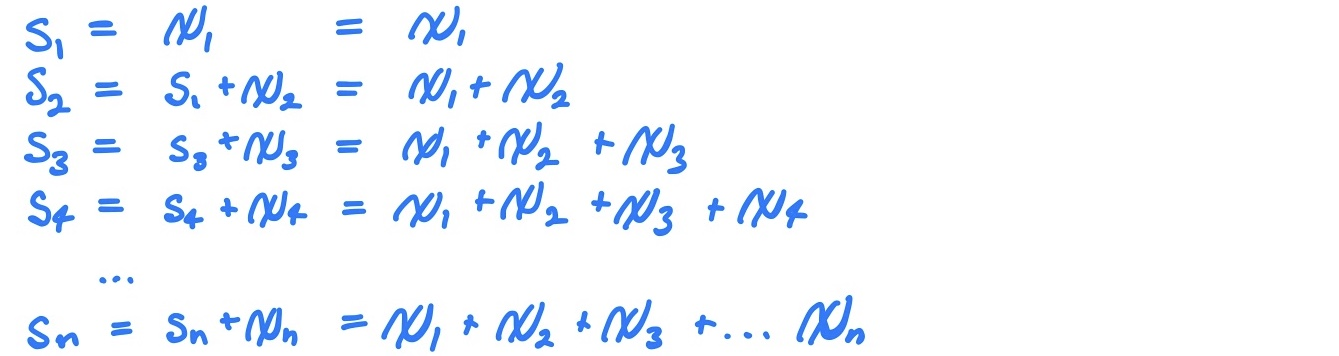
\includegraphics[width=5cm]{media/InfSeries/kdskfdsakj.jpeg}
\end{figure}

\hypertarget{header-n3150}{%
	%\newpage
\subsection{Common Series Types}\label{header-n3150}}

These are series that we are expected to memorise because they so often
appear in series problems (and moreover we we will need them for the
exam).

\hypertarget{header-n3152}{%
\subsubsection{Geometric Series (3.7.6 (a))}\label{header-n3152}}

The Geometric Series is Convergent if and only if \(\mid r \mid < \) :

\begin{figure}
\centering
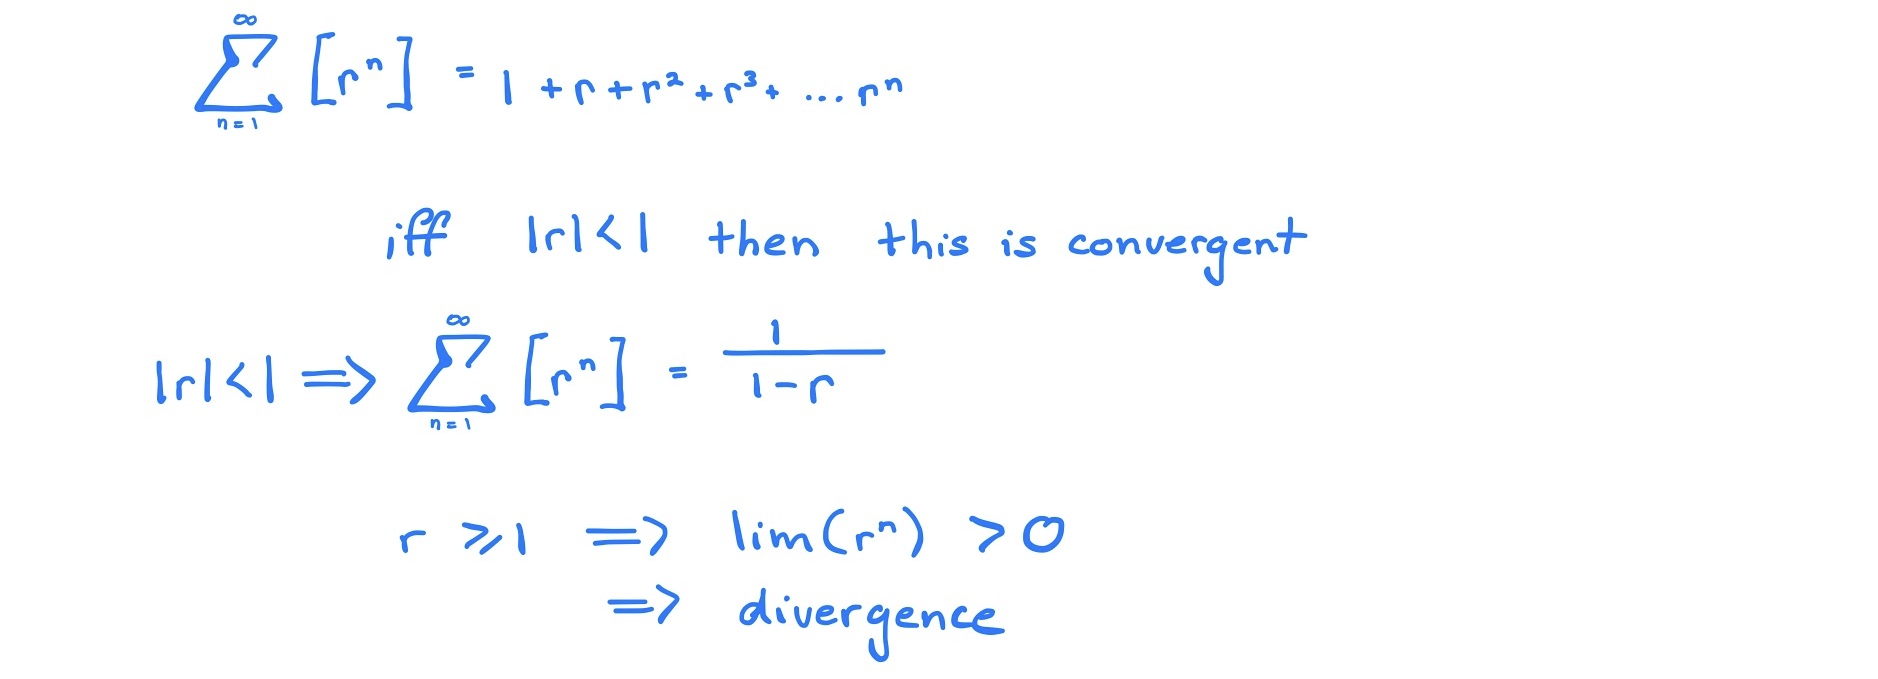
\includegraphics[width=5cm]{media/InfSeries/2B17FDDA-A24C-436F-B18E-73B69AF54A69.jpeg}
\caption{}
\end{figure}

\newpage
\hypertarget{header-n3155}{%
\subsubsection{Harmonic Series (3.7.6(b))}\label{header-n3155}}

\begin{figure}
\centering
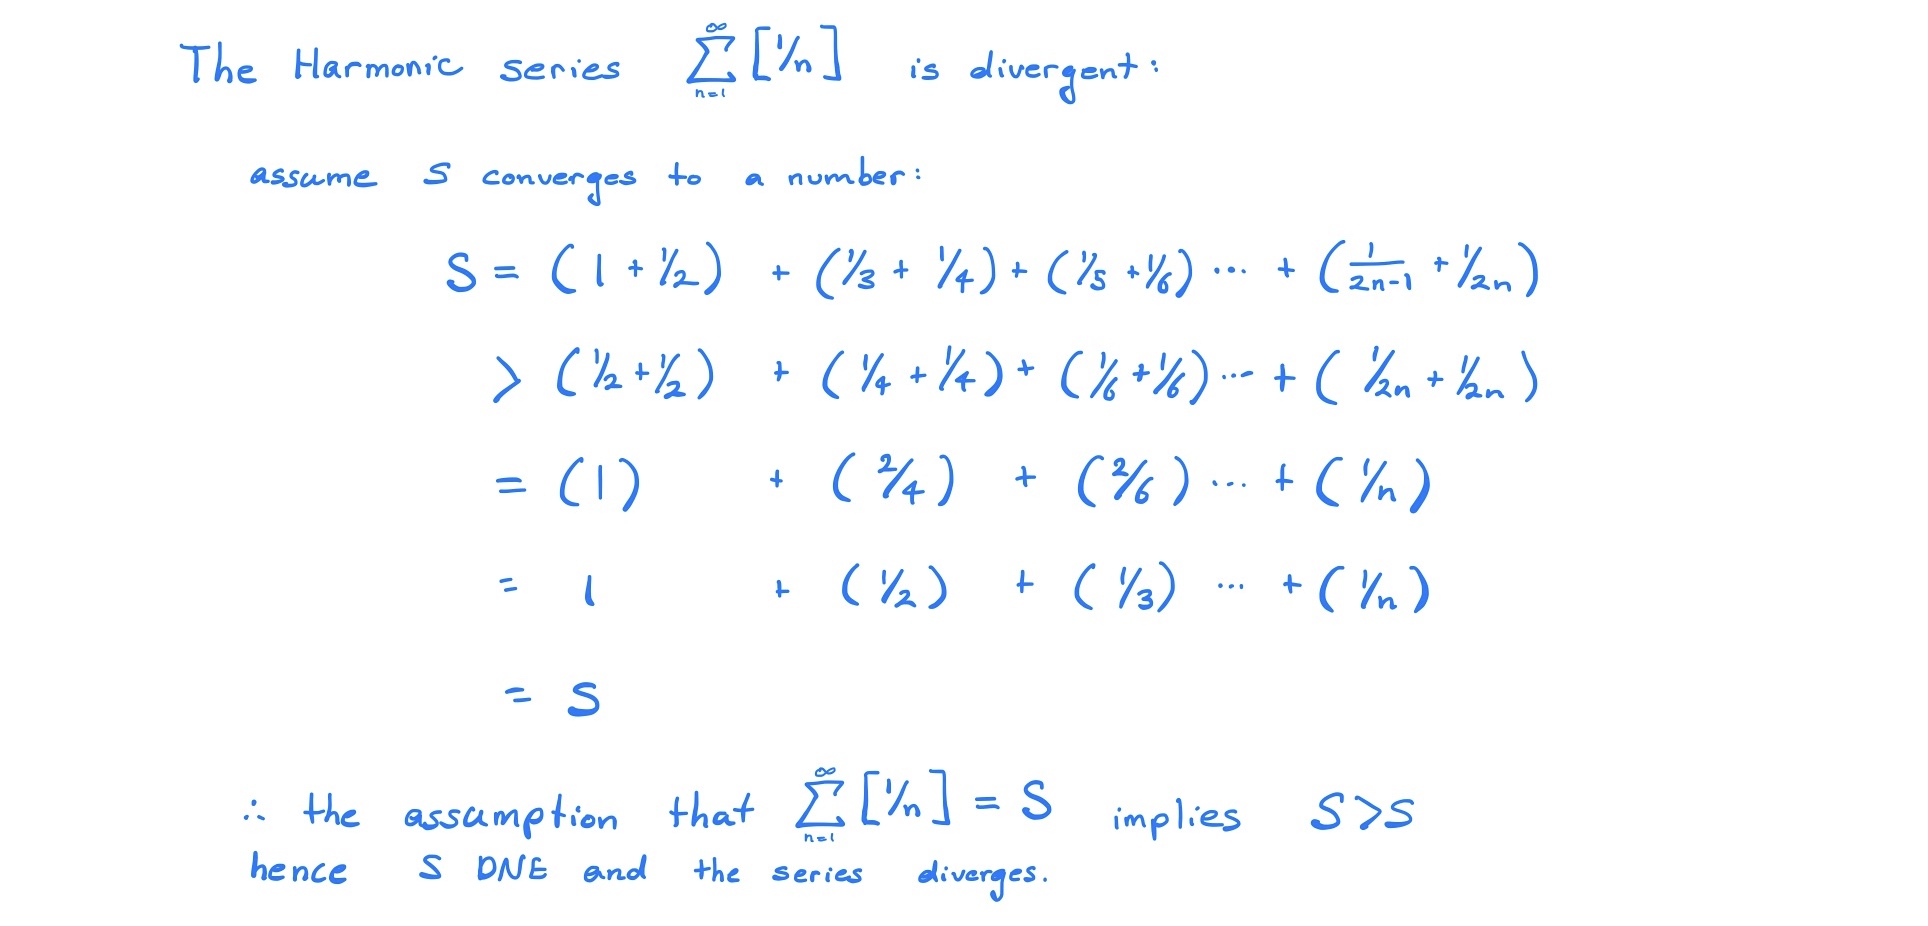
\includegraphics[width=5cm]{media/InfSeries/404880AA-8097-4857-B8DB-25933E988C53.jpeg}
\caption{}
\end{figure}

\hypertarget{header-n3157}{%
\subsubsection{\texorpdfstring{\(P\)-Series}{P-Series}}\label{header-n3157}}

\begin{figure}
\centering
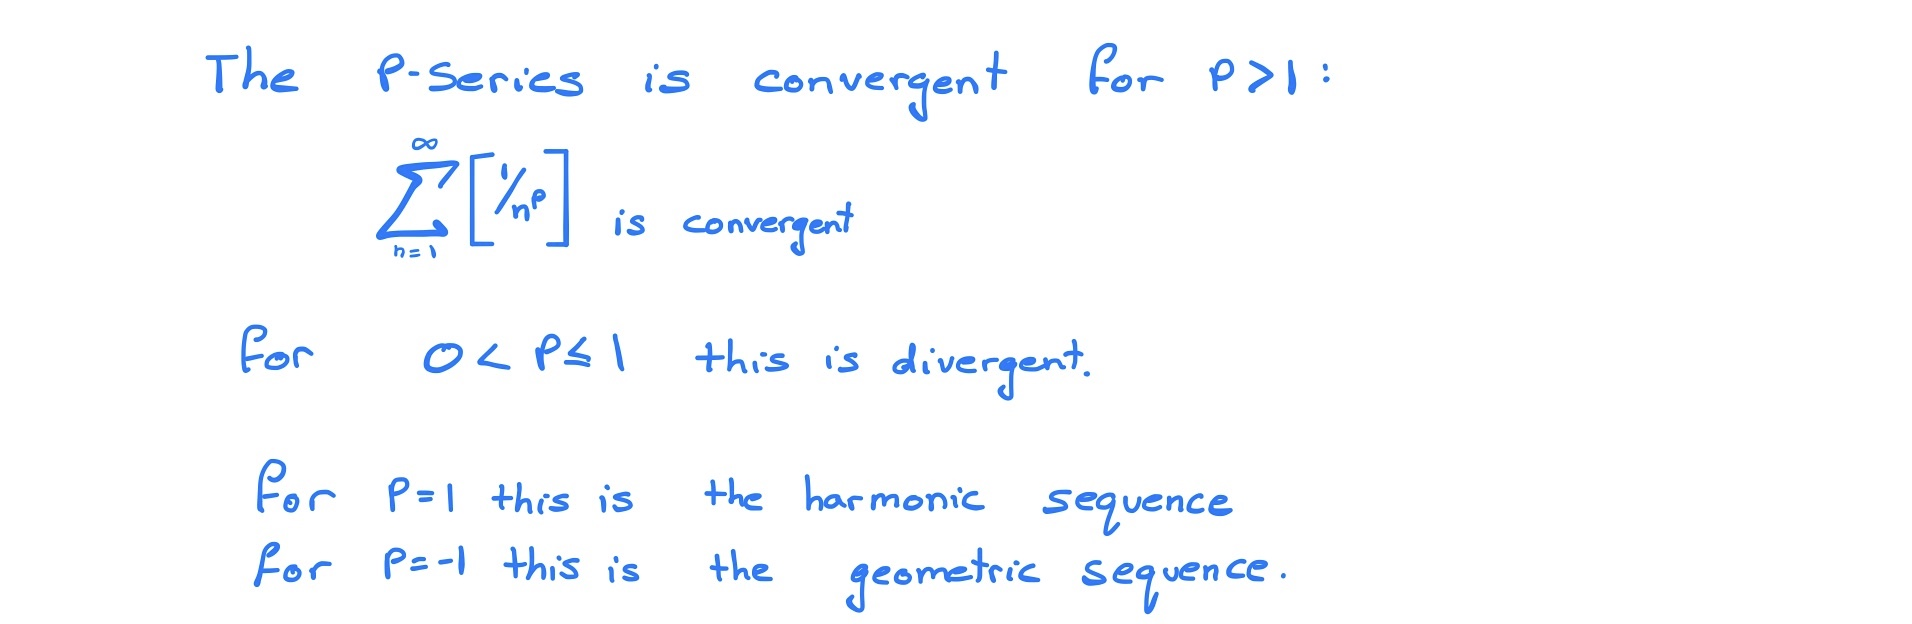
\includegraphics[width=5cm]{media/InfSeries/69F206AD-EF00-417C-95ED-31DAD675B9A5.jpeg}
\caption{}
\end{figure}

\newpage
\hypertarget{header-n3160}{%
\subsection{Properties of Series}\label{header-n3160}}

\hypertarget{header-n3161}{%
\subsubsection{\texorpdfstring{The \(n^\text{th}\) term
test}{The n\^{}\textbackslash text\{th\} term test}}\label{header-n3161}}

This is more or less a test for divergence, it is necessary that a
sequence \((x_n)\) has a limit of 0 in order for the series to be
convergent:

\[\exists L : \quad \sum_{n=1}^\infty \left[ x_n \right] = L \implies \lim(x_n)=0\]

be careful however because a sequence with a limit of 0 is not
sufficient to establish the convergence of a series:

\[\exists L : \quad \sum_{n=1}^\infty \left[ x_n \right] = L \nRightarrow \lim(x_n)=0\]

\hypertarget{header-n3167}{%
\subsubsection{Cauchy Criterion for series}\label{header-n3167}}

If a sequence is convergent it must be a Cauchy sequence, hence all
convergent series are composed of \emph{Cauchy Sequences} (as a
necessary but not sufficient condition).

So to be clear a series converges if and only if it is a \emph{Cauchy
Sequence}.

\hypertarget{header-n3170}{%
\subsubsection{Definitions}\label{header-n3170}}

\begin{itemize}
\item
  A Cauchy Sequence is:

  \begin{itemize}
  \item
    \(\forall \varepsilon > 0, \exists M : \enspace m,n \geq M \implies \mid s_m -s_n \mid = \left| x_{n+1} + x_{n+2} + x_{n+3} \dots x_m \right| < \varepsilon\)
  \end{itemize}
\item
  A Series Converges (which is an equivalent statement) if:

  \begin{itemize}
  \item
    \(\forall \varepsilon > 0, \exists M : \enspace ,n \geq N \implies \mid s_n -s \mid = \left| x_{1} + x_{2} + x_{3} \dots x_n \right| < \varepsilon\)
  \end{itemize}
\end{itemize}


\newpage
\hypertarget{header-n3182}{%
\subsection{Convergence Tests}\label{header-n3182}}

\hypertarget{header-n3183}{%
\subsubsection{Types of Convergence}\label{header-n3183}}

A series \(\sum [x_n]\) is \textbf{\emph{absolutely convergent}} if and
only if \(\sum \left[  \enspace \left| x_n \right| \enspace \right]\) ,
otherwise the series is said to be conditionally convergent.

This is important because
\(\textsf{the convergence of } \sum \left[  \enspace \left| x_n \right| \enspace \right] \implies \textsf{the convergence of} \sum [x_n]\)

Below the tests have been split into three categories:

\begin{itemize}
\item
  Comparison Tests

  \begin{itemize}
  \item
    These establish non-absolute convergence but are broadly applicable
    and so are introduced early
  \end{itemize}
\item
  Absolute Convergence Tests

  \begin{itemize}
  \item
    These establish absolute convergence.
  \end{itemize}
\item
  Non-Absolute Convergence Tests

  \begin{itemize}
  \item
    These are useful for \emph{alternating Series} and series that
    change sign as they progress (e.g. \(\frac{sin(n)}{n}\))
  \end{itemize}
\end{itemize}

\hypertarget{header-n3203}{%
\subsubsection{Choosing a Test}\label{header-n3203}}

Choosing the right test can be difficult, hence I have included an
appendix with a
\href{http://tutorial.math.lamar.edu/Classes/CalcII/SeriesStrategy.aspx}{flow
chart} \footnote{Strategy for Series,
  http://tutorial.math.lamar.edu/Classes/CalcII/SeriesStrategy.aspx}
that we should probably memorise for want of the exam



\hypertarget{header-n3206}{%
\subsubsection{Manipulating Series}\label{header-n3206}}

Sometimes you'll be given a series in an odd way for example:

\[S_n = \sum^\infty_{n=1} \left[ \frac{1}{(3n-2)\cdot (3n+1)} \right]\]

Now this could be shown to be convergent using the limit comparison test
(which is below) but if you are asked to find the value to which the
series converges to there is a bit more work involved.

Generally if you are asked to find what value a series converges to it
will be either:

\begin{itemize}
\item
  A Geometric Series (3.7.6(a) of TB), or
\item
  A telescoping Series
\end{itemize}

Geometric Series have already been shown, but a telescoping series is
new and not covered in the textbook, basically, it is a series where
most of the terms cancel out by way of rearrangement and grouping to
leave only one or two terms left.



\hypertarget{header-n3218}{%
\paragraph{Partial Fractions}\label{header-n3218}}

Often it is necessary to manipulate the terms somewhat in order for them
to exhibit the cancelling/telescoping property, often by way of partial
fractions (remember from \emph{Mathematics1B}), for an example of this
refer to Q3(c) of the corresponding tutorial
\(\tiny \textsf{(tutorial \#4 of wk 4 material, due wk. 5, topic 3 from learning guide)}\)

In this case because the provided series is not a geometric series it
must be a telescoping series (because otherwise we wouldn't be asked to
find the value to which it converges to, we only know how to find the
convergence values of those two series, so we know it's telescoping, in
order to get it into a form that will work, use partial fractions
\footnote{Partial Fractions,
  \href{Pauls\%20Calculus}{http://tutorial.math.lamar.edu/Classes/CalcII/PartialFractions.aspx}}

\begin{figure}
\centering
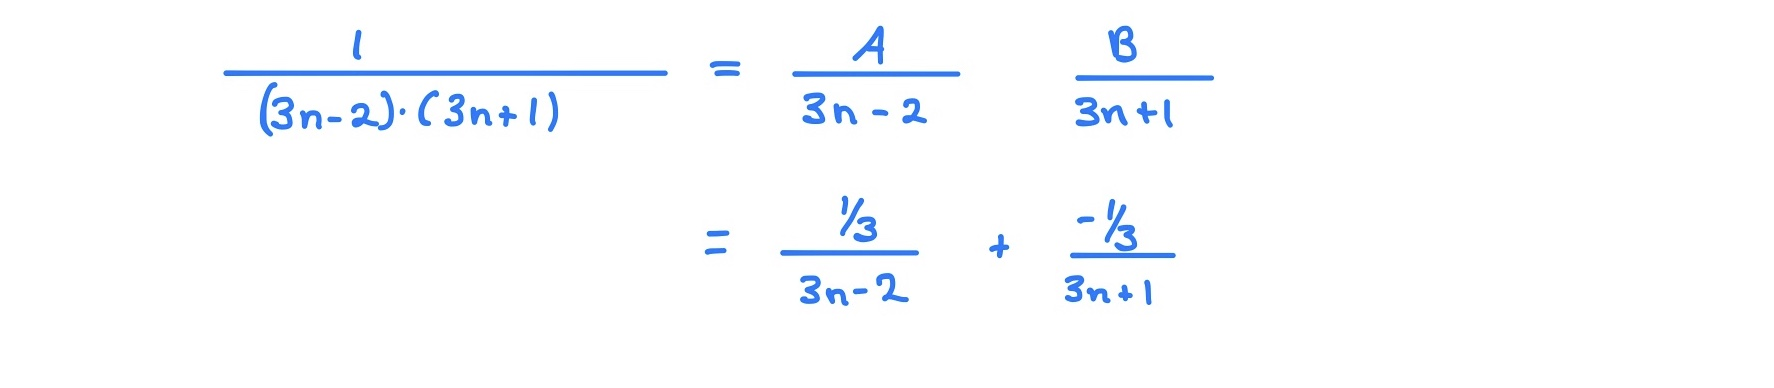
\includegraphics[width=5cm]{media/InfSeries/55CCA5D8-0B0A-438D-A991-6DB931F19D72.jpeg}
\caption{}
\end{figure}

From here we would manipulate the series using grouping and
rearrangement

\hypertarget{header-n3223}{%
\paragraph{Grouping Series}\label{header-n3223}}

Grouping terms in a series does not affect the value to which it
converges,

\begin{itemize}
\item
  This flows from the associativity of addition, a property exhibited by
  the \(\mathbb{R}\) which is the codomain of the sequence function
\end{itemize}

So in the above example the regrouping necessary to demonstrate the
telescoping nature:

\begin{figure}
\centering
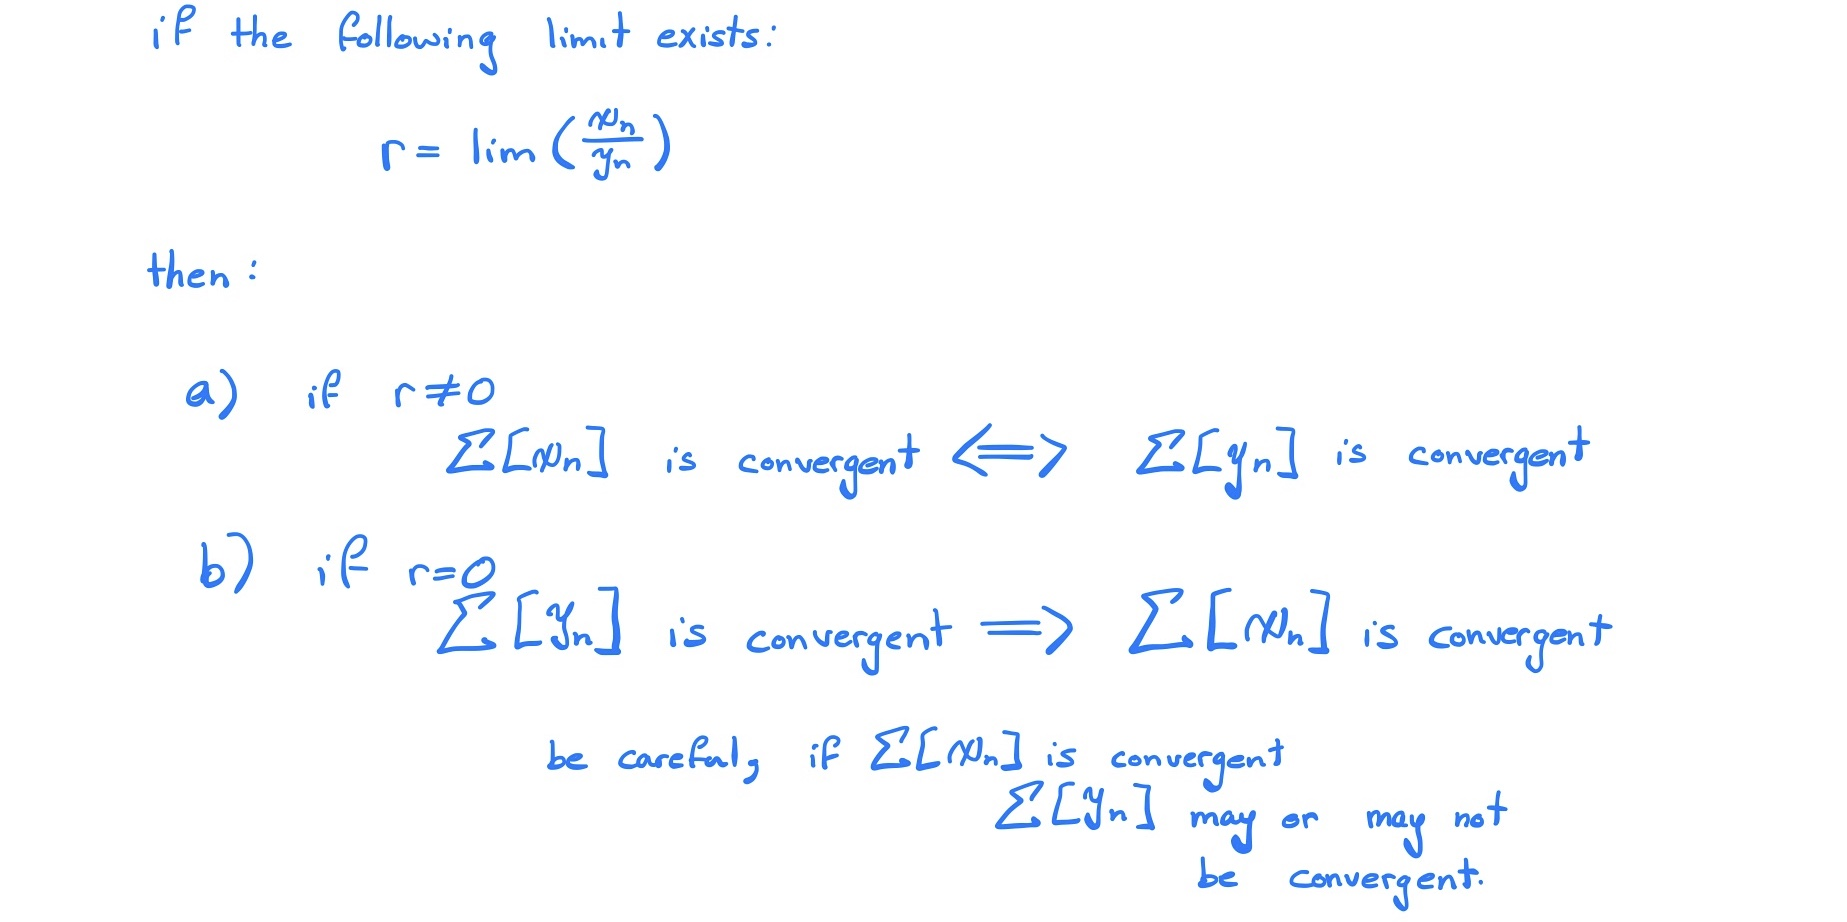
\includegraphics[width=5cm]{media/InfSeries/67331FF8-C7AD-4BE3-ADAE-2D291C4A5D89.jpeg}
\caption{}
\end{figure}

\newpage
\hypertarget{header-n3232}{%
\paragraph{Rearrangements (9.1.5)}\label{header-n3232}}

If a series is absolutely convergent then you can rearrange the terms
and the series will converge to the same value (otherwise you can't so
be careful)

\begin{itemize}
\item
  So say you have some series and you rearrange it, if this new series
  is absolutely convergent thet it's fine.
\item
  However, if you rearrange some series and the new series is only
  conditionally convergent, then the rearrangement wasn't logically
  valid and this convergence value is erroneous. 
\end{itemize}

So in our example the series is absolutely convergent so we could
rearrange it:

\begin{figure}
\centering
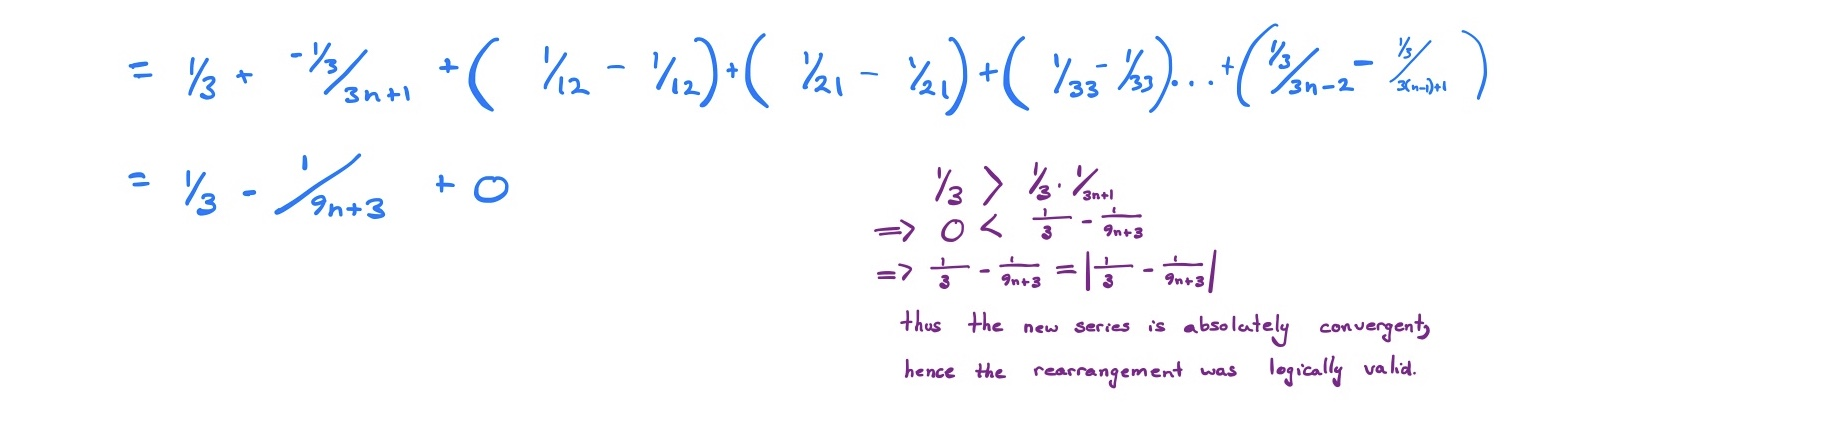
\includegraphics[width=5cm]{media/InfSeries/83FE5712-DC18-44D6-A9A3-FF7CB63F6AE9.jpeg}
\caption{}
\end{figure}

\newpage
\hypertarget{header-n3241}{%
\subsubsection{Identities to remember}\label{header-n3241}}

For the exam We need to remember these identities:

\hypertarget{header-n3243}{%
\paragraph{\texorpdfstring{Limit of
\(e^\frac{1}{n}\)}{Limit of e\^{}\textbackslash frac\{1\}\{n\}}}\label{header-n3243}}

\begin{figure}
\centering
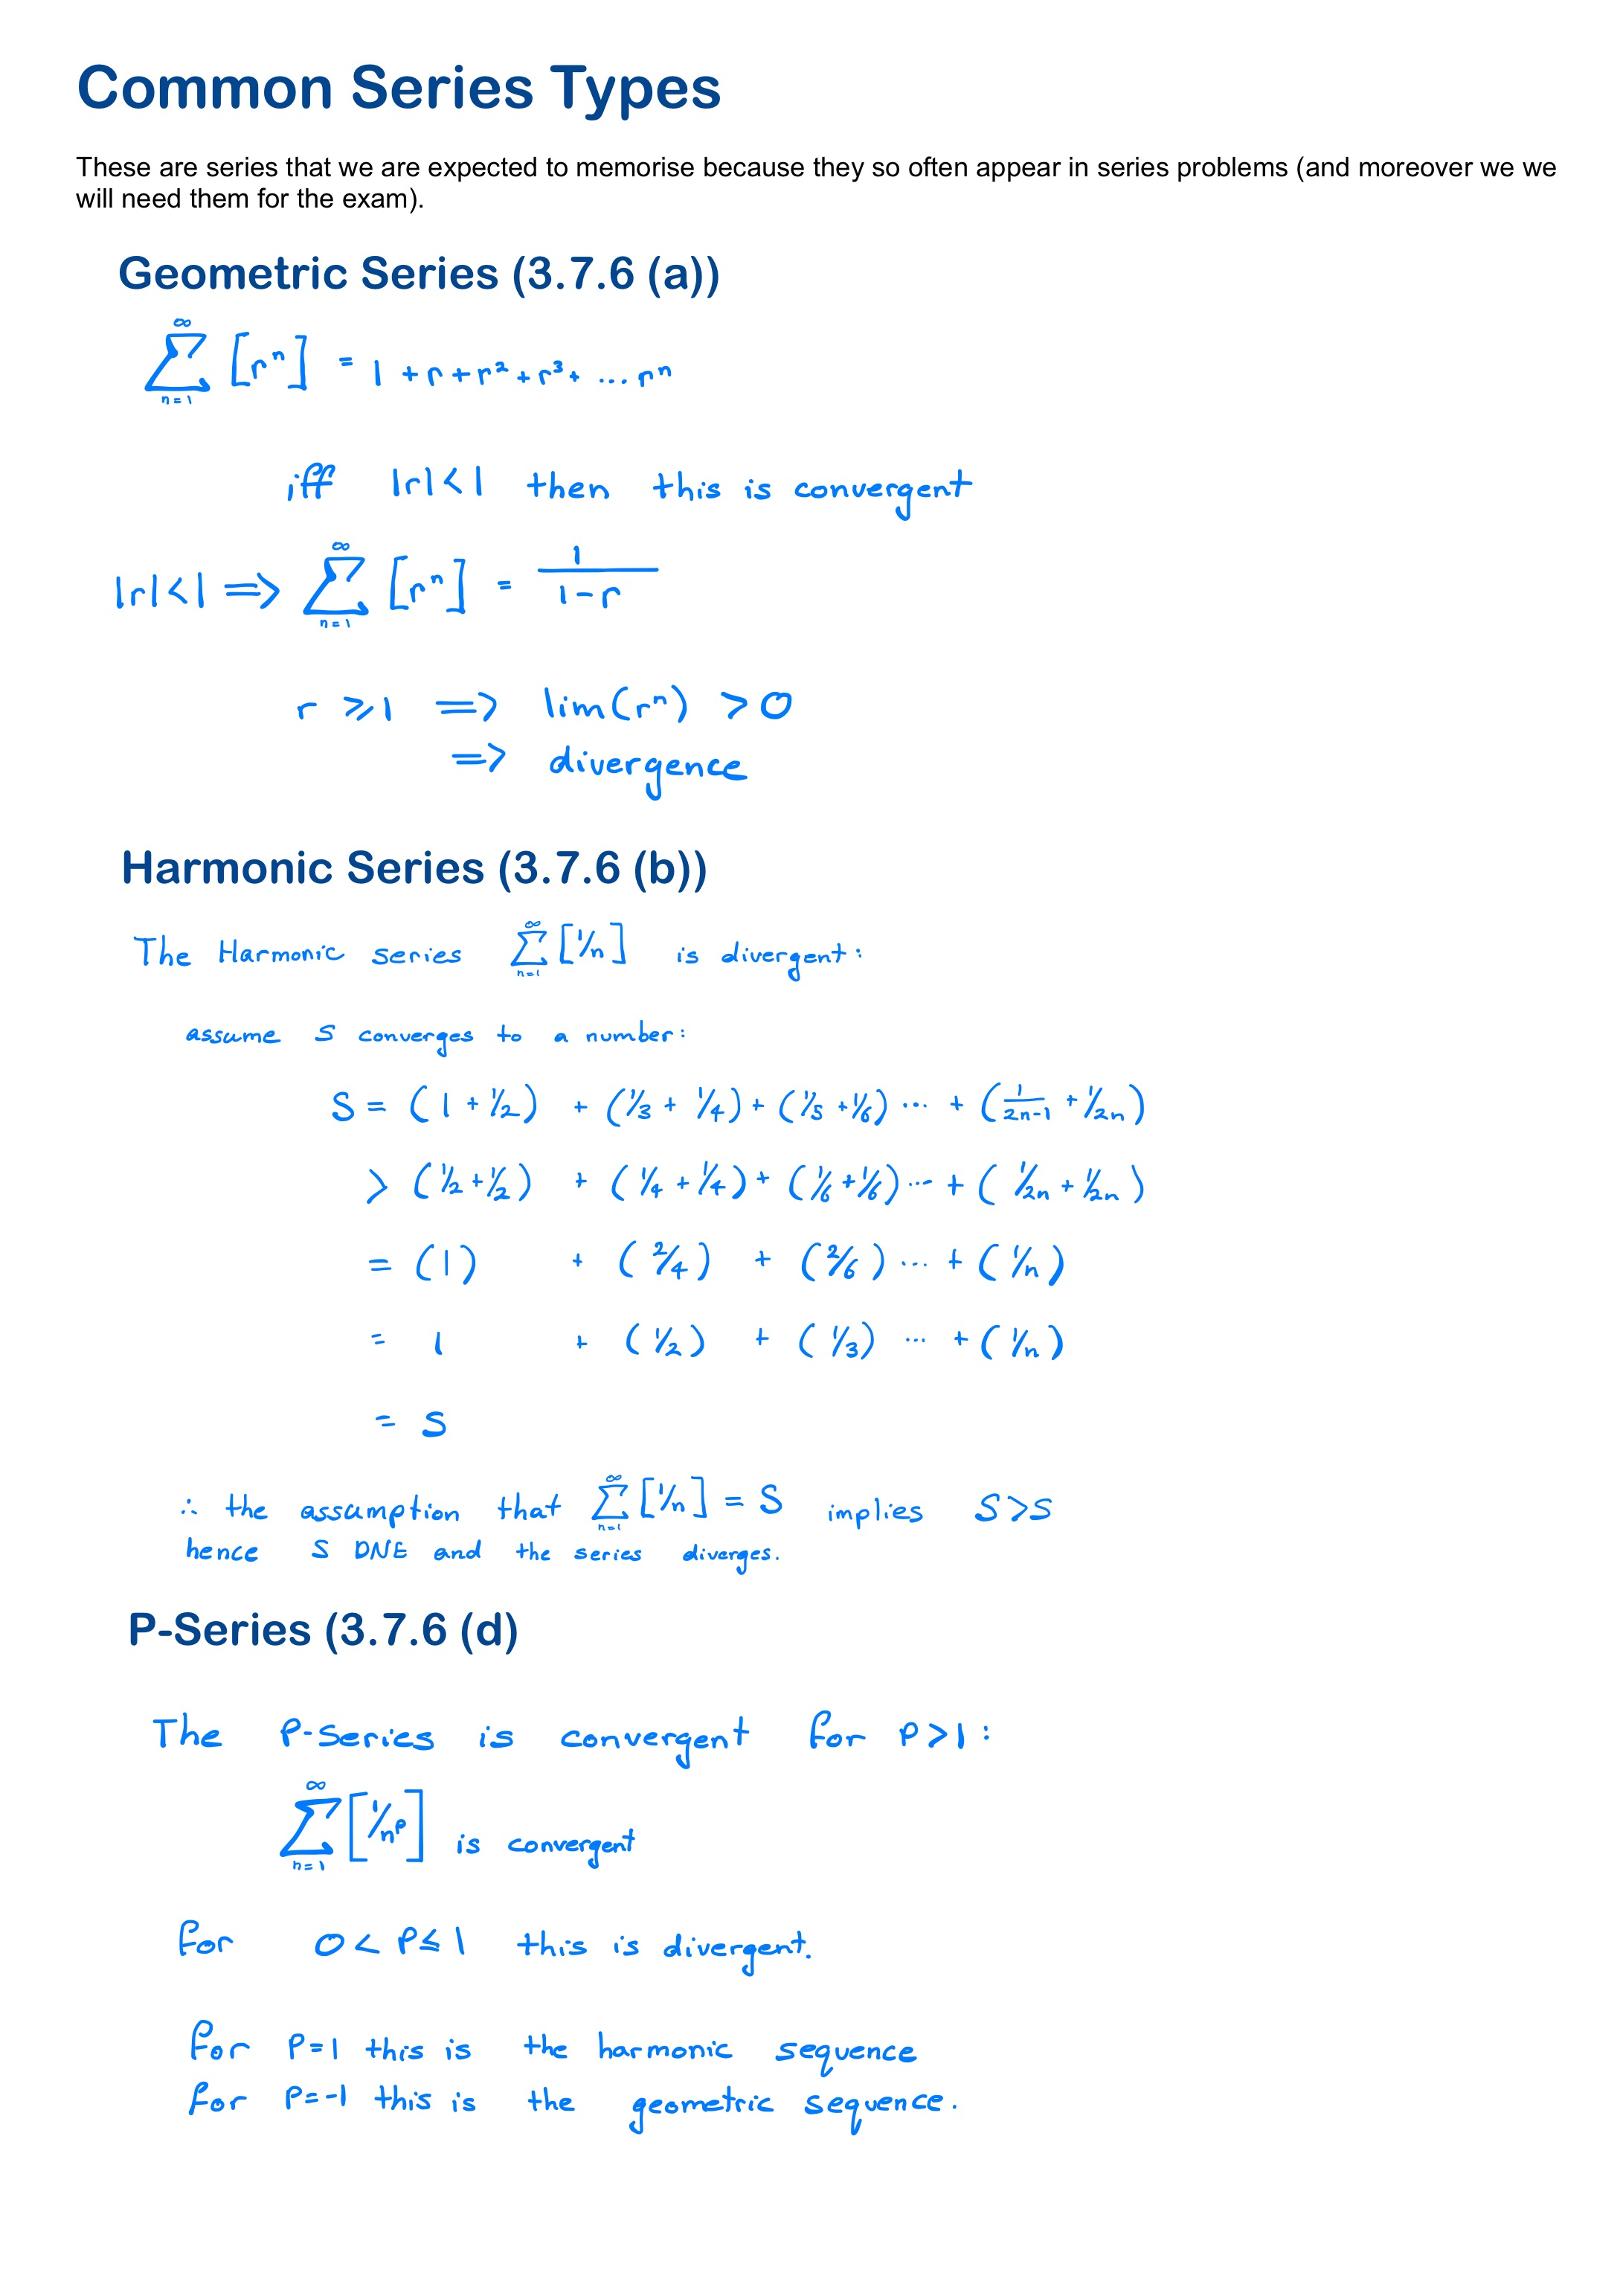
\includegraphics[width=5cm]{media/InfSeries/5E521A99-BC9F-40B8-8FE7-4B35EB40DC43.jpeg}
\caption{}
\end{figure}

\hypertarget{header-n3245}{%
\paragraph{Dealing with Inequalities}\label{header-n3245}}

\begin{figure}
\centering
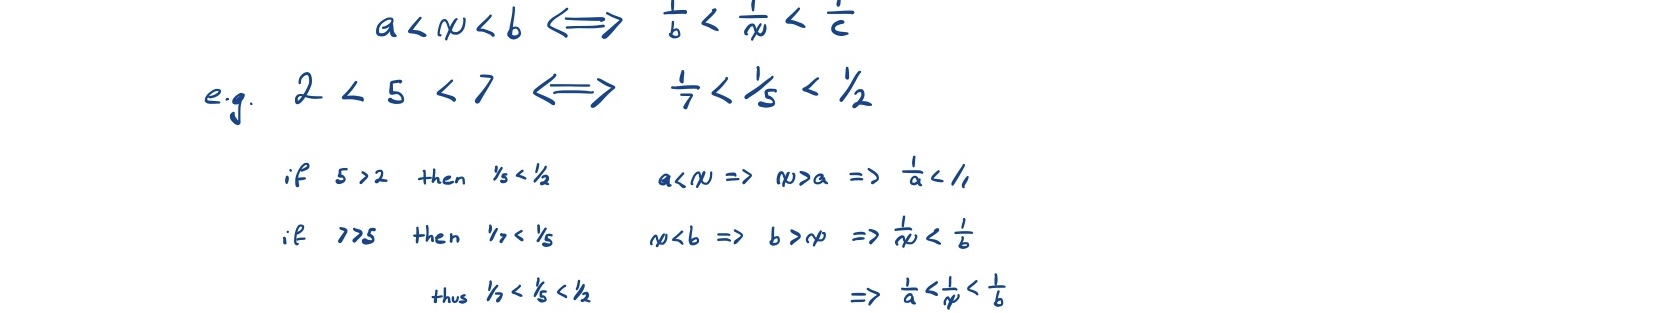
\includegraphics[width=5cm]{media/InfSeries/C613EA1A-E507-4DED-8B75-9A7B87BA17C1.jpeg}
\caption{}
\end{figure}

\newpage

\hypertarget{header-n3247}{%
\subsubsection{Comparison Tests}\label{header-n3247}}

\hypertarget{header-n3248}{%
\paragraph{Comparison Test (3.7.7)}\label{header-n3248}}

\begin{figure}
\centering
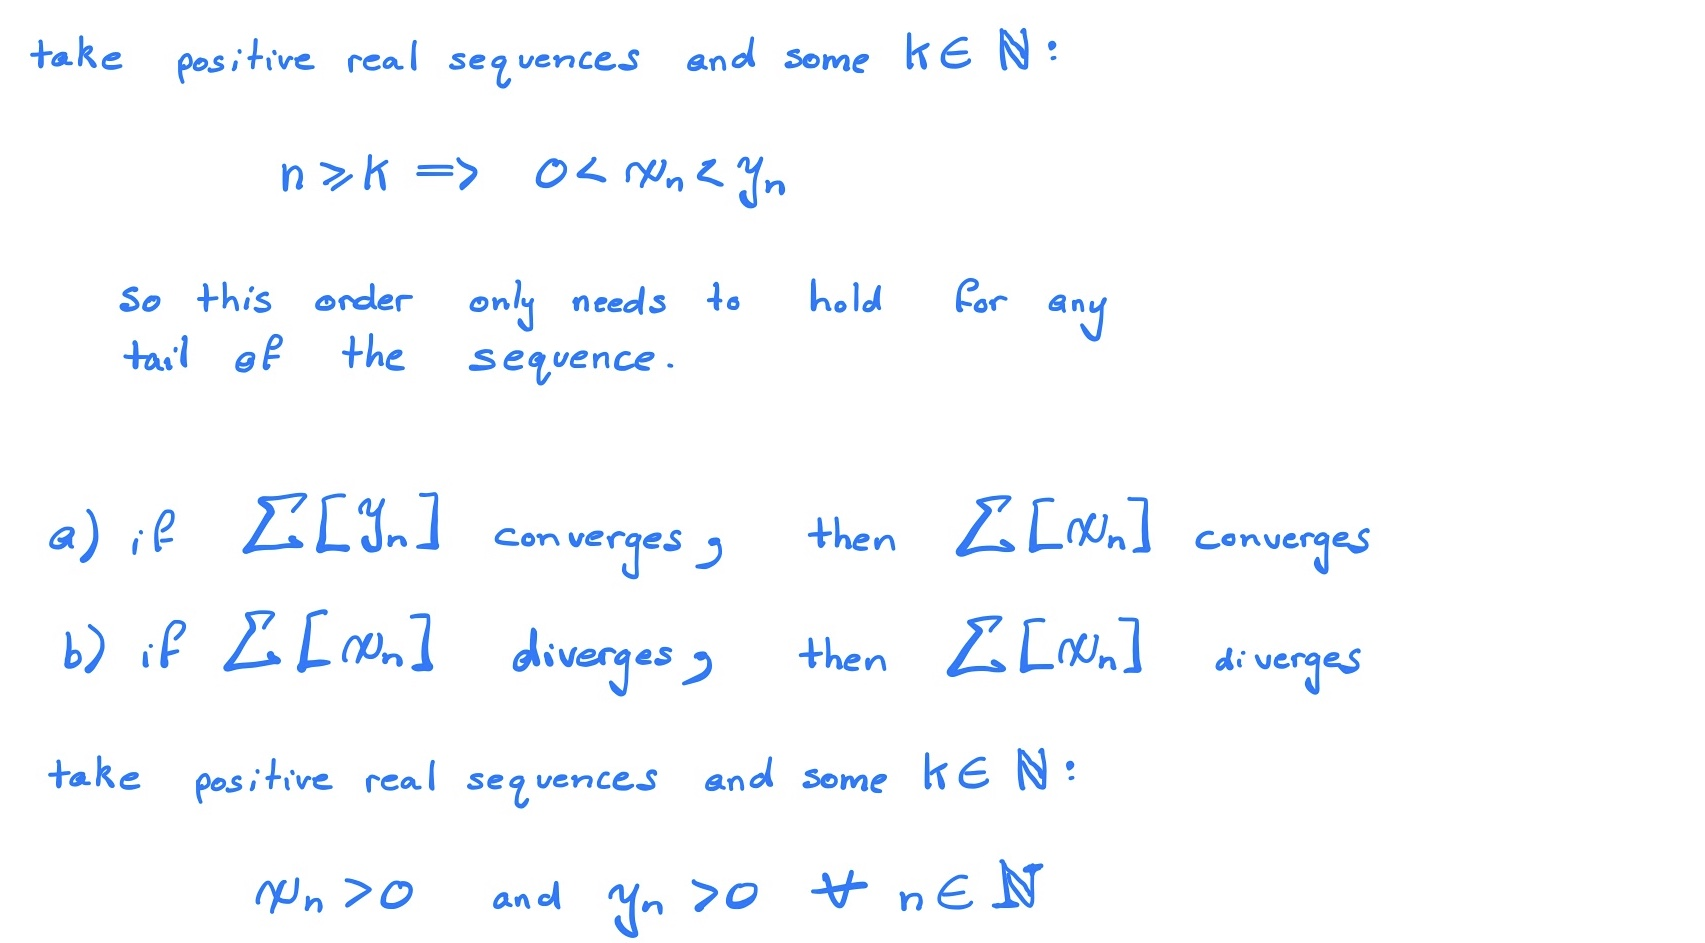
\includegraphics[width=5cm]{media/InfSeries/FD08303A-128F-49B5-80ED-4EBD48B1A48F.jpeg}
\caption{}
\end{figure}

\hypertarget{header-n3250}{%
\paragraph{Limit Comparison Test (3.7.8)}\label{header-n3250}}

Sometimes it can be difficult to establish the inequealities of the
first test and a ratio would be easier to use, in that case this test
can be used:
\ \\
\ \\
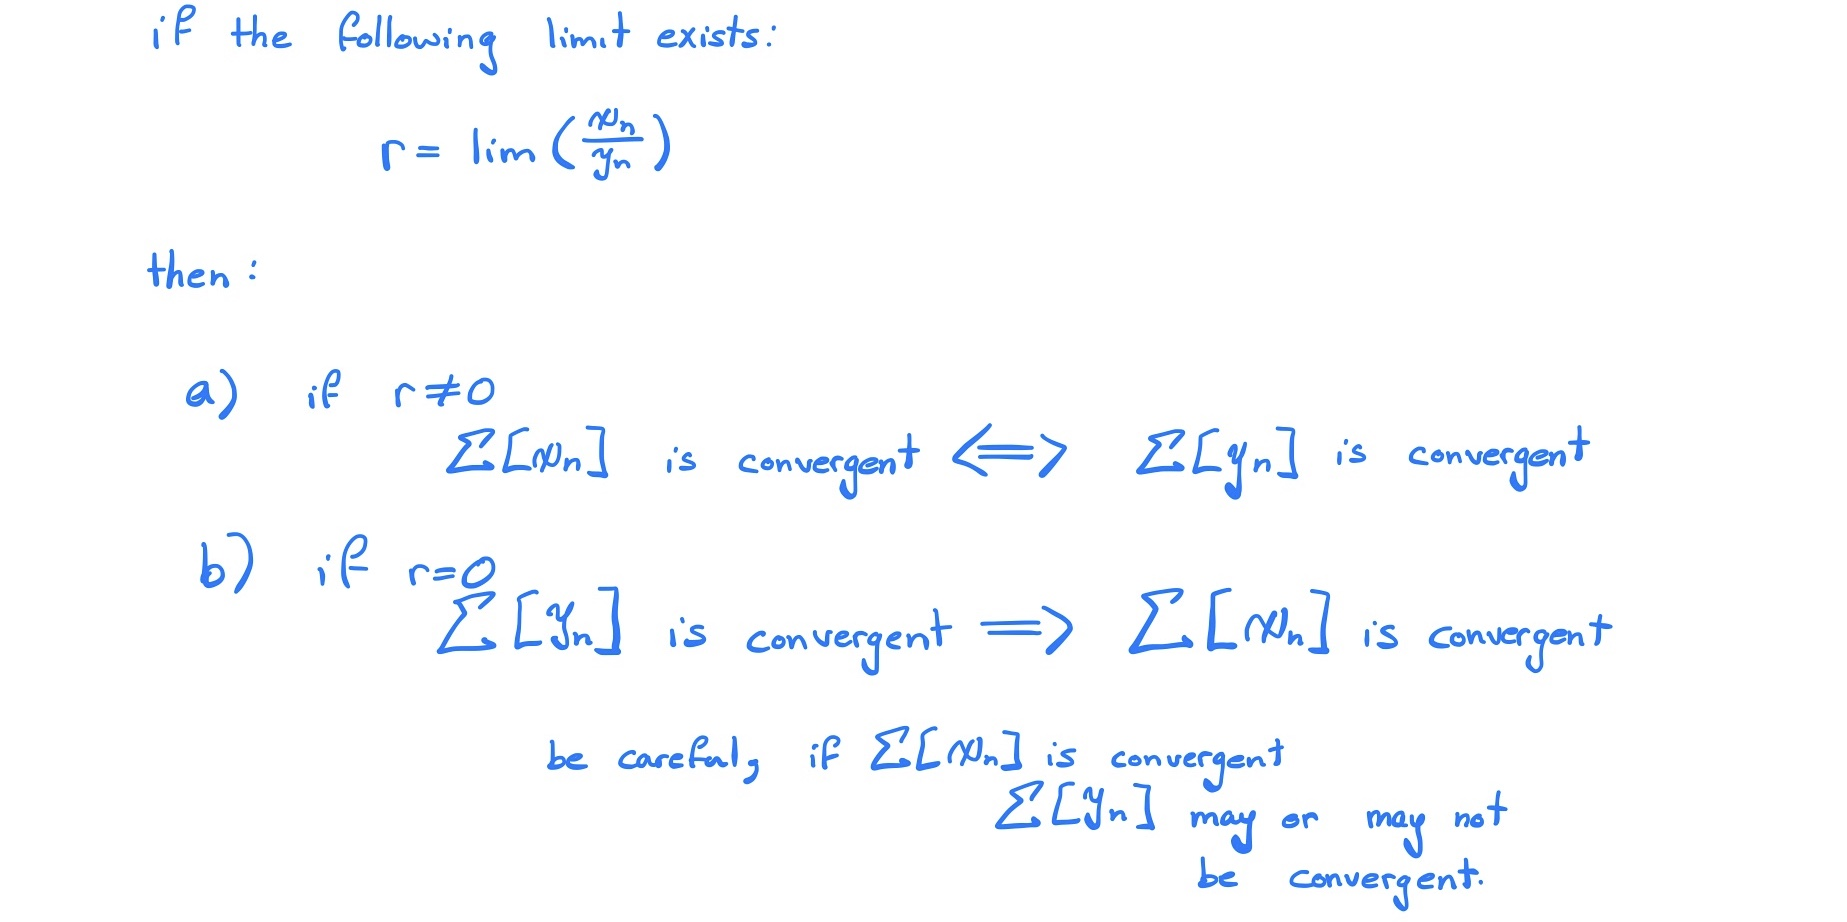
\includegraphics[width=5cm]{media/InfSeries/67331FF8-C7AD-4BE3-ADAE-2D291C4A5D89.jpeg}

\hypertarget{header-n3253}{%
\subsubsection{Absolute Convergence Tests}\label{header-n3253}}

If these tests are satisfied they will establish that the series is
absolutely convergent.

\hypertarget{header-n3255}{%
\paragraph{Limit Comparison Test II (9.2.1) (For Absolute
Convergence)}\label{header-n3255}}

This version of the test is useful for establishing absolute
convergence, it may be more difficult to establish however.

\begin{figure}
\centering
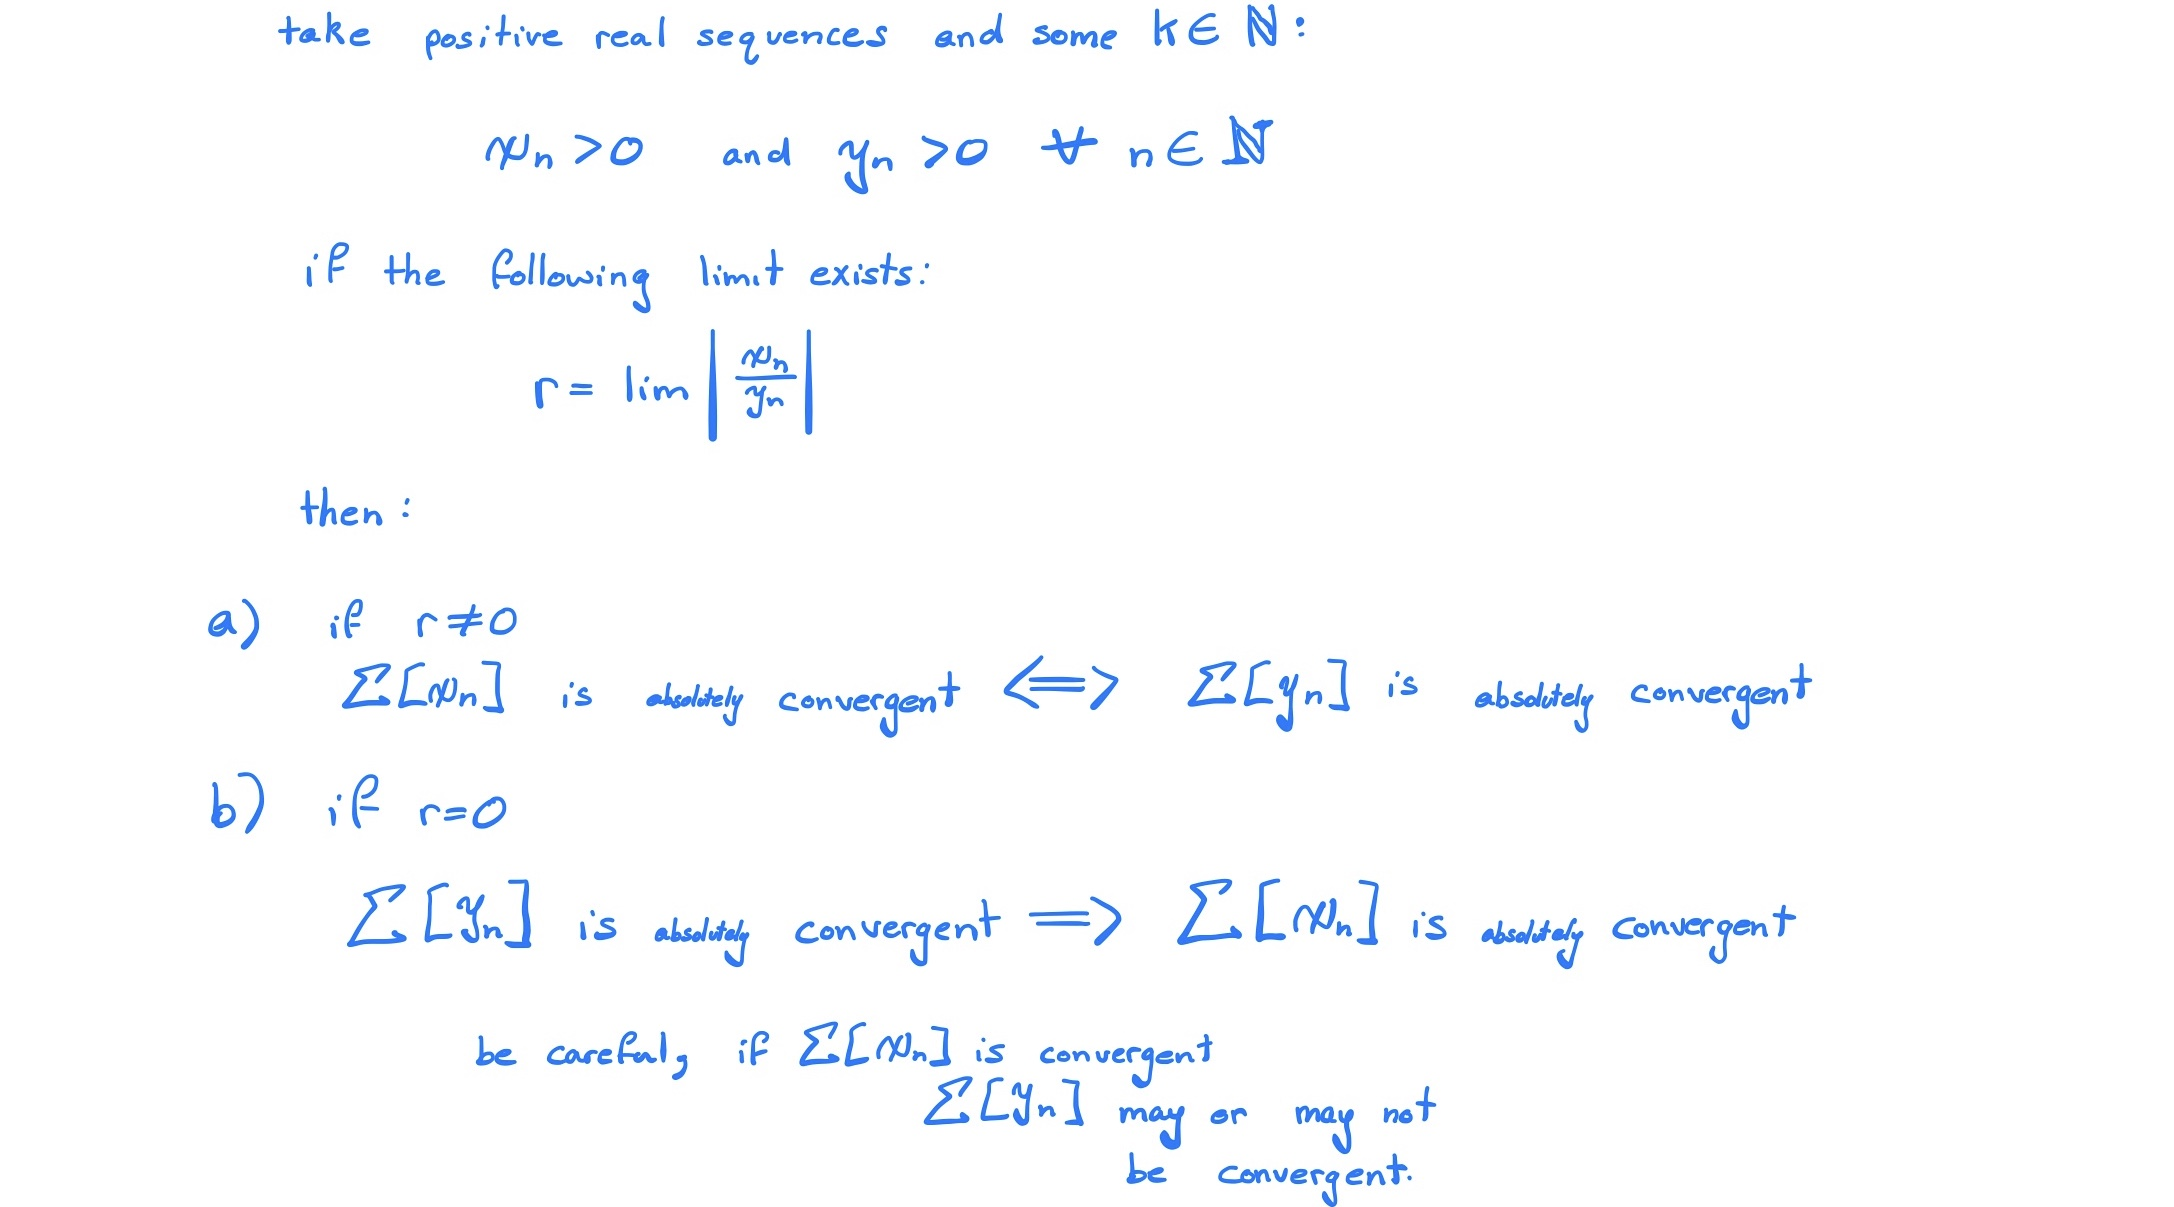
\includegraphics[width=5cm]{media/InfSeries/DEEDB59D-00EA-4BF3-A5F9-7571412B11C2.jpeg}
\caption{}
\end{figure}

\newpage
\hypertarget{header-n3259}{%
\paragraph{Ratio Test (9.2.4)}\label{header-n3259}}

\hypertarget{header-n3261}{%
\subparagraph{Generalised D'Alambert}\label{header-n3261}}

This can be useful where the ratio test fails for want of \((-1)^{n+1}\)
because the \(\limsup()\) operator will strip that way for a \((+1)\).

It is worth remembering that a sequence \((x_n)\) is convergent if and
only if:

\[\liminf(x_n) = \limsup(x_n)=\lim(x_n)\]

In this test however, we simply need to show that the \(\limsup\) exists
(which it will if the ratio-sequence has an upper bound), it isn't
necessary to show that the ratio-sequence is convergent.

\begin{itemize}
\item
  (However, it is necessary that the sequence which generates the series
  converges to 0, otherwise the series will be divergent)
\end{itemize}

\newpage 

\hypertarget{header-n3270}{%
\paragraph{Root Test}\label{header-n3270}}

\begin{figure}
\centering
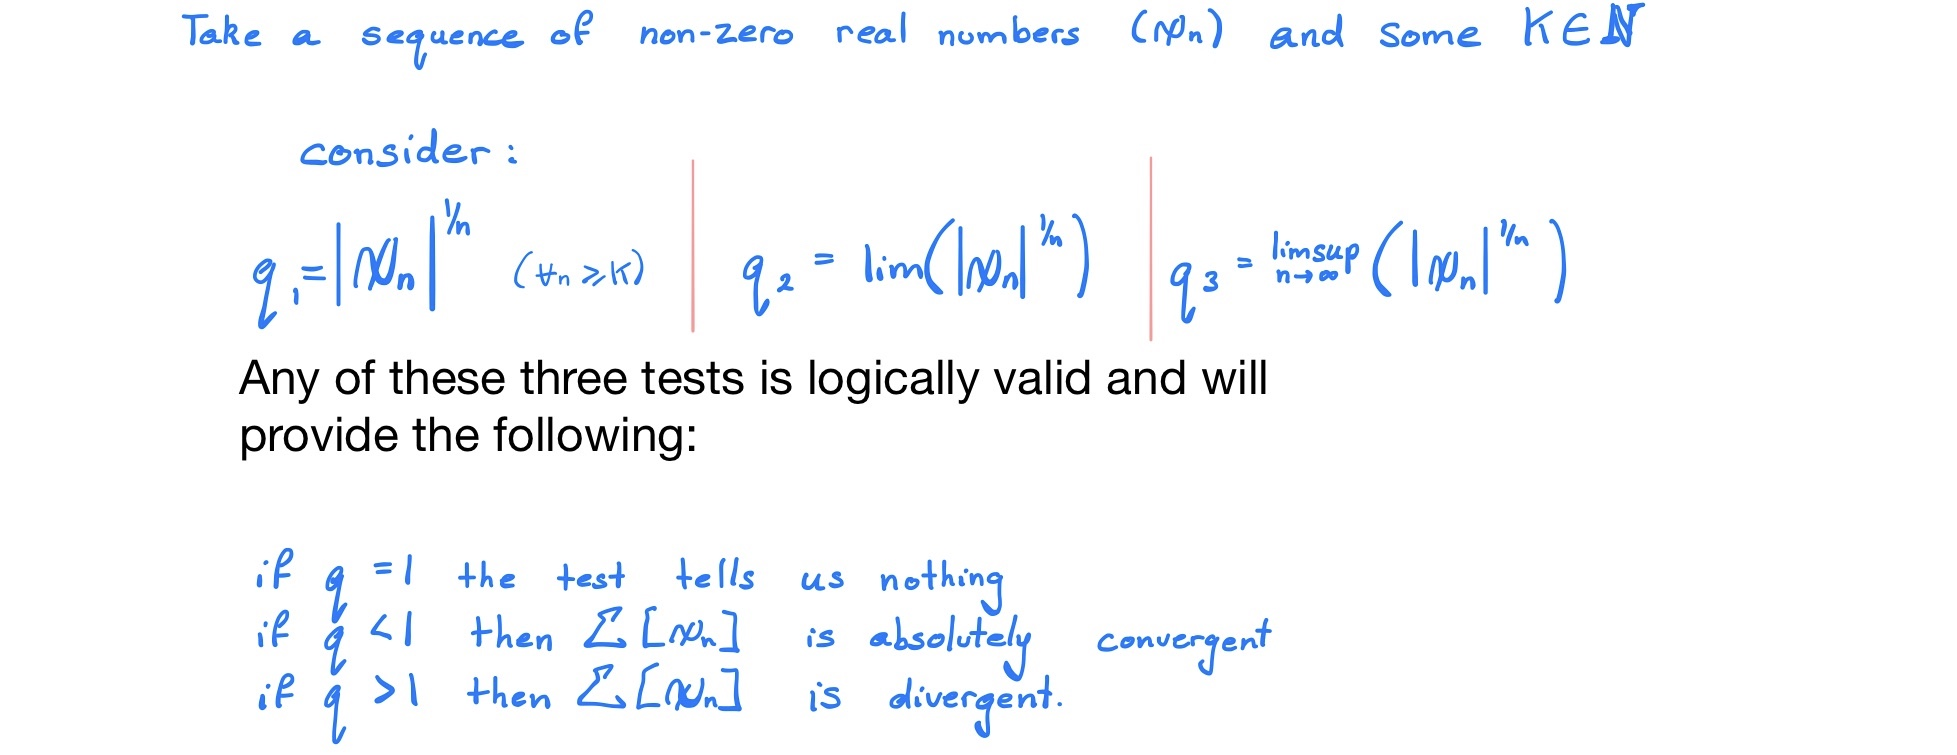
\includegraphics[width=5cm]{media/InfSeries/8D469008-5118-4138-808A-3A9480B23FA5.jpeg}
\caption{}
\end{figure}

\hypertarget{header-n3274}{%
\subparagraph{\texorpdfstring{Generalised \emph{Cauchy}
Test}{Generalised Cauchy Test}}\label{header-n3274}}

This can be useful where the root test fails for want of \((-1)^n\), the
\(\limsup()\) operator will strip that away for a \((+1)\).

\hypertarget{header-n3276}{%
\paragraph{Integral Test}\label{header-n3276}}

If the series is of a function that is positive and ecreasint, then the
series could converge if and only if the integral converges:

Let \(f(k)\) be a positive decreasing function and let \(k\) be some
natural number:

\[\exists L\in \mathbb{R} : \enspace L = \sum^\infty_{n=k} \left[ f(k) \right] \ \iff \int_\infty^k \! f(x) \, \mathrm{d}x = \lim_{b\rightarrow\infty}\left( \int_b^k \! f(x) \, \mathrm{d}x\right)\]

Or basically the series will converge if and only if the corresponding
integral converges,

\begin{itemize}
\item
  This flows from the notion that the area under a continuous curve is
  going to be greater than the various term values, hence by the
  comparison test it's going to converge.
\item
  this is a test for absolute convergence because the terms of the
  sequence that generates the series are strictly positive as a
  prerequisite anyway.
\end{itemize}

\newpage 

\hypertarget{header-n3286}{%
\subsubsection{Non-Absolute Convergence Tests}\label{header-n3286}}

\hypertarget{header-n3287}{%
\paragraph{Definition of an Alternating Sequence
(9.3.1)}\label{header-n3287}}

An alternating sequence is a sequence that changes sign at each
iteration, so for example \((x_n) = \frac{(-1)^{n+1}}{n}\) is an
alternating sequence because at each succession the sequence changes
sign \((x_n) = \frac{\sin(n}{n}\) is not an alternating sequence because
the terms doesn't alternate at each succession:

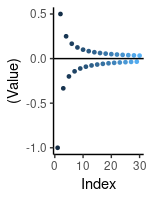
\includegraphics[width=5cm]{media/InfSeries/Rplot.png}
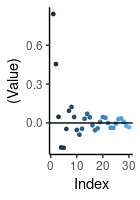
\includegraphics[width=5cm]{media/InfSeries/Rplot01.png}

\hypertarget{header-n3292}{%
\paragraph{Alternating Series Test}\label{header-n3292}}

Take a decreasing sequence of positive numbers \((Z_n)\), :

\begin{itemize}
\item
  If the sequence is such that:

  \begin{itemize}
  \item
    \(Z_{n+1} < Z_n \enspace  \enspace \wedge \enspace Z_n > 0 \qquad \forall n \in \mathbb{n}\)
  \end{itemize}
\item
  Then the series will be convergent:

  \begin{itemize}
  \item
    \(\exists L \in \mathbb(R): \enspace \sum^\infty_{n=1} \left[ (-1)^{n+1} \cdot Z_n \right]\)
  \end{itemize}
\end{itemize}

So basically if the sequence is decreasing, then the series of the
alternating sequence will hence converge.

\hypertarget{header-n3307}{%
	\newpage
\paragraph{Partial Summation Formula (Abel's
Lemma)}\label{header-n3307}}

Let \(X: = \left( x_n \right)\) and \(Y:= \left( y_n \right)\) by
sequences in \(\mathbb{R}\) and let the partial sums of
\(\sum\left( y_n \right)\) be denoted by \(\left( s_)n \right)\) with
\(s_0 : = 0\)

\[\sum_{k=n+1}^{m}\left[ x_ky_k \right]=\left( x_ms_m - x_{n+1}s_n \right) + \sum{k=n+1}^{m-1}\left( x_k-x_k+1 \right)s_k
  \label{partsum}\]



\hypertarget{header-n3311}{%
\paragraph{Dirichlet's Test}\label{header-n3311}}

\begin{figure}
\centering
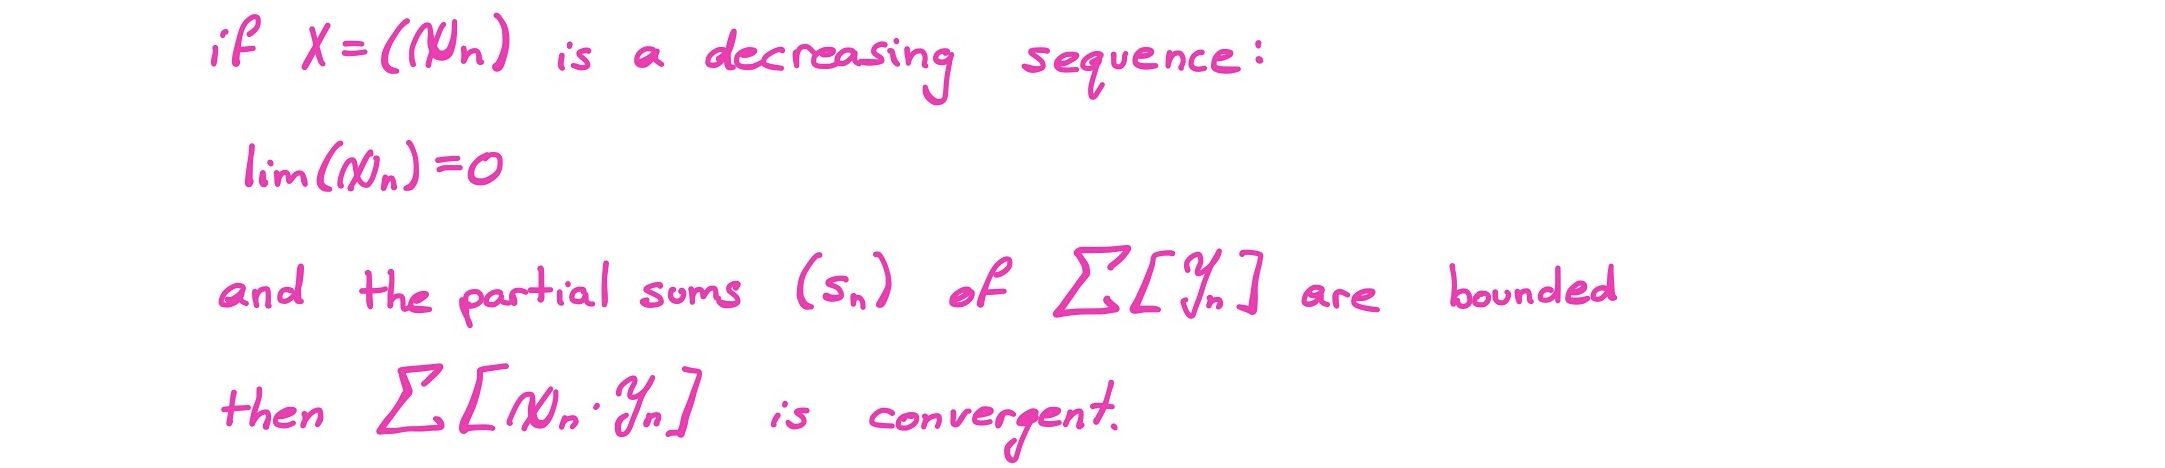
\includegraphics[width=5cm]{media/InfSeries/BE23258A-CC18-49A6-AABB-E71063CAF34C.jpeg}
\caption{}
\end{figure}

\hypertarget{header-n3314}{%
\paragraph{Abel's Test}\label{header-n3314}}

\begin{figure}
\centering

\includegraphics[width=5cm]{media/InfSeries/6360D524-9307-4308-94C1-BCA6D2E0ECE7.jpeg}
\caption{}
\end{figure}

\end{document}
 %exemplar not tutorial problem
\documentclass[class=article, crop=false]{standalone}
\usepackage{./resources/style}
\title{Cauchy Criterion Problem (Textbook; Problem 2, (a))}
\begin{document}
\section{3.5 - Cauchy Criterion Problems (Textbook); Problem 2, (a)}
\subsection{Problem}
Show that the follwoing sequence is a Cauchy Sequence

\begin{align}
X = \frac{n_+1}{n}
  \label{inprob}
\end{align}


\section{Solution}
\paragraph{Layout the Proof}
In order to show that  the sequence $X$ is a cauchy sequence it must be shown that:

\begin{align}
  \forall \varepsilon > 0, \enspace \exists H\in \mathbb{N} :& \notag \\
  &m,n > H \implies \mid x_{n} - x_{m} \mid < \varepsilon
  \label{cauchdef}
\end{align}

so first we will consider the restriction required by $\varepsilon$ and work backwards to find a sufficient value for $H$.

\paragraph{Consider the $\varepsilon$ Restriction}
\begin{align}
  \mid \frac{n+1}{n} - \frac{m+1}{m} \mid &= \mid \frac{mn+m-mn+n}{mn} \notag \\
  &= \mid \frac{m+n}{mn} \mid \notag \\
  & = \frac{m+n}{mn} && \text{Because $m,n \in \mathbb{N}$} \notag \\
  &= \left( m+n \right) \cdot \frac{1}{mn}
  \label{finalform}
\end{align}
Hence we have:
\begin{align}
  \mid \frac{n+1}{n} - \frac{m+1}{m} \mid < \varepsilon \notag \\
  \implies  \left( m+n \right) \cdot \frac{1}{mn} < \varepsilon
  \label{epsrestfin}
\end{align}

\paragraph{Assume a Value for $H$}

Now assume an arbitrary value for for $H$, we will use $H \geq 3$, this implies from (\ref{cauchdef}):
\begin{align}
  m, n &\geq H \notag \\
  m, n &\geq 3 && \text{sub $H\geq3$} \notag \\
  m \cdot n &\geq 9  \notag \\
  \frac{1}{mn} &\leq \frac{1}{9} \notag \\
  \frac{1}{mn} &\leq \frac{1}{9} \notag \\
  \left( m+n \right)\cdot \frac{1}{mn} &\leq \frac{1}{9} \cdot mn \notag \\
  \intertext{and from (\ref{epsrestfin}) we have:} \notag
  \left( m+n \right)\cdot \frac{1}{mn} &\leq \varepsilon
\end{align}

\paragraph{Apply the restriction to H}
So we will choose H:
\begin{align}
  \frac{1}{9} (m+n) > \varepsilon
  \label{Hrest2}
\end{align}
So re arranging this to solve some value for $m,n, H$

\begin{align}
  \frac{1}{9} (m+n) &> \varepsilon \notag \\
  (m+n) &> 9\cdot \varepsilon \notag \\
\end{align}

So if we choose a $H$ value such that $H > \frac{9\varepsilon}{2}$ then we will have $m> \frac{9\varepsilon}{2}$ and $n > \frac{9\varepsilon}{2}$ and so $\left( m+n \right) > \varepsilon$

\paragraph{Choose the Specific H Value}
Now there are two values for H, we need a value of $H\geq3$ and $H > \frac{9\varepsilon}{2}$, this is satisfied by taking $H  = \sup \left\{ 9 \cap \left( \frac{2\varepsilon}{2}, \infty \right) \right\}$

\paragraph{The actual proof}
\begin{align}
  \forall \varepsilon, \enspace \exists H = \sup \left\{ 9 \cap \left( \frac{9\varepsilon}{2}, \infty \right) \right\} \notag \\
  \  \notag \\
  \intertext{Now assume that $m,n > H$, and consider $\mid x_{n} - x_m \mid$:} \notag \\
  \mid  x_{n} - x_{m}\mid &= \mid \frac{n+1}{n} - \frac{m+1}{m} \mid \\
  &= \left( m+n \right) \cdot \frac{1}{mn} \\
  \intertext{Now because $H \geq 9$ and $m,n \geq H$} \notag \\
  &< \frac{1}{9}\left( m+n \right) \notag \\
  \intertext{because $H>\frac{9\varepsilon}{2}$} \notag \\
  &< \frac{1}{9} \cdot \left( \frac{9\varepsilon}{2} + \frac{9\varepsilon}{2} \right) \notag \\
  &< \varepsilon
\end{align}

Now because we have shown that $
\forall \varepsilon, \enspace \exists H = \sup \left\{ 9 \cap \left( \frac{9\varepsilon}{2}, \infty \right) \right\} \notag $ such that: \\
\ \\
$m,n \geq H \implies \mid x_{n} - x_{m} < \varepsilon$
\ \\
It is established that $X$ must be a Cauchy Sequence.





\end{document}

 %
 \chapter{Limits}
%  \input{./04_Summary} % This is totally corrupted, \textsl{I}l need to start it again
 \documentclass[class=article, crop=false]{standalone}
\usepackage{resources/style}
\title{Proving Limits from First Principles}
\begin{document}
\section{Proving Limits from First Principles}
Prove:
\begin{align}
  \lim_{ x \rightarrow 1 }\left( \frac{1}{x} \right) = 1
  \label{limdef}
\end{align}
\subsection{Precice Definition of a Limit}
In order to establish this limit it must be shown that, $1$ is a contained in the domain of the function and is a cluster point of the function such that:

\begin{align}
  \forall \epsilon > 0, \enspace \exists \delta > 0& : \notag \\
   &0 < \lvert x -1 \rvert < \delta \implies \lvert \frac{1}{x}-1 \rvert < \varepsilon
  \label{precdeflim}
\end{align}


\paragraph{Consider the Domain} First observe that the domain of the function is $D\left( f \right) = \left\{ x \in \mathbb{R} : x \neq 0 \right\}$, and that 1 is contained by that domain and is a cluster point of that set.

\subsection{How to find a sufficient $\delta$}
First consider the restriction on $\varepsilon$ and try to deduce the value for $\delta$, in this case the restriction is:

\begin{align}
  \lvert \frac{1}{x} - 1 \rvert < \varepsilon
  \label{epsrest}
\end{align}

If we can get the left hand side in the form of $\lvert x - 1 \rvert < f\left( \varepsilon \right)$ we are done because it would always be possible to find some $\varepsilon$ given a $\delta$, so let's try and do that.

\subsection{Manipulate the $\varepsilon$ Restriction}
\begin{align}
  \lvert \frac{1}{x} - 1 \rvert &< \varepsilon \tag{\ref{epsrest}} \\
  \lvert \frac{1-x}{x} \rvert &< \varepsilon \notag \\
  \lvert -\frac{1-x}{x} \rvert &< \varepsilon \notag \\
  \lvert \frac{x-1}{x} \rvert &< \varepsilon \notag \\
  \frac{\lvert x - 1 \rvert}{\vert x \rvert} &< \varepsilon \label{finalepsform}
\end{align}

\subparagraph{A Note on getting the factor on the LHS}
It should always be possible to get a factor for $|x-a|$ on the LHS for typical rational/polynomial functions because it is introduced by subtracting the limit value $|f(x)-L|$; So don't worry about not being able to get the factor to appear by way of algebraic manipulation, worst case scenario you could use polynomial long division to pull the factor out, it will be in there because it is introduced by subtracting $L$ from $f(x)$.\\
\ \\

So now we have $\lvert x-1 \rvert$ on the LHS but this endeavour has been somewhat upset by the denominator of $\lvert x \rvert$, \\
now an interval of $\lvert x-1 \rvert$ will satisfy the inequality by the nature of absolute values, so we will pick a convenient value for $\delta$ and then see how it restricts the values of $\lvert x \rvert$. \\


\ \\
Choose $\delta \leq \frac{1}{2}$:
\begin{align}
  \lvert x - 1 \rvert &< \frac{1}{2} 
  \tag{\ref{precdeflim}} \\
  \implies -\frac{1}{2} < x-1 &< \frac{1}{2} \notag \\
  \implies \frac{1}{2} < x &< \frac{3}{2} \notag \\
  \implies \frac{1}{2} < \lvert x \rvert &< \frac{3}{2} \label{absxrestgd}
\end{align}


So if we choose $\delta = \frac{1}{2}$, then $\frac{1}{2} < \lvert x \rvert < \frac{3}{2}$.\\
\ \\
Now let's get this looking like our $\varepsilon$ form that we simplified (\ref{finalepsform}) 

\begin{align}
  \frac{1}{2} < \lvert x \rvert &< \frac{3}{2} \tag{\ref{absxrestgd}} \\
  \frac{3}{2} < \frac{1}{\lvert x \rvert} &< 2 \notag \\
   \frac{1}{\lvert x \rvert} &< 2 \notag \\
   \lvert x-1 \rvert \cdot   \frac{1}{\lvert x \rvert} &< 2 \lvert x-1 \rvert \label{nearth}
\end{align}

So we have what we wanted on the left-side now, but now we also have $\lvert x-1 \rvert$ on the right-side.\\
\ \\
So again, as we did before we will just choose a convenient value for $\delta$,\\
\ \\
So we will choose $\delta$ such that: 
\begin{align}
  2 \cdot \lvert x-1 \rvert &< \varepsilon \notag \\
  \lvert x-1 \rvert &< \frac{1}{2} \cdot \varepsilon \notag \\
  &\implies \delta \leq \frac{\varepsilon}{2} \label{initdelval}
\end{align}

Now we have 
\begin{align}
  \lvert x-1 \rvert \cdot   \frac{1}{\lvert x \rvert} &< 2 \lvert x-1 \rvert \tag{\ref{nearth}}\\
  \intertext{By the initial assumption/definition at (\ref{limdef})}
    \lvert x-1 \rvert \cdot   \frac{1}{\lvert x \rvert} &< 2 \delta \\
    \intertext{By using the $\delta$ value we chose in (\ref{initdelval})}
  \lvert x-1 \rvert \cdot   \frac{1}{\lvert x \rvert} &< \varepsilon \label{finaldimpep}
\end{align}
So this is exactly what we were looking for,
\paragraph{Summarise} So to summarise, \\
If we let $\delta$ be some value $\delta \leq \frac{1}{2}$ and also let $\delta \leq \frac{\varepsilon}{2}$ then the restriction is satisfied for all values of $\varepsilon$. \\

A mild problem here is that we need to chose a single value for $\varepsilon$ that hence implies the existence of a $\varepsilon$ value, so we will just choose the smallest value:
\begin{align}
  \delta = \min \left\{ \frac{1}{2}, \frac{\varepsilon}{2} \right\} = \inf \left\{ \frac{1}{2}, \frac{\varepsilon}{2} \right\} \label{deltval}
\end{align}

\newpage
\subsection{The Actual Proof}
Let $\varepsilon>0$, choose $\delta := \inf \left\{ \frac{1}{2}, \frac{\varepsilon}{2} \right\}$, then \\

\begin{align}
  \lvert \frac{1}{x} - 1 \rvert &= \lvert \frac{x-1}{x} \rvert \notag \\
                                &= \lvert \frac{x-1}{x} \rvert \notag \\
                                &= \frac{\lvert x-1 \rvert}{\lvert x \rvert} \notag \\
                                &< 2 \cdot \lvert x-1 \rvert \notag && \text{As implied by $\delta < \frac{1}{2}$ at (\ref{finaldimpep})}\\
                                & < 2 \delta \notag && \text{As implied by the definition at (\ref{precdeflim})} \\
                                &< 2 \frac{\varepsilon}{2} \notag && \text{As implied by $\delta < \frac{\varepsilon}{2}$ at (\ref{deltval})} \\
                                &< \varepsilon && \text{$\square$}
\end{align}

\subsection{Conclusion}
Hence we have shown that for $ \delta = \min \left\{ \frac{1}{2}, \frac{\varepsilon}{2} \right\} = \inf \left\{ \frac{1}{2}, \frac{\varepsilon}{2} \right\}$ :

\begin{align}
  \forall \epsilon > 0, \enspace \exists \delta > 0& : \notag \\
  &0 < \lvert x -1 \rvert < \delta \implies \lvert \frac{1}{x}-1 \rvert < \varepsilon \tag{\ref{precdeflim}}
\end{align}



\end{document}


 \chapter{Continuity}



 \documentclass[class=article, crop=false]{standalone}

\usepackage{./resources/style}
\title{Continuity}
% \AtBeginDocument{\maketitle}
\begin{document}

  %% So the question is, should the section
  %% Be the title or should the article have a title?
  %%
  %% \textsl{I}l probably preceed the \input call with a chapter
  %% but all the same I should really think about this.
  %%
  %% Title makes sense because it's a title, I can also put that in the preamble
  %% so It's excluded if I import that somewhere else, hmm, yeah that makes
  %% sense, the entire file should be the title and sections should be
  %% sections, that gives me the best of everything
  %%
  %% But the \title{name} isn't captured by pandoc, hmmm

\title{05 Continuity}

\section{(05) Continuity}

Wk 4 Material; Topic 3; Due 28 March

\newpage
\subsection{Continuous Functions 5.1 }


\subsubsection{Definition of Continuity}

Take some function \(f: A \rightarrow B\) where
\(A \subseteq \mathbb{R}\):

\begin{itemize}
\item
  the function \(f\) is said to be continuous at some point \(c\in A\)
  if and only if \(\lim_{x\rightarrow c} = f(c)\)
\end{itemize}



\begin{figure}
\centering
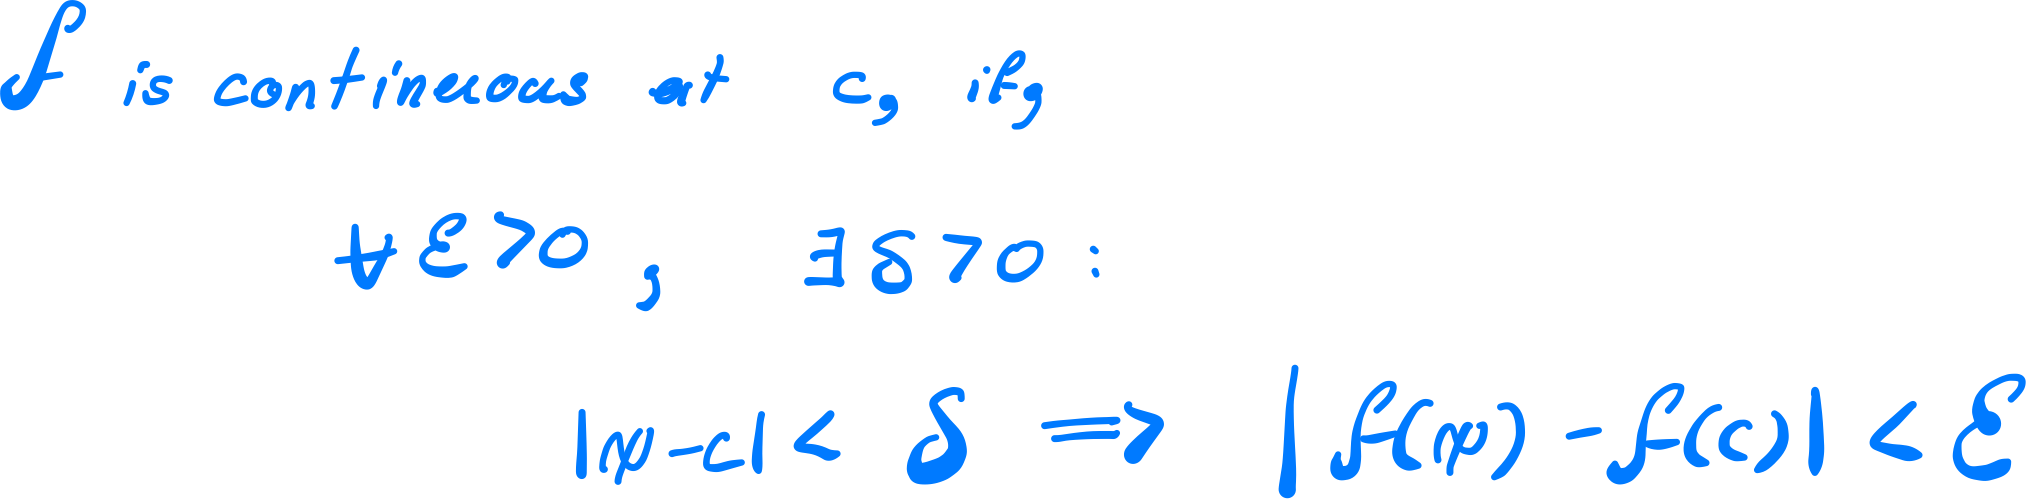
\includegraphics[width=0.7\textwidth]{media/Continuity/5a4384a9f2a06610556cce9d4252fedc2d5050eb.png}
\caption{TODO}
\end{figure}

\paragraph{Rigorous Definition}

So let's phrase that using the \(\varepsilon\)-\(\delta\) definition of
the limit: \\

\subparagraph{In Terms of Neighborhoods}

This can be expressed in terms of neighborhoods:
\begin{figure}
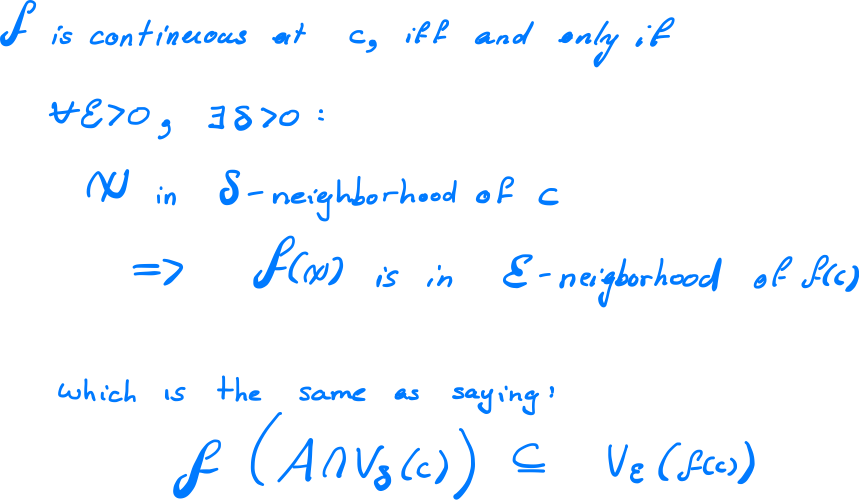
\includegraphics[width=0.7\textwidth]{media/Continuity/6d89890c4876af9738ff2bd73575f425a45c101a.png}
\caption{Notes from the iPad, TODO transcribe}
\end{figure}

\newpage
\hypertarget{header-n3893}{%
\paragraph{Conditions for Continuity}\label{header-n3893}}

If \(c\) is a cluster point of \(A\), then trhee conditions must hold
for \(f\) to be continuous at \(c\), that is to say that three
conditions must hold for \(\lim_{x\rightarrow c} = f(c)\):

\begin{enumerate}
\def\labelenumi{\arabic{enumi}.}
\item
  \(f\) must be defined at \(c\)

  \begin{itemize}
  \item
    so that \(f(c)\) actually has meaning
  \end{itemize}
\item
  The limit of \(f\) at \(c\) must exist in \(\mathbb{R}\) so that

  \begin{itemize}
  \item
    \(\lim_{x\rightarrow c}\) actually has a meaning
  \end{itemize}
\item
  These two values are equal

  \begin{itemize}
  \item
    \(\lim_{x\rightarrow c} = f(c)\)
  \end{itemize}
\end{enumerate}

\begin{quote}
\textbf{\emph{Cluster Points}}

A cluster point has infinitely divisible values either side of it, if a
value is not a cluster point it's just an isolated point and it is said
to be continuous at that point, so generally we just assume points are
cluster points because if they're not then they're automatically
continuous and so not very interesting.
\end{quote}

\hypertarget{header-n3914}{%
\subsubsection{Sequential Criterion for Continuity
{[}5.1.3{]}}\label{header-n3914}}

Just like a limits can be defined in terms of sequences (at (4.1.8) of
the TB), continuity can hence be defined in terms of sequences:

A function \(f: A \rightarrow \mathbb{R}\) is continuous at some point
\(c \in A \) if and only if:

\begin{itemize}
\item
  for every sequence \((x_n)\) in \(A\) that converges to \(c\)

  \begin{itemize}
  \item
    \(f\left(\left( x_n \right) \right)\) converges to \(c\) 
  \end{itemize}
\end{itemize}

\hypertarget{header-n3923}{%
\paragraph{Discontinuity Criterion {[}5.1.4{]}}\label{header-n3923}}

Just like limits can have divergence criteria in terms of limits, so can
the continuity definition, this is analogous to the \emph{Limit
Divergence Criteria} at (4.1.9(a) of the TB).

A function \(f: A \rightarrow \mathbb{R}\) is \textbf{discontinuous} at
some point \(c \in A \) if and only if:

\begin{itemize}
\item
  there exists some sequence \((x_n)\) in \(A\) that converges to \(c\):

  \begin{itemize}
  \item
    \(f\left(\left( x_n \right) \right)\) \emph{*does note} converge to
    \(c\) 
  \end{itemize}
\end{itemize}

\hypertarget{header-n3932}{%
\subparagraph{Example}\label{header-n3932}}

\(\lim_{x\rightarrow 0} \sin(\frac{1}{x^2})\) is undefined, so a
sequence that converges to 0 does is such that
\(f\left(\left( x_n \right) \right)\) \emph{*does note} converge to
\(c\) and so by (5.1.4) we can conclude that the function is
discontinuous at 0.

\hypertarget{header-n3934}{%
\subsubsection{Set Continuity}\label{header-n3934}}

if \(B\) is a subset of \(A\) we can say that the function
\(f: A \rightarrow B \) is continuous on \(B\) if it is continuous at
every point on \(B\).

\hypertarget{header-n3936}{%
\subsubsection{Defining a function to overcome
Discontinuity}\label{header-n3936}}

So take a function that is discontinuous, e.g.
\(\enspace f(x) = \frac{x^2-1^2}{(x+1)\cdot (x-1)}\) is discontinuous at
\(x = \pm 1\), to overcome this we can define a anew function \(g(x)\):

\[g(x) = 
  \begin{cases}
    f\left( x \right) , \enspace
   x\neq \pm1\\ 
   1\quad \enspace \enspace  , \enspace   x = \pm 1\\
      \end{cases}\]

This function will be continuous because the 'hole' is more or less
'plugged' by a given value.

\begin{itemize}
\item
  if there is no limit value at the discontinuity, then obviously this
  method won't work because we have no value with which to 'plug' the
  'hole'
\end{itemize}

\hypertarget{header-n3943}{%
\subsection{Combinations of Continuous Functions
{[}5.2{]}}\label{header-n3943}}

\hypertarget{header-n3944}{%
\subsubsection{Absolute Values Preserve Continuity
(5.2.4)}\label{header-n3944}}

Take our function \(f: A \rightarrow B\) and define the absolute
function as :

\begin{itemize}
\item
  \(\text{abs}(f)(x) = \left| f \right|(x) := \left| f(x) \right| \qquad\forall x \in A\)

  \begin{itemize}
  \item
    If \(f\) is continuous at \(c\), then \(\left| f(x) \right|\) is
    continuous at \(c\) 
  \item
    If \(f\) is continuous on \(A\), then \(\left| f(x) \right|\) is
    continuous on \(A\) 
  \end{itemize}
\end{itemize}

\hypertarget{header-n3954}{%
\subsubsection{Square Roots Preserve Continuity}\label{header-n3954}}

Take our function \(f: A \rightarrow B\) and define the square root
function as :

\begin{itemize}
\item
  \(\text{sqrt}(f)(x) = \left(\sqrt{(f)}\right) \left(x\right) := \sqrt{f(x)} \qquad\forall x \in A\)

  \begin{itemize}
  \item
    If \(f\) is continuous at \(c\), then
    \( \left(\sqrt{(f)}\right) \left(x\right)\) is continuous at \(c\) 
  \item
    If \(f\) is continuous on \(A\), then
    \( \left(\sqrt{(f)}\right) \left(x\right)\) is continuous on \(A\) 
  \end{itemize}
\end{itemize}

\hypertarget{header-n3964}{%
\subsubsection{Compositions Preserve Continuity}\label{header-n3964}}

Let:

\begin{itemize}
\item
  \(A, B \subseteq R\)

  \begin{itemize}
  \item
    \(f: A \rightarrow B\) 
  \item
    \(g: B\rightarrow \mathbb{R}\)

    \begin{itemize}
    \item
      \(f(A) \subseteq \mathbb{R}\) 
    \end{itemize}
  \end{itemize}
\end{itemize}

If \(f\) is continuous at \(c\) and \(g\) continuous at \(f(c)\) then
\(g\left( f\left( x\right) \right) = \left(g \circ f \right): A \rightarrow \mathbb{R}\)
is continuous at \(c\)

If \(f\) is continuous on \(A\) and \(g\) continuous on \(B\) then
\(g\left( f\left( x\right) \right) = \left(g \circ f \right): A \rightarrow \mathbb{R}\)
is continuous on \(A\)

\hypertarget{header-n3979}{%
\subsection{Continuous Functions on Intervals
{[}5.3{]}}\label{header-n3979}}

These weren't in the lecture Notes, they're probably not too important.

\hypertarget{header-n3981}{%
\subsection{Uniform continuity {[}5.4{]}}\label{header-n3981}}

These weren't in the lecture Notes, they're probably not too important.

\hypertarget{header-n3984}{%
\subsection{The Mean Value Theorem {[}6.2{]}}\label{header-n3984}}

\hypertarget{header-n3985}{%
\subsubsection{Maximum / Minimum {[}6.2.0{]}}\label{header-n3985}}

Take some function \(f: I \rightarrow \mathbb{R}\)

\begin{itemize}
\item
  \(f\) has a relative \textbf{maximum} if there exists some
  neighbourhood \(V:=V_{\delta}\left( c \right)\) such that::

  \begin{itemize}
  \item
    \(f(x) \geq f(c) \quad \forall x \in \left( V\cap I \right)\)
  \end{itemize}
\item
  \(f\) has a relative \textbf{minimum} if there exists some
  neighbourhood \(V:=V_{\delta}\left( c \right)\) such that:

  \begin{itemize}
  \item
    \(f(x) \leq f(c) \quad \forall x \in \left( V\cap I \right)\)
  \end{itemize}
\end{itemize}

If either of these are satisfied then \(f\) is said to have a
\textbf{relative extrema}

\hypertarget{header-n3999}{%
\subsubsection{Interior Extrema Theorem
{[}6.2.1{]}}\label{header-n3999}}

let \(c\) be a point on some interval \(I\) at which \(f\) has a max/min

\begin{itemize}
\item
  If there is a derivative at \(c\) then it must be 0:

  \begin{itemize}
  \item
    \(c\) is a point of at which \(f\) has a \emph{relative extremum}
    \(\implies\) \(f^{\prime}(c)=0\)
  \end{itemize}
\item
  The derivative at \(c\) must be 0 or must be undefined.

  \begin{itemize}
  \item
    \(f'(c) = 0 \vee f'(c) \in \emptyset\)
  \item
    \(f'(c) = 0 \vee f'(c) \downarrow\)
  \end{itemize}
\end{itemize}

In \emph{Computability: An Introduction to Recursion Theory} 1 the
\(\downarrow\) symbol is said to mean undefined, it's a useful notation
so I've adopted it, \(\in \emptyset\) is potentially another technique
as well.

\newpage
\hypertarget{header-n4017}{%
\subsubsection{Rolle's Theorem {[}6.2.3{]}}\label{header-n4017}}

Suppose that:

\begin{itemize}
\item
  \(f\) is continuous on \(I:= [a,b]\)
\item
  \(f'\) exists at every point of the open interval \((a,b)\)
\item
  \(f(a) = f(b) = 0\)
\end{itemize}

Then there must exist some value \(c\) such that \(f'(c) = 0\)

\begin{itemize}
\item
  This is the same as saying there must be a point of relative extrema
  (by the \emph{Interior Extrema Theorem})
\end{itemize}

\begin{figure}
\centering
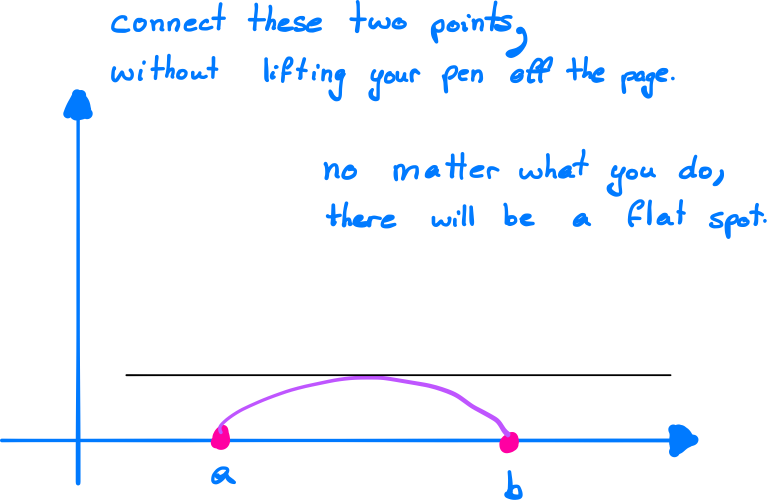
\includegraphics[width=0.7\columnwidth]{media/Continuity/f90f9756a7cc0b3ce971b414fb96a5f04d7c53dd.png}
\caption{}
\end{figure}

\begin{figure}
\centering
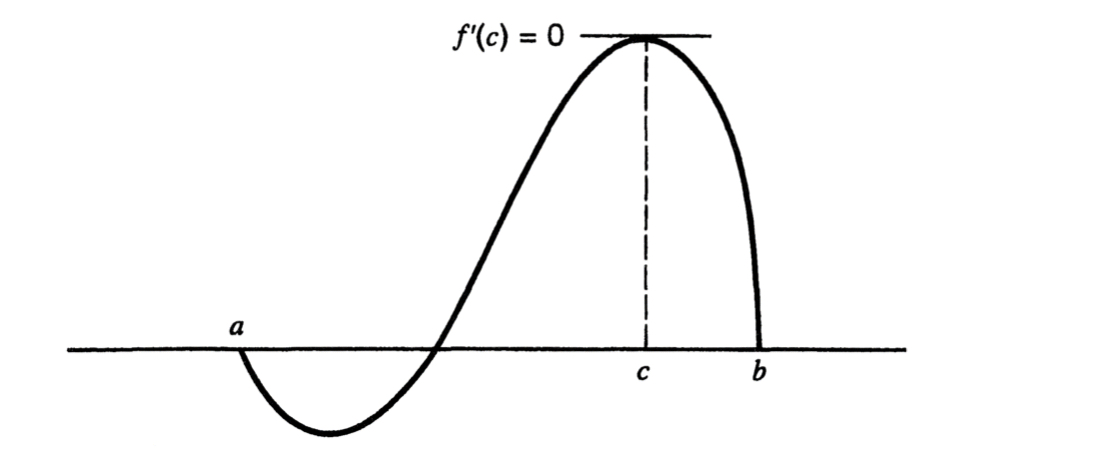
\includegraphics[width=0.7\textwidth]{media/Continuity/E744A1A9-00E0-4C46-971D-CE0A063D7664.jpeg}
\caption{}
\end{figure}

\hypertarget{header-n4032}{%
\subsubsection{Mean Value Theorem {[}6.2.4{]} }\label{header-n4032}}

This is basically a built up version of Rolle's Theorem,

Suppose that:

\begin{itemize}
\item
  \(f\) is continuous on \(I:= [a,b]\)
\item
  \(f'\) exists at every point of the open interval \((a,b)\)
\end{itemize}

Then, there must exist some \(c\):

\[f'\left( c \right) = \frac{f\left( b \right)-f\left( a \right)}{b-a} \\
\implies  \left( b-a \right) \cdot f\left( c \right) = f\left( b \right) - f\left( a \right)\]

\begin{figure}
\centering
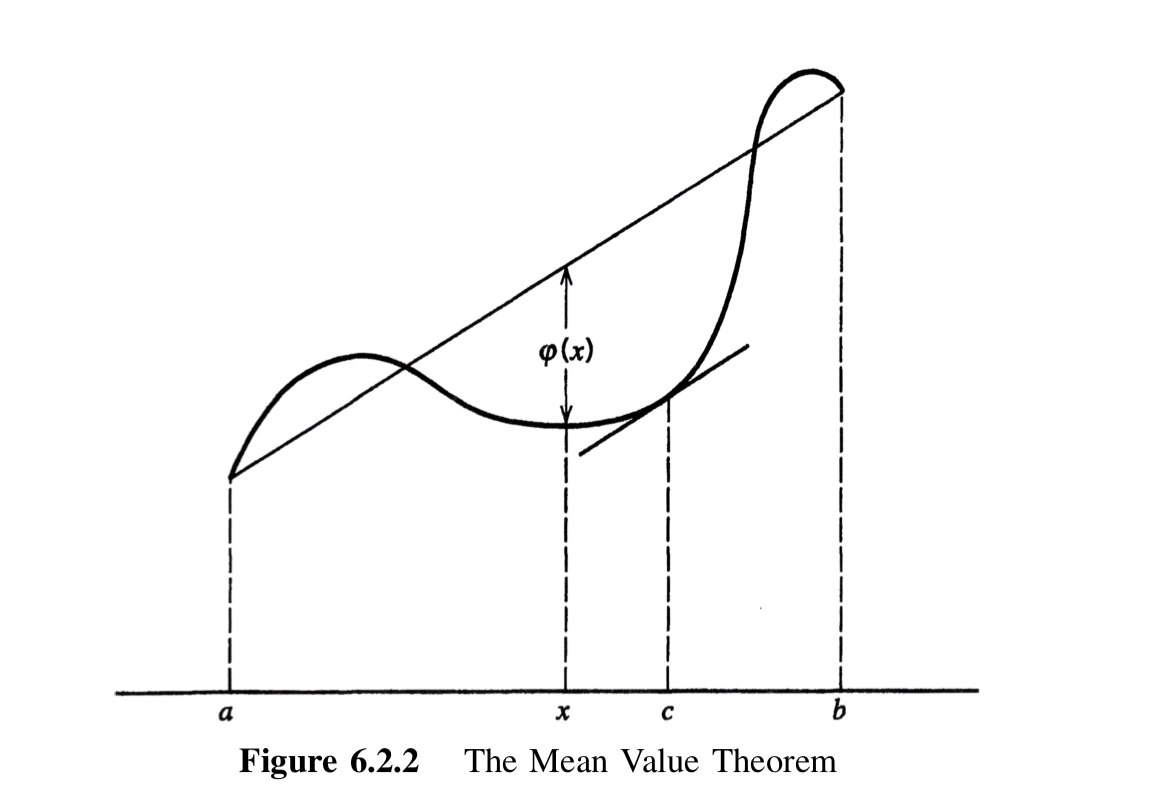
\includegraphics[width=0.7\columnwidth]{media/Continuity/3256156E-84DC-4942-B3D3-B580180EEE50.jpeg}
\caption{}
\end{figure}

\newpage
\hypertarget{header-n4043}{%
\subsection{L'Hospital's Rules}\label{header-n4043}}

\hypertarget{header-n4044}{%
\subsubsection{Cauchy Mean Value Theorem}\label{header-n4044}}

let \(f\) and \(g\) be:

\begin{itemize}
\item
  Continuous on {[}a,b{]}
\item
  Differentiable on (a,b)
\end{itemize}

if \(g'(x)  \neq 0\) , then \(\exists c \in (a,b)\) :

\[\frac{f\left( b \right)-f\left( a \right)}{g\left( b \right) - g\left( a \right)} = \frac{f'\left( c \right)}{g'\left( c \right)}\]

\hypertarget{header-n4054}{%
\paragraph{Restrictions}\label{header-n4054}}

By \emph{Rolle's Theorem}, if \(g'(x) \neq 0\), then \(g(a) \neq g(b)\).

\hypertarget{header-n4056}{%
\subparagraph{Creating a stricter restriction}\label{header-n4056}}

Let's suppose for some reason you needed to create the restriction:

\begin{itemize}
\item
  \(g'(x) \neq 0\), and
\item
  \(g(a) \neq g(b)\) 
\end{itemize}

An equivalent restriction would be:

\[\left( f'\left( x \right) \right)^{2} + \left( g'\left( x \right) \right)^{2} \neq 0\]


\end{document}

 %\documentclass{article}
\usepackage{amsmath}
\usepackage{amssymb}
\begin{document}
Let $X: = \left( x_n \right)$ and $Y:= \left( y_n \right)$ by sequences in $\mathbb{R}$ and let the partial sums of $\sum\left( y_n \right)$ be denoted by $\left( s_)n \right)$ with $s_0 : = 0$ \\

If $m>n$, then

\begin{equation}
  \sum_{k=n+1}^{m}\left[ x_ky_k \right]=\left( x_ms_m - x_{n+1}s_n \right) + \sum{k=n+1}^{m-1}\left( x_k-x_k+1 \right)s_k
  \label{partsum}
\end{equation}


$v:=v_{\delta}\left( c \right)$

$f'\left( c \right) = \frac{f\left( b \right)-f\left( a \right)}{b-a}$
\left( b-a \right) \cdot f\left( c \right) = f\left( b \right) - f\left( a \right)


\frac{f\left( b \right)-f\left( a \right)}{g\left( b \right) - g\left( a \right)} = \frac{f'\left( c \right)}{g'\left( c \right)}

\end{document}


 %
 \chapter{Complex Values}
 % Options for packages loaded elsewhere
%
\documentclass[class=article, crop=false]{standalone}

\usepackage{./resources/style}
\usepackage{./resources/referencing}

\usepackage{lmodern}
\usepackage{amssymb,amsmath,esint}
\usepackage{ifxetex,ifluatex}
\ifnum 0\ifxetex 1\fi\ifluatex 1\fi=0 % if pdftex
  \usepackage[T1]{fontenc}
  \usepackage[utf8]{inputenc}
  \usepackage{textcomp} % provide euro and other symbols
\else % if luatex or xetex
  \usepackage{unicode-math}
  \defaultfontfeatures{Scale=MatchLowercase}
  \defaultfontfeatures[\rmfamily]{Ligatures=TeX,Scale=1}
\fi
% Use upquote if available, for straight quotes in verbatim environments
\IfFileExists{upquote.sty}{\usepackage{upquote}}{}
\IfFileExists{microtype.sty}{% use microtype if available
  \usepackage[]{microtype}
  \UseMicrotypeSet[protrusion]{basicmath} % disable protrusion for tt fonts
}{}
\makeatletter
\@ifundefined{KOMAClassName}{% if non-KOMA class
  \IfFileExists{parskip.sty}{%
    \usepackage{parskip}
  }{% else
    \setlength{\parindent}{0pt}
    \setlength{\parskip}{6pt plus 2pt minus 1pt}}
}{% if KOMA class
  \KOMAoptions{parskip=half}}
\makeatother
\usepackage{xcolor}
\IfFileExists{xurl.sty}{\usepackage{xurl}}{} % add URL line breaks if available
\IfFileExists{bookmark.sty}{\usepackage{bookmark}}{\usepackage{hyperref}}
\hypersetup{
  hidelinks,
  pdfcreator={LaTeX via pandoc}}
\urlstyle{same} % disable monospaced font for URLs
\setlength{\emergencystretch}{3em} % prevent overfull lines
\providecommand{\tightlist}{%
  \setlength{\itemsep}{0pt}\setlength{\parskip}{0pt}}
\setcounter{secnumdepth}{-\maxdimen} % remove section numbering
\ifluatex
  \usepackage{selnolig}  % disable illegal ligatures
\fi

\author{}
\date{}

\begin{document}

\hypertarget{integrals-from-a-real-domain}{%
\section{Integrals from a Real
Domain}\label{integrals-from-a-real-domain}}

To begin this consider the function: \[
w: \mathbb{R}     \rightarrow \mathbb{C}
\] we can decompose such a function into real and imaginary components:
\[
w \left( t \right) =  u \left( t \right) +  i \cdot  v \left( t \right)
\] where \(u\) and \(v\) are purely real functions.

\hypertarget{differentiation}{%
\subsection{Differentiation}\label{differentiation}}

If \(w = f \left( z \right)\): \[
f' \left( z \right) = \frac{\operatorname{d}w }{\operatorname{d} z} \quad \text{(As if $z$ was a purely real operator)}
\] If
\(g\left( x,y \right) = u\left( x,y \right) + i \cdot v \left( x, y \right)\):

\[
\begin{aligned}
        f'\left( z \right) &= \frac{\partial u }{\partial x}+ \frac{\partial v }{\partial x} \\
        &= \frac{dw}{dz}
        \end{aligned}
        \]

If \(w = u\left( t \right) + i \cdot v \left( t \right)\): \[
w'\left( t \right) =  \frac{\operatorname{d}u }{\operatorname{d} t} + i \cdot \frac{\operatorname{d} v}{\operatorname{d} t}
\]

\hypertarget{integration}{%
\subsection{Integration}\label{integration}}

If \(w = u\left( t \right) + i \cdot v \left( t \right)\):

\[
\int^{b}_{a}\left( w \left( t \right)  \right) \operatorname{d}t =  \int^{b}_{a}\left( u \right) \operatorname{d}t + i \cdot  \int^{ b}_{a}\left( v \right) \operatorname{d}t
\]

\hypertarget{fundamental-theorem-of-calculus}{%
\paragraph{Fundamental Theorem of
Calculus}\label{fundamental-theorem-of-calculus}}

~\\
The fundamental theorem of calculus applies here: \[
\begin{aligned}
         \int^{b}_{a}\left( w\left( t \right)  \right) \operatorname{d}t =  \left[ W\left( t \right)  \right]^b_a 
          \label{ftcest}
        \end{aligned}
        \]

\hypertarget{justification}{%
\subparagraph{Justification}\label{justification}}

let
\(W\left( t \right) = U\left( t \right) + i \cdot V\left( t \right)\) be
the antiderivative of \(w\left( t \right)\):

\[
\begin{aligned}
          \int^{b}_{a}\left( w \left( t \right)  \right) \operatorname{d}t &= \left[ U\left( t \right)  \right]^b_a + i\cdot \left[ v\left( t \right)  \right]^b_a \\
          &= \left[ U\left( b \right) + i\cdot V\left( b \right)  \right] -\left[ U\left( a \right) +  i \cdot V\left( a \right)  \right]  \\
          &= \left[ W\left( b \right) - W\left( a \right)  \right] \\
          &= \left[ W\left( t \right)  \right]^b_a
        \end{aligned}
        \]

\begin{center}\rule{0.5\linewidth}{0.5pt}\end{center}

\hypertarget{contours}{%
\section{Contours}\label{contours}}

Integrals of complex valued functions are of the form:
\[\lim_{n     \rightarrow \infty}\left( \sum^{n}_{i= 1}\left[ f\left( z^*_i \right) \cdot \Delta z \right]  \right)\]
\(\Delta z\) could be along any curve in the complex plane rather than
just the axis along which we would integrate:

this short curve is what we call a contour, the complex integral will be
a line integral along that curve:

\hypertarget{define-contours}{%
\paragraph{Define Contours}\label{define-contours}}

~\\
A set of points \(z = \left( x,y \right)\) in the complex plane is said
to be an \textbf{\emph{arc}} or a curve that we will call \(C\) if:

\[\begin{aligned}
 x =  x\left( t \right), \quad y =  y\left( t \right) \qquad \left( a \leq t \leq b \right)
  \label{arcdef}\end{aligned}\]

where:

\begin{itemize}
\item
  \(x\left( t \right)\) and \(y\left( t \right)\) are continuous
  functions continuous however does not mean smooth/differentiable,
  sharp points are allowed.
\item
  the output values are ordered corresponding to \(t\) (as if \(t\)
  represented time)
\end{itemize}

It is more convenient to describe the curve at
(\protect\hyperlink{arcdef}{{[}arcdef{]}}) as:

\[\begin{aligned}
  z &= z\left( t \right)  \label{arccompdef} \\
  &= x\left( t \right) + i\cdot y\left( t \right) \notag\end{aligned}\]

\hypertarget{types-of-arcs}{%
\subparagraph{Types of Arcs}\label{types-of-arcs}}

~\\

\begin{itemize}
\item
  A \textbf{Simple Curve} does not cross itself
\item
  a \textbf{Closed Curve} meets back up with itself
\item
  a \textbf{Simple Closed Curve} is closed and does not cross itself
  (except where it closes)
\item
  a \textbf{Positive Curve} moves counter-clockwise as \(t\) increases.
\end{itemize}

\hypertarget{parametric-representation-not-unique}{%
\subparagraph{Parametric Representation not
unique}\label{parametric-representation-not-unique}}

~\\
Also the parametric representation of such a curve is not unique, the
same curve could be represented by lots of different parametric
equations, just like a second degree polynomial can also be modelled by
a 3rd degree polynomial between intervals.

\hypertarget{contour-integral}{%
\section{Contour Integral}\label{contour-integral}}

As previously discussed, an integral with respect to \(z\) will be a
contour integral: \[\int^{}_{C} f \left(z \right)   \operatorname{d}z\]
If the value of the integral does not depend on the path of the contour
and only depends on the endpoints then we would write:

\[\int^{}_{C} f \left(z \right)   \operatorname{d}z = \int^{z_2}_{z_1} f\left( z   \right) \operatorname{d}z\]
We can also put the integral in terms of the contour parameters, This is
basically \emph{Integration by Substitution} in reverse, there's a more
rigorous proof in the textbook by \emph{Osbourne}, just take it as
definition.

\[\begin{aligned}
    \int^{}_{C}\left( f\left( z \right)  \right) \operatorname{d}z = \int^{b}_{a}\left(f \left[ z\left( t \right)  \right]\cdot  z'\left( t \right)  \right) \operatorname{d}t  
    \label{tdef}
  \end{aligned}\]

\hypertarget{negative-contours}{%
\paragraph{Negative Contours}\label{negative-contours}}

~\\
If a contour \(C\) is given the contour \(- C\) denotes the same contour
with the order of the points reversed. Hence we have:

\[\begin{aligned}
     \int^{}_{-C}\left( f\left( z \right)  \right) \operatorname{d}z  &= \int^{- a}_{- b}\left( f\left[ z\left( - t \right)  \right] \cdot \frac{\operatorname{d} }{\operatorname{d} t}\left( z\left( - t \right)  \right)  \right) \operatorname{d}t \\
    &= - \int^{b}_{a}\left( f\left[ z\left( - t \right)  \right] z'\left( - t \right)  \right) \operatorname{d}t \\
    &= - \int^{}_{C}\left( f\left( z \right)  \right) \operatorname{d}z \end{aligned}\]

Refer to p.~128 of \emph{Churchill's 9th} for worked examples.

\hypertarget{notation}{%
\subsection{Notation}\label{notation}}

If we want to basically i want to know does the symbol:
\[\oint^{}_{} f\left( z \right)   \operatorname{d}z\]

\begin{itemize}
\item
  a contour/line integral of any sort
\item
  a contour/line integral around a closed path
\item
  one of the above but specifically in the anticlockwise direction?
\end{itemize}

\hypertarget{upper-bounds-for-moduli}{%
\subsection{Upper Bounds for Moduli}\label{upper-bounds-for-moduli}}

Start with the triangle inequality:
\[\left| \alpha + \beta \right| \leq     \left| \alpha \right| +     \left| \beta \right|\]
We could prove this, or, by similar reasoning:

Now let:

\begin{itemize}
\item
  \(C\) be a contour of length \(L\)
\item
  \(\left| f\left( z \right) \right| \leq M\)
\end{itemize}

Using the inequality above it can be rigorously shown:

\[\left| \int^{}_{}\left( f\left( z \right)  \right) \operatorname{d}z  \right| \leq M\cdot L\]

This can be somewhat visualised if \(f\left( z \right)\) is taken to be
the height of the function along the contour, and \(L\) is taken to be
the length of the contour, although the values will be complex and
height might become an odd concept, the mathematics should still hold.

\hypertarget{example}{%
\paragraph{Example}\label{example}}

Evaluate the contour integral:
\[\int^{}_{C}\left( \frac{1}{z} \right) \operatorname{d}z\] Where:

\begin{itemize}
\item
  \(C: \left| z \right| = 1\)
\item
  For the sake of argument, we say that the circle joins at
  \(z = -1 = \operatorname{cis} {\pi} = e^{\pi \cdot i}\)
\end{itemize}

Now put the integral in terms of the parametric representation
(\protect\hyperlink{tdef}{{[}tdef{]}}):

\[\begin{aligned}
       \int^{}_{C}\left( \frac{1}{z} \right) \operatorname{d}z &=  \int^{\pi}_{\pi}\left( \frac{1}{e^{i\theta}} \cdot \frac{\operatorname{d} }{\operatorname{d} \theta}\left( e^{i\theta} \right)  \right) \operatorname{d}\theta \notag \\
       &= \int^{\pi}_{\pi}\left( \frac{1}{e^{i\theta}} \cdot i\cdot e^{i\theta} \right) \operatorname{d}\theta \notag \\
       &= \int^{\pi}_{\pi}\left( i \right) \operatorname{d}\theta \notag \\  
       &= \left[ i \cdot \theta \right]^{\pi}_{\pi} \notag \\
       &= 0
     \label{excontint1}
   \end{aligned}\]

\hypertarget{antiderivatives}{%
\section{Antiderivatives}\label{antiderivatives}}

Generally the value of a contour integral depends on both the path of
the contour and the function.\\
Some contour intergrals however have values independent of the path, for
example consider how many integrals over closed paths will have an
integral of zero as in the example above.\\
The antiderivative of a complex function is \(F\left( z \right)\) such
that: \[F'\left( z \right) = f\left( z \right)\] The antiderivative is,
of necessity, an analytic function.

The antiderivative is uniqe, there is only one antiderivative for a
given funciton (other than the additive constant \(\left( + C \right)\)
component).

\hypertarget{basic-antiderivative-theorem}{%
\subsection{Basic Antiderivative
Theorem}\label{basic-antiderivative-theorem}}

Suppose \(f\left( z \right)\) is continuous in a domain, if the function
has an antiderivative \(F\left( z \right)\) through the domain then:

~~

integrals of \(f\left( z \right)\) along contours lying in the domain
depend only on the endpoints of that contour:
\[\int^{}_{C}f\left( z \right)  \operatorname{d}z = \int^{z_2}_{z_1} f\left( z \right)   \operatorname{d}z = \left[ F\left( z \right)  \right]^{z_2}_{z_1}\]

This also means that integrals around a closed contour will be 0.

~~

\hypertarget{proof}{%
\paragraph{Proof}\label{proof}}

if \(F'\left( z \right) = f\left( z \right)\) :

\begin{align*}
       \int^{}_{C} f\left( z \right)   \operatorname{d}z &=  \int^{b}_{a} f\left( z\left( t \right)  \right)   \operatorname{d}t \\
       &= \int^{b}_{a} U\left( z\left( t \right)  \right)   \operatorname{d}t + i\cdot \int^{b}_{a} b\left( z\left( t \right)  \right)   \operatorname{d}t\\
       \intertext{Which means the Fundamental Theorem of Calculus Applies from (\ref{ftcest})}
       &= F\left( z\left( b \right)  \right) - F\left( z\left( a \right)  \right) \\
       &=  F\left( z_2 \right) - F\left( z_1 \right) \\
       &= \left[ F\left( z \right)  \right]^{z_2}_{z_1} \\
       &= \left[ U\left( t \right)  \right]^{b}_{a} +  i \cdot  \left[ V\left( t \right)  \right]^{b}_{a} \\
       &= U\left( b \right) - U\left( a \right) +  i \cdot  \left[ V\left( b \right) - V\left( a \right)  \right] \\
       &= \left[ U\left( b \right)+  V\left( b   \right)  \right] -  i \cdot  \left[ U\left( a \right) - V\left( b \right)  \right] \\
       &= F\left( b \right) - F\left( a \right) \\
       &= \left[ F\left( z \right)  \right]^{b}_{a}\\
       &= \left[ F\left( z \right)  \right]^{z_2}_{z_1}
 \end{align*}

\hypertarget{cauchy-goursat-theorem}{%
\section{Cauchy Goursat Theorem}\label{cauchy-goursat-theorem}}

This theorem depends on \emph{Green's Theorem} which gives the
relationship between a line integral around a simple-closed curve and
the double integral over the corresponding bounded region, for purely
real functions. Roughly Speaking \emph{Green's Theorem} is a counterpart
of the Fundamental Theorem of Calculus for double integrals.\\
In establishing the \emph{Cauchy-Goursat Theorem}, proving \emph{Green's
Theorem} is the tricky part, the \emph{Cauchy-Goursat Theorem} more or
less falls out of it.

~~

\hypertarget{the-cauchy-goursat-theorem}{%
\subparagraph{\texorpdfstring{the \emph{Cauchy-Goursat
Theorem}}{the Cauchy-Goursat Theorem}}\label{the-cauchy-goursat-theorem}}

If a function \(f\) is analytic at all points interior to, and on, a
simple closed contour \(C\), then:

\[\oint^{}_{C} f\left( z \right)   \operatorname{d}z = 0\]

~~

\hypertarget{simply-connected-domains}{%
\subsection{Simply-Connected Domains}\label{simply-connected-domains}}

If \(f\left( z \right)\) is analytic through a simply connected domain:
\[\int^{}_{C} f\left( z \right)   \operatorname{d}z\] Where:

\begin{itemize}
\item
  C is any closed contour in that domain (Simple or not) i.e.~if the
  domain is simply connected, the contour can cross itself.
\end{itemize}

From this it follows:

\begin{itemize}
\item
  If a function is analytic on a simply connected domain, then: there
  will be an anti-derivative: The contour integral will be independent
  of path (i.e.\(F(b) - F(a)\)
\item
  Entire functions always have an antiderivative and will always be
  independent of path.
\end{itemize}

\hypertarget{multiply-connected-domains}{%
\subsection{Multiply Connected
Domains}\label{multiply-connected-domains}}

If \(C\) is a closed counter-clockwise contour, inside which are closed
Clockwise contours \(c_1, c_2, c_3 \dots\) for which the function is
analytic interior to C but exterior to \(c_1, c_2, c_3 \dots\) :

Then we have:

\[\int^{}_{C} f\left( z \right)   \operatorname{d}z + \sum^{k}_{n= 1} \left[ \int^{}_{c_n} f\left( z \right)   \operatorname{d}z  \right]\]
This is established by drawing a line through all the interior closed
contours and applying the \emph{Cauchy-Goursat} theorem, refer to the
\emph{Churchill} textbook.

\hypertarget{principle-of-deformation}{%
\paragraph{Principle of Deformation}\label{principle-of-deformation}}

If we had Something like this:

Then it would follow:

\[\begin{aligned}
  \int^{}_{C_1} f\left( z \right)   \operatorname{d}z + \int^{}_{c_2} f\left( z \right)   \operatorname{d}z &= 0\\  
  \int^{}_{C_1} f\left( z \right)   \operatorname{d}z - \int^{}_{c_2} f\left( z \right)   \operatorname{d}z &= 0\\
  \int^{}_{C_1} f\left( z \right)   \operatorname{d}z &= \int^{}_{c_2} f\left( z \right)   \operatorname{d}z  \end{aligned}\]

So if \(c_2\) can be continuously transformed into \(C_1\) through an
analytic region, then the integral is the same.

\hypertarget{spacial-case-of-deformation}{%
\subparagraph{Spacial Case of
Deformation}\label{spacial-case-of-deformation}}

We Should Probably memorise this special case:

\[\ointctrclockwise_{    \left| z - z_0 \right| = r} \left( z- z_0 \right) ^n  \operatorname{d}z =
\begin{cases}
  0 \qquad if n \neq - 1\\
  2\pi i \qquad if n = - 12
\end{cases}\]

\hypertarget{example-1}{%
\subparagraph{Example}\label{example-1}}

\begin{align*}
    \int^{}_{    \left| z \right| = 1} \frac{1}{z^2 +  2z+2 }  \operatorname{d}z &= \int^{}_{    \left| z \right| = 1} \frac{1}{\left( z +  \left( 1 +  i \right)  \right) \cdot \left( z +  \left( 1 -  i \right)  \right) }  \operatorname{d}z  \\
    \intertext{There is a singularity at $z =  - 1 \pm i$, which is outside the closed countour, the function is analytic everwhere else inside and on the closed countour hence by the \textit{Cauchy-Goursatt Theorem:}}\\
  \int^{}_{    \left| z \right| = 1} \frac{1}{z^2 +  2z +  2}  \operatorname{d}z &= 0 \end{align*}

\hypertarget{cauchy-integral-formula}{%
\section{Cauchy Integral Formula}\label{cauchy-integral-formula}}

This has to be memorised.~\\

\hypertarget{cauchy-integral-formula-1}{%
\subparagraph{Cauchy Integral Formula}\label{cauchy-integral-formula-1}}

~\\
If \(f\) is analytic everwhere inside and on \(C\) and \(z_0\) is
interior to C:
\[\int^{}_{C} \frac{f\left( z \right) }{z - z_0}  \operatorname{d}z = 2\pi i \cdot  f \left( z_0 \right)\]

~~

\hypertarget{example-2}{%
\paragraph{Example}\label{example-2}}

Solve :
\[\int^{}_{    \left| z \right| = 1} \frac{\cos{z}}{z^3 +  9z}   \operatorname{d}z\]
First simplify the intergrand somewhat:

\[\int^{}_{    \left| z \right| = 1} \frac{\cos{z}}{z^3 +  9z}  \operatorname{d}z = \int^{}_{    \left| z \right| = 1} \frac{1}{z} \cdot  \frac{\cos{z}}{z^2 +  9z}  \operatorname{d}z\]

Observe that the intergrand \(\frac{\cos{z}}{z^3 + 9z}\) is analytic
everywhere other than its singularities:

\begin{itemize}
\item
  \(z = 0\)
\item
  \(z = 3i\)
\item
  \(z = - 3i\)
\end{itemize}

because \(z = 0\) is inside the contour we cannot use the
\emph{Cauchy-Goursatt Theorem}, however, we can use the
\emph{Cauchy-Integral Formula} precisely because :

\begin{itemize}
\item
  \(z_0 = 0\) is interior to the closed contour
\item
  \(f\left( z \right) = \frac{\cos{z}}{z^2+ 9}\) is analytic everywhere
  else interior to the closed contour
\end{itemize}

So by the Cauchy Integral Formula:

\[\begin{aligned}
    \int^{}_{    \left| z \right| = 1} \frac{\frac{\cos{z}}{z^2+ 9}}{\left( z- 0 \right) }  \operatorname{d}z &= 2\pi i \cdot \frac{\cos{\left( 0 \right) }}{0^2+ 9} \\
    &= i\cdot \frac{2\pi}{9}\end{aligned}\]

\hypertarget{extension-of-the-cauchy-integral-formula}{%
\section{Extension of the Cauchy Integral
Formula}\label{extension-of-the-cauchy-integral-formula}}

This has to be memorised:

~~

\hypertarget{extension-to-cauchy-integral}{%
\subparagraph{Extension to Cauchy
Integral}\label{extension-to-cauchy-integral}}

~\\
if:

\begin{itemize}
\item
  \(f\left( z \right)\) is analytic on and interior to some closed
  contour \(C\)
\item
  \(z_0\) is interior to \(C\)
\end{itemize}

Then:
\[\int^{}_{C} \frac{f\left( z \right) }{\left( z- z_0 \right) ^{n+ 1}}  \operatorname{d}z = f^{n}\left( z_0 \right) \cdot \frac{2\pi i}{n!}\]

\end{document}


 \chapter{Complex Variables}
 \title{(08) Complex Variables}
\author{Ryan Greenup}
\date{Autumn 2019}

\documentclass[class=article, crop=false]{standalone}
\usepackage{./resources/style}

\begin{document}
	\maketitle
	\tableofcontents
	
	
	
\section{Functions of a Complex Variable}
A complex function is a function from a complex plane onto another complex + ane:
\begin{align*}
  A, B \subseteq \mathbb{C} &, \\
  & f: A \rightarrow B
\end{align*}

All the usual definitions of functions still apply, e.g.: 
\\ \

\hfill\begin{minipage}{\dimexpr\textwidth-3cm}
  \begin{itemize}
    \item Functions are rigourously defined using sets 
    \item There is a do main, range, codomain, image etc.
    \item $\dots$
  \end{itemize}
\end{minipage}
\\ \

The \textit{Churchill's} Textbook mentions these conventions however
\begin{enumerate}
  \item Usually the codomain is taken as the set of all complex values.
  \item Most of the results concerning real functions are taken as already established without justification
  \item $x, y, u, v$ denote real variables where as  $z$ and $w$ denote complex variables
    \subitem $z = x +  i y$ 
    \subitem w = u +  i v
    \subitem $f(z) = w \implies f\left( z \right) = u +  iv$
  \item Sometimes there won't be a clear distinction between the values of a function and the function itself, e.g.:
    \begin{align*}
      g\left( z \right) &=  z^2\\
      f\left( g\left( z \right) \right) &=  f\left( z^2 \right)  &\text{Here $z^2$ is shorthand for the function}
    \end{align*}
\end{enumerate}

\newpage
\section{Geometric Interpretation}
Imagine the real function $y = 3$ :
\begin{figure}[!h]
	\centering
	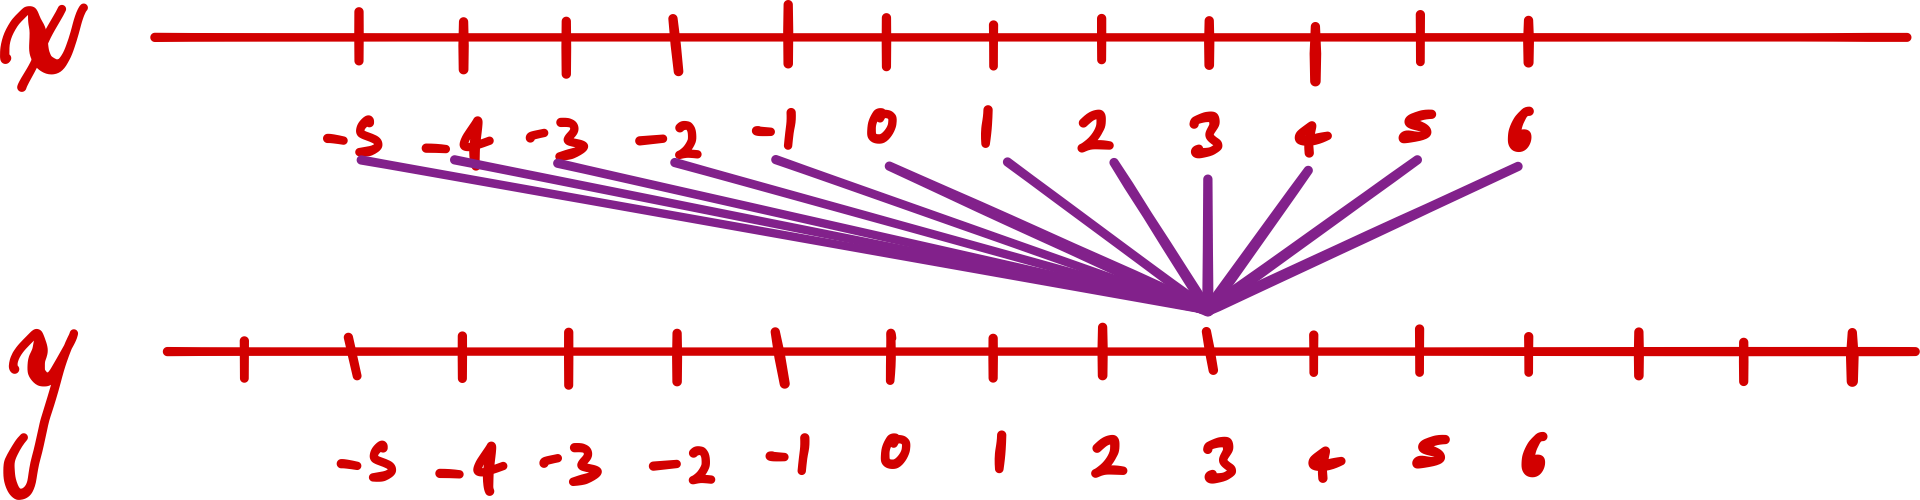
\includegraphics[width=0.7\linewidth]{"./media/ComplexFunctions/PNG image.png"}
	\caption{}
	\label{fig:png-image}
\end{figure}

A similar constant complex function would be $f\left( z \right) =  3 +  4i$:
\begin{figure}[h!]
	\centering
	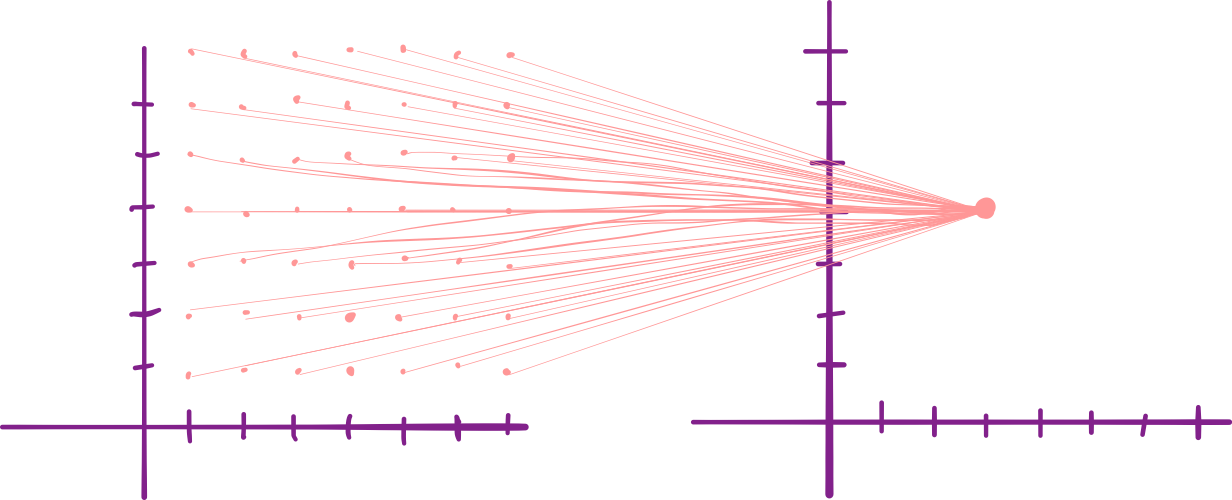
\includegraphics[width=0.7\linewidth]{"./media/ComplexFunctions/PNG image 2.png"}
	\caption{}
	\label{fig:png-image-2}
\end{figure}

It isn't possible to make a graph like it is with simple single variable real functions because that would require four spacial dimensions in order to plot it, this has the dissapointing consequence that geometric interpretations of derivatives as a slope and integrals as area beneath a curve are no longer helpful. \\

It isn't uncommon to use a 3D Cartesian plane to illustrate a function from the reals onto the complex, e.g. imagine $ y =  x^{2}$, if a complex domain is ullustrated as an $x$ /$y$ plane and a perpendicular $z$-axis represents the real codomain, the surface representing the values would always have two roots, even if the're not real, the \textit{Welch Labs} video \textit{Imaginary Numbers are real}\footnote{https://www.youtube.com/watch?v=T647CGsuOVU} is really good for getting a visualisation of this but the general visualisation is:


\begin{figure}[h!]
	\centering
	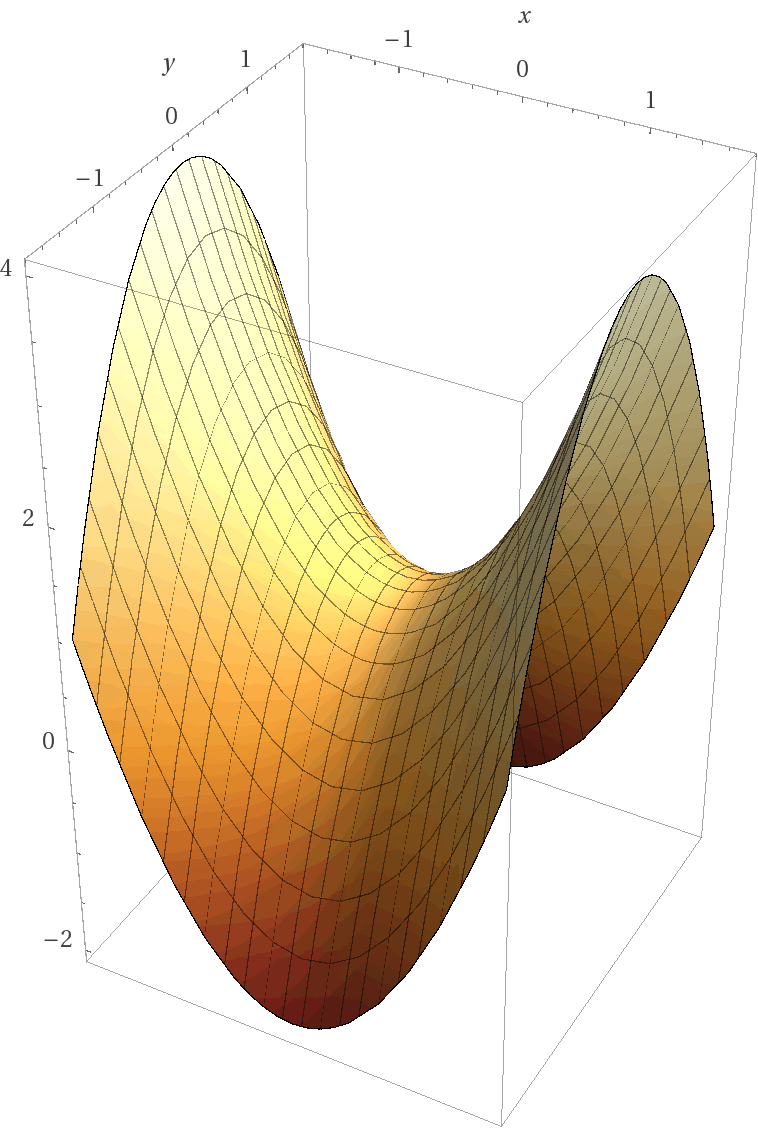
\includegraphics[width=0.2\linewidth]{"./media/ComplexFunctions/PNG image 3.png"}
        \caption{This can be generated in \textit{Wolfram} or something else by using $f(x,y) = \left( x +  i y \right)^2 +  1$}
	\label{fig:png-image-3}
\end{figure}


\section{Complex functions Components}
Complex functions can be illustrated as a pair of two-variable real functions.
Take a function:
\[
  f\left( z \right) =  w
\]
The $w$ variable can be expanded:

\[
  f\left( z \right) =  u +  iv
\]
the $z$ variable can also be expanded:
\[
  f\left( x +  i y  \right) =  u +  iv
\]
Observe that the value $ u$ is in essence a function of the $x$ and $y$ input variables, the same is true also for $v$,  hence, this can be rewritten:

\[
  f\left( x +  i y \right) =  u \left( x,y \right) +  i \times v\left( x,y \right)
  \]

\paragraph{Example}
\begin{align*}
  f\left( z \right) &= z^2 \\
  &= \left( x +  iy  \right)^{2} \\
  &=  x^2 - y^2 +  i \cdot 2xy \\
  &=  \left( x^2 - y^2  \right) +  i \cdot \left( 2xy \right)
  \intertext{So in this case the component functions would be:}
  u\left( x,y \right) &=  \left( x^2 -  y^2 \right) &&\text{and,}\\
  v\left( x,y \right) &=  \left( 2xy \right)
\end{align*}

Essentially a complex-valued function is a pair of two variable real functions.
\subsection{Limits}
if $f$ is defined on all poiints in a \textit{deleted neighbourhood} of $\alpha$ it is written:
\[
  \lim_{z \rightarrow \alpha}{f\left( z \right) = L}, \qquad \text{equivalently,} \qquad f\left( z \right) \rightarrow w_0 \text{\quad as \quad} z \rightarrow z_0.
\]
if and only if:


\hfill\begin{minipage}{\dimexpr\textwidth-3cm}
  $f\left( z \right)$ can be made arbitrarily close to $L$ by making $z$ sufficiently close to $\alpha$.
\end{minipage}
\\ \

In formal notation this is expressed:\\

\ \
\hfill\begin{minipage}{\dimexpr\textwidth-3cm}
\begin{tcolorbox}

  \subparagraph{Formal Definition of a Complex Limit}  \ \\
  \ \\
  If $f: A \rightarrow \mathbb{C} $ and $\alpha \in \overline{A}$ 
\begin{align*}
    \forall \varepsilon > 0, \enspace \exists \delta:& \\
    & 0 <     \left| z-\alpha \right| < \delta \implies     \left| f\left( z \right) - L \right| < \varepsilon
\end{align*}
\end{tcolorbox}

\end{minipage}
\\ \

\newpage 

\paragraph{Limits in Terms of Sequences}
A sequence of complex numbers $\left\{ z_n \right\}_{1}^{\infty}$ has a limit $z$ ( i.e. it converges to $z$) if:\\



\hfill\begin{minipage}{\dimexpr\textwidth-3cm}
\begin{tcolorbox}

  \subparagraph{Formal Definintion of a Limit to a Complex Sequence}
\begin{align*}
    \forall \varepsilon > 0, \enspace \exists N \in \mathbb{Z} :& \\
    i& n > N \implies     \left| z_n - z \right| < \varepsilon
\end{align*}
\end{tcolorbox}

\end{minipage}
\ \\

So this says, the limit of the sequence is $z$ iif the terms of the sequence can be made arbitrarily close to the limit value by moving sufficiently far along the sequence.\\


Limit values are unique, a function can only have a single limite value at a point (or no limit value if the limit is undefined at that point). \\


\paragraph{Limits from multiple directions}\ \\
A single variable real functions can only approach a variable from the left-hand side or the right-hand side, complex funcitons however can approach a varible along any curve in the complex plane. \\

So for example consider the limit of a function as  $z     \rightarrow 0$, $z$ could approach zero along:

\begin{itemize}
  \item the real-axis $\left( x, 0 \right) : x     \rightarrow 0 \implies z     \rightarrow 0$ 
  \item the imaginary-axis $\left( 0, y \right) : y     \rightarrow 0 \implies z     \rightarrow  0$
  \item any straight-line $y = mx : y     \rightarrow 0 \implies z     \rightarrow 0$
  \item along a parabola $y = x^2 : y     \rightarrow 0 \implies z     \rightarrow 0$
  \item any curve whatsoever at all\dots
\end{itemize}

What makes this more confusing is that a limit may approach a value along one curve but not another, maybe for example our function approaches $w = f \left( z \right) = L$ as the variable approaches 0 on both the  $x$-axis and the $y$-axis, despite this it's entirely possible that our function approaches the value 33 along a parabola, the value 42 along a straight line and maybe $6 \pi +  4i$ along a cubic curve. \\


So it's really worth noting that as a \textbf{necessary but not sufficient condition}, the limit taken along the axis must be equal in order for the limit to exist, if they are equal however, the limit is not guaranteed to exist, it may be another value along a different curve. It's worth reading \textit{Pauls Online Notes} \footnote{http://tutorial.math.lamar.edu/Classes/CalcIII/Limits.aspx}\\

The reason for often taking limits along the axis (as opposed to some other arbitrary curve), is because  the axis zeroes out a term which can be simpler and because the partial derivatives are also taken along the axis, which is used in developing the \textit{Cauchy Riemann} equations later, but, really, there is no difference taking the limit along arbitrary curves or along the axis, the function doesn't necessarily care. \\

\newpage 

\paragraph{Theorems on Limits}
The idea here is to establishh a connection between limits of complex functions and limits of real functions so we can use all the pre-established properties of real limits from calculus. \\


if:
\begin{align*}
z &=  x +  i y \\
f\left( z \right) &=  u\left( x, y \right) +  i \cdot  v \left( x, y  \right)
\end{align*}

Then we have:
\[
  \lim_{z \rightarrow \alpha} \left( f\left( z \right) \right) =  L
\]
if and only if:

\[
  \lim_{\left( x, y \right)     \rightarrow \left( a, b \right) }\left[ u \left( x, y \right)  \right] = \operatorname{Re}\left( L \right) \quad \text{and} \quad \lim_{\left( x, y \right)     \rightarrow \left( a,b \right) }\left[ v\left( x,y \right)  \right] = \operatorname{Im}\left( L \right) 
\]

So now we can break the complex limits up into real components that we already know how to deal with, and all the familiar \textit{Limit Laws} carry over from earlier calculus.

\paragraph{Limit Laws}

\subparagraph{Distribution over Addition}
\[
\lim_{z     \rightarrow z_0}\left[ f \left( z \right) g \left( z \right)  \right] =  \lim_{z     \rightarrow z_0}\left[ f \left( z \right)  \right] + \lim_{z     \rightarrow z_0}\left[ g \left( z \right)  \right] 
\]
\subparagraph{Distribution over Multiplication}
\[
\lim_{z     \rightarrow  z_0}\left[ f \left( z \right) \cdot g \left( z \right)  \right] = \lim_{z     \rightarrow  z_0}\left[ f \left( z \right)  \right] \cdot \lim_{z     \rightarrow  z_0}\left[ g \left( z \right)  \right] 
\]
\subparagraph{Distribution over Division}\ \\
Assume that $\lim_{z     \rightarrow  z_0}\left[ g \left( z \right)  \right] \neq 0$:
\[
  \lim_{z     \rightarrow  z_0}\left[ \frac{f \left( z \right) }{g \left( z \right) } \right] = \frac{\lim_{z     \rightarrow  z_0}\left[ f \left( z \right)  \right] }{\lim_{z     \rightarrow  z_0}\left[ g \left( z \right)  \right] }
\]



\paragraph{Riemann Sphere}
Limits at infinity are given a theoretical foundation using an idea called the \textit{Riemann Sphere}, it's interesting but a deep understanding of the theory isn't necessary in order to work with limits at infinity so dont worry about it.

\newpage

\section{Continuity}
A function $f$ is  \textit{continuous} at a point $z_0$ if for all points $\lim_{z     \rightarrow z_0}\left[ f \left( z \right)  \right] = f \left( z_0 \right) $.

This is generally broken up into three conditions for want of decomposing problems:\\


\hfill\begin{minipage}{\dimexpr\textwidth-3cm}
\begin{tcolorbox}

  \subparagraph{Conditions of Continuity}\ \\
  A function $f$ is \textit{Continuous} at $z_0$ if the following three conditions are all satisfied:
  \ \\
  \begin{enumerate}
    \item $\lim_{z     \rightarrow  z_0}\left[ f \left( z \right)  \right] $ \\
    \item $f \left( z_0 \right) $ exists \\
    \item $\lim_{z     \rightarrow   z_0}\left[ f \left( z \right)  \right] = f \left( z_0 \right) $ {\tiny (which implies the above 2)}
  \end{enumerate}
\end{tcolorbox}

\end{minipage}
\ \\




If a function is continuous on some neighbourhood, it's limit value for any point in that neighbourhood is the function value, this means, if we did, for instance, take the limit at a point along both axis (or along any two arbitrary curves), and they were equal, then the limit would be defined at that point, because it would be the function value.\\

If a function can be differentiated at a point, the function is continuous at that point. \\

So if we could show that a derivative exists on all points of some neighbourhood, and that the derivative was continuous at some point, then that neighbourhood would be continuous and the limit at that point would certainly exist. \\

\hfill\begin{minipage}{\dimexpr\textwidth-3cm}
This might seem a little bit contrived, but these are the pieces that are used for the \textit{Cauchy Riemann} equations 
\end{minipage}
\ \


\newpage


\paragraph{Function Composition}\ \\
A composition of continuous functions is continuous, e.g. \ \\
\ \\
if:
\begin{align*}
  f \left( x \right) &= x^2 \quad &\text{is continuous} \\
  g \left( x \right) &= e^x \quad &\text{is contninous}
\end{align*}
Then:
\begin{align*}
  f \circ g =  f \left[  g \left( x \right)  \right]  &=  e^{x^{2}} &\text{is continuous}
\end{align*}
\ \\
Again, this might seem obvious, but it's useful for complex functions and is necessary in the \textit{Cauchy Riemann} equations.


\subparagraph{Continuity of Complex Functions}
A Complex function is only continuous if the real two-variable components $u \left( x, y \right)$ and $v \left( x,y \right) $ are continuous:\\

\hfill\begin{minipage}{\dimexpr\textwidth-3cm}
  {\footnotesize This is because a composition of continuous functions is continuous}
\end{minipage}
\ \\

\begin{figure}[h!]
	\centering
	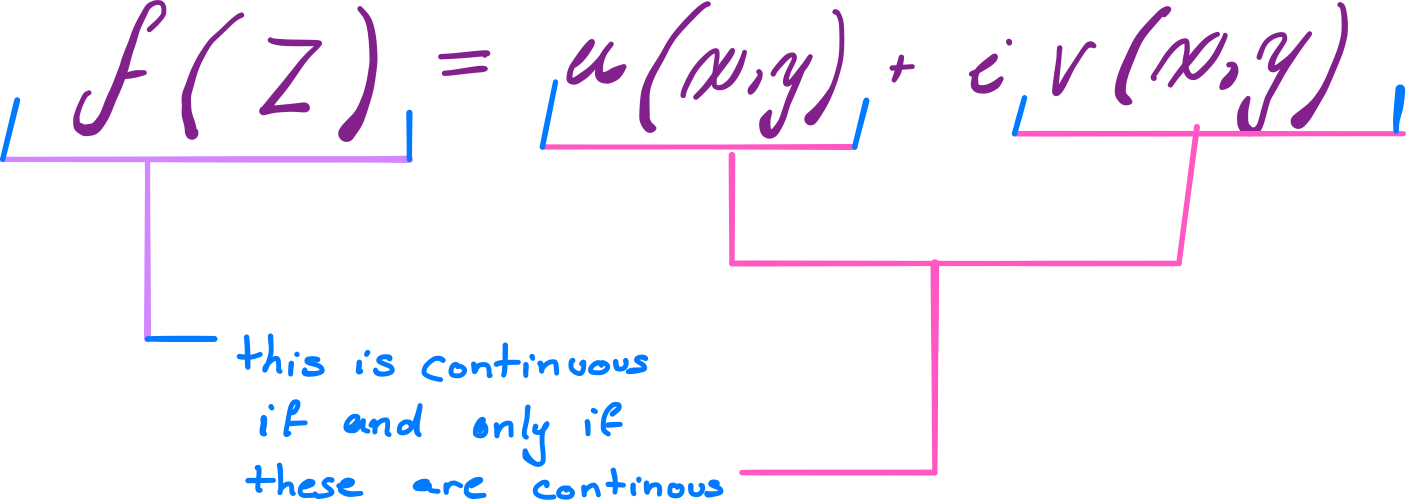
\includegraphics[width=0.7\linewidth]{"./media/ComplexFunctions/PNG image 4.png"}
%	\caption{}
	\label{fig:png-image-4}
\end{figure}

Again, remember this for later when we are doing the \textit{Cauchy Riemann} equations.


\newpage


\section{Derivatives}
Derivatives have the same definition in complex analysis as they do in real calculus, with the difference that the variable is now complex, the derivative of $f$ at $a$ is:

  \begin{align*}
    w &= f \left( z \right)\\
    &\implies \frac{\operatorname{d} w}{\operatorname{d} z} = \lim_{\Delta Z\rightarrow 0}\left[ \frac{\Delta w}{\Delta z} \right] 
  \end{align*}

Or in a more useful fashion:

\[
  f'\left( a \right) = \lim_{\Delta Z\rightarrow 0}\left[ \frac{f \left( z \right) - f \left( a \right) }{z - a} \right] = \lim_{\Delta Z\rightarrow 0}\left[ \frac{f \left( a + \Delta z \right) -  f \left( a \right) }{\Delta z} \right] 
\]

A function may be differentiable at a point $z$ but not necessarily at any other points in the neighbourhood of $z$. \\

The real and imaginary components of a function may have continuous partial derivatives (of all orders) yet this does not imply that the function is differentiable there, 

\ \

\hfill\begin{minipage}{\dimexpr\textwidth-3cm}
e.g.  $   f\left( z \right) =   \left| z \right|$ has continuous partial derivatives away from $z =  0$, but is not differentiable anywhere, because the limits as $\Delta   z  \rightarrow 0$ are different depending on which path is taken.\end{minipage}
\ \





\paragraph{Conditions of Continuity}
\begin{itemize}
  \item if a function is continuous it may or may not be differentiable
  \subitem continuity $ \centernot\implies $ differentiability
  \item if a function is differentiable it must be continuous
  \subitem differentiability $ \implies  $ continuity
\end{itemize}

\subsection{Derivatives to Memorise}
The following complex functions are nowhere differentiable:

\begin{itemize}
  \item $f\left( z \right)  = \Re{\left( z \right) }$ 
  \item $f\left( z \right) = \Im{\left( z \right) }  $ 
  \item $f\left( z \right)  = \overline{z}$ 
\end{itemize}

The function $f\left( z \right) =      \left| z \right|^{2}$ is differentiable only at $z =  0$:
\[
  \frac{\operatorname{d} }{\operatorname{d} z}\left(     \left| z \right|^{2} \right) \Big|_{z =  0} = f'\left( 0 \right) = 0
\]

bear in mind however that this function is nowhere analytic, because it is not differentiable on a neighbourhood of 0, this is covered further down.

\paragraph{How to Deal with Derivatives}
If you are given a function purely of $z$, then all the familiar differentiation rules carry over, their proofs are different, but the rules come out the same.  
\footnote{I mean, be careful with $\log$ functions and roots because they have multiple values}\\

If however you are given a function with terms of $z$, $x$ and $y$, then you will need to first break the function up into it's components:

\[
  f\left( z \right)  =  u\left( x,y \right) + i\cdot v\left( x,y \right) 
\]

and then you will need to use the \textit{Cauchy Riemann} equations, which we will get to further down.

\paragraph{Example}
Find the derivative of $w =  f\left( z \right) =  \frac{1}{z}$:

\end{document}

 \title{08 Complex Variable}
\date{Autumn 2019}
\author{Ryan Greenup}
\documentclass[class=article, crop=false]{standalone}

\usepackage{./resources/style}
\usepackage{./resources/referencing}


\begin{document}

\section{Functions of a Complex Variable}
\label{sec:funct-compl-vari}

A complex functoin is a function from a complex plane onto another complex plane:

\begin{align*}
  A, B \subseteq \mathbb{C} &, \\
  & f: A \rightarrow B
\end{align*}

  \begin{itemize}
    \item Functions are rigourously defined using sets
    \item There is a do main, range, codomain, image etc.
    \item $\dots$
  \end{itemize}

The text  \cite{Churchill2013}

\end{document}

 %\title{(08) Complex Variables}
\author{Ryan Greenup}
\date{Autumn 2019}

\documentclass[class=article, crop=false]{standalone}
\usepackage{./resources/style}

\begin{document}
	\maketitle
	\tableofcontents
	
	
	
\section{Functions of a Complex Variable}
A complex function is a function from a complex plane onto another complex + ane:
\begin{align*}
  A, B \subseteq \mathbb{C} &, \\
  & f: A \rightarrow B
\end{align*}

All the usual definitions of functions still apply, e.g.: 
\\ \

\hfill\begin{minipage}{\dimexpr\textwidth-3cm}
  \begin{itemize}
    \item Functions are rigourously defined using sets 
    \item There is a do main, range, codomain, image etc.
    \item $\dots$
  \end{itemize}
\end{minipage}
\\ \

The \textit{Churchill's} Textbook mentions these conventions however
\begin{enumerate}
  \item Usually the codomain is taken as the set of all complex values.
  \item Most of the results concerning real functions are taken as already established without justification
  \item $x, y, u, v$ denote real variables where as  $z$ and $w$ denote complex variables
    \subitem $z = x +  i y$ 
    \subitem w = u +  i v
    \subitem $f(z) = w \implies f\left( z \right) = u +  iv$
  \item Sometimes there won't be a clear distinction between the values of a function and the function itself, e.g.:
    \begin{align*}
      g\left( z \right) &=  z^2\\
      f\left( g\left( z \right) \right) &=  f\left( z^2 \right)  &\text{Here $z^2$ is shorthand for the function}
    \end{align*}
\end{enumerate}

\newpage
\section{Geometric Interpretation}
Imagine the real function $y = 3$ :
\begin{figure}[!h]
	\centering
	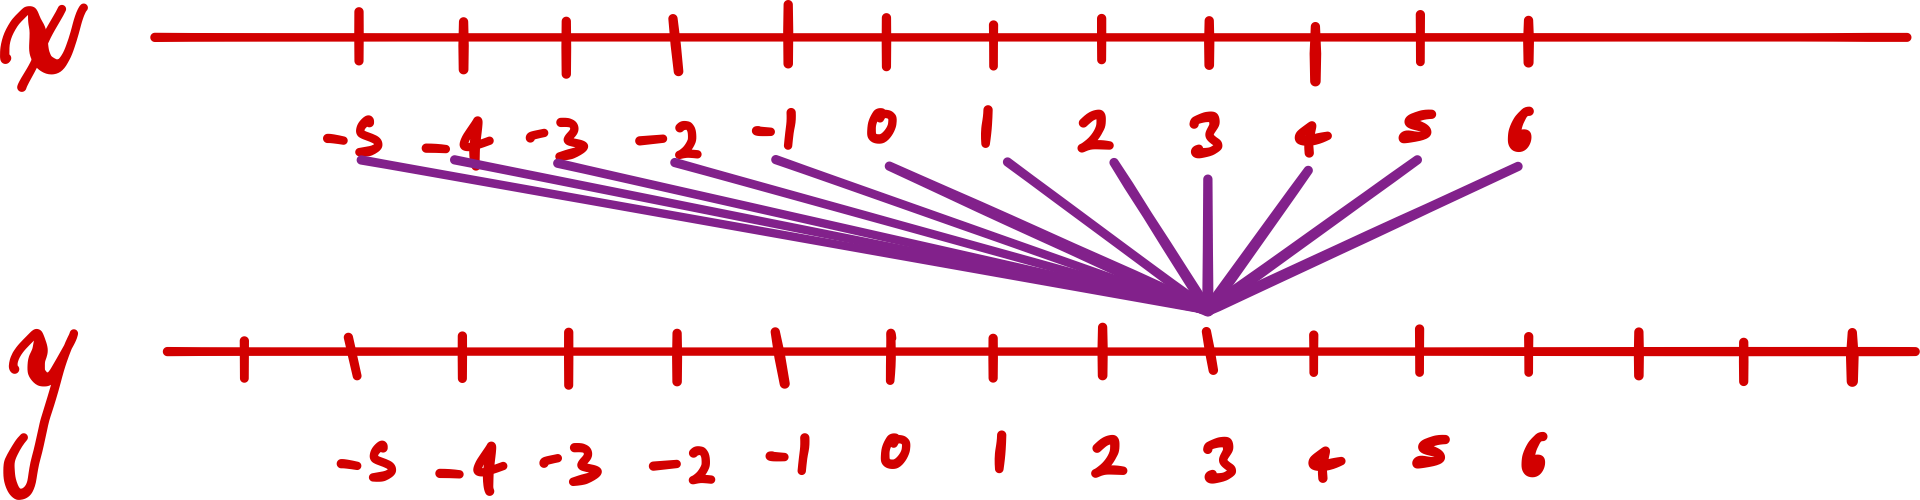
\includegraphics[width=0.7\linewidth]{"./media/ComplexFunctions/PNG image.png"}
	\caption{}
	\label{fig:png-image}
\end{figure}

A similar constant complex function would be $f\left( z \right) =  3 +  4i$:
\begin{figure}[h!]
	\centering
	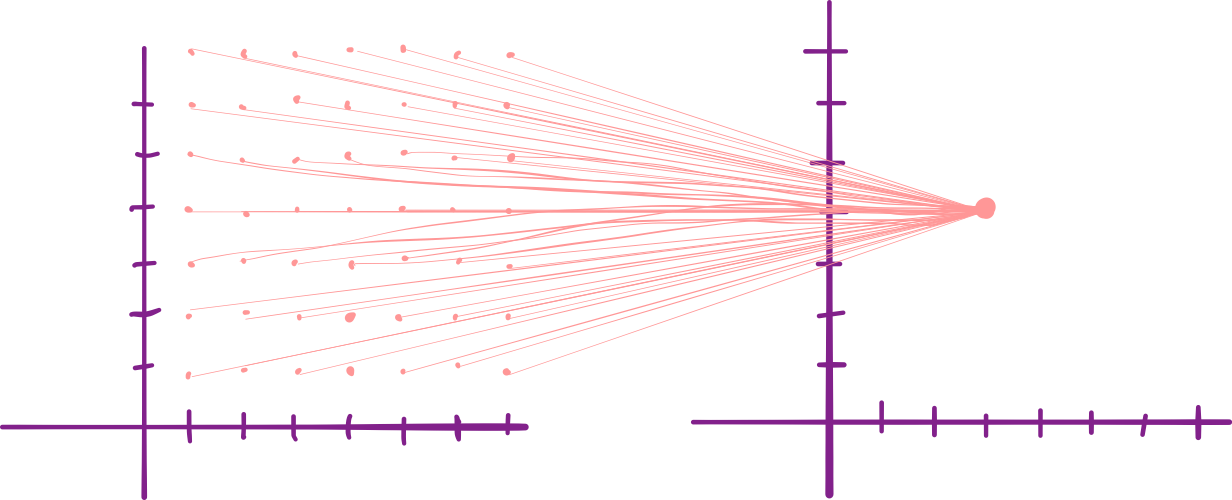
\includegraphics[width=0.7\linewidth]{"./media/ComplexFunctions/PNG image 2.png"}
	\caption{}
	\label{fig:png-image-2}
\end{figure}

It isn't possible to make a graph like it is with simple single variable real functions because that would require four spacial dimensions in order to plot it, this has the dissapointing consequence that geometric interpretations of derivatives as a slope and integrals as area beneath a curve are no longer helpful. \\

It isn't uncommon to use a 3D Cartesian plane to illustrate a function from the reals onto the complex, e.g. imagine $ y =  x^{2}$, if a complex domain is ullustrated as an $x$ /$y$ plane and a perpendicular $z$-axis represents the real codomain, the surface representing the values would always have two roots, even if the're not real, the \textit{Welch Labs} video \textit{Imaginary Numbers are real}\footnote{https://www.youtube.com/watch?v=T647CGsuOVU} is really good for getting a visualisation of this but the general visualisation is:


\begin{figure}[h!]
	\centering
	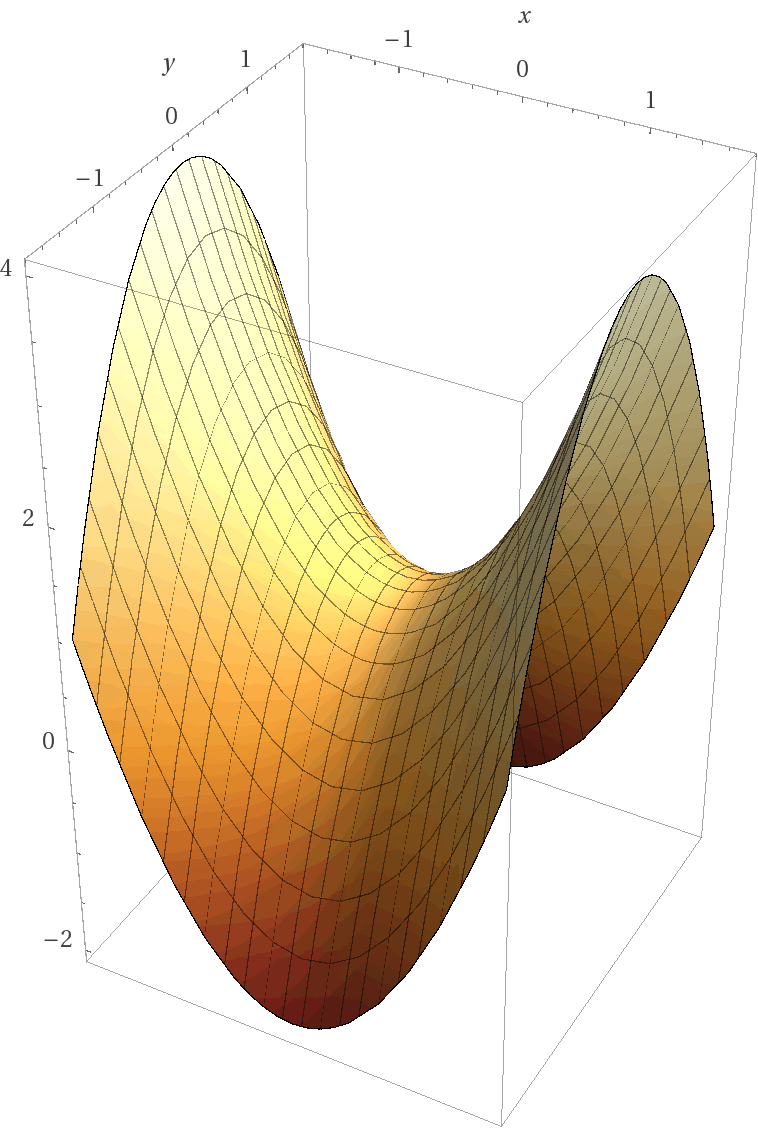
\includegraphics[width=0.2\linewidth]{"./media/ComplexFunctions/PNG image 3.png"}
        \caption{This can be generated in \textit{Wolfram} or something else by using $f(x,y) = \left( x +  i y \right)^2 +  1$}
	\label{fig:png-image-3}
\end{figure}


\section{Complex functions Components}
Complex functions can be illustrated as a pair of two-variable real functions.
Take a function:
\[
  f\left( z \right) =  w
\]
The $w$ variable can be expanded:

\[
  f\left( z \right) =  u +  iv
\]
the $z$ variable can also be expanded:
\[
  f\left( x +  i y  \right) =  u +  iv
\]
Observe that the value $ u$ is in essence a function of the $x$ and $y$ input variables, the same is true also for $v$,  hence, this can be rewritten:

\[
  f\left( x +  i y \right) =  u \left( x,y \right) +  i \times v\left( x,y \right)
  \]

\paragraph{Example}
\begin{align*}
  f\left( z \right) &= z^2 \\
  &= \left( x +  iy  \right)^{2} \\
  &=  x^2 - y^2 +  i \cdot 2xy \\
  &=  \left( x^2 - y^2  \right) +  i \cdot \left( 2xy \right)
  \intertext{So in this case the component functions would be:}
  u\left( x,y \right) &=  \left( x^2 -  y^2 \right) &&\text{and,}\\
  v\left( x,y \right) &=  \left( 2xy \right)
\end{align*}

Essentially a complex-valued function is a pair of two variable real functions.
\subsection{Limits}
if $f$ is defined on all poiints in a \textit{deleted neighbourhood} of $\alpha$ it is written:
\[
  \lim_{z \rightarrow \alpha}{f\left( z \right) = L}, \qquad \text{equivalently,} \qquad f\left( z \right) \rightarrow w_0 \text{\quad as \quad} z \rightarrow z_0.
\]
if and only if:


\hfill\begin{minipage}{\dimexpr\textwidth-3cm}
  $f\left( z \right)$ can be made arbitrarily close to $L$ by making $z$ sufficiently close to $\alpha$.
\end{minipage}
\\ \

In formal notation this is expressed:\\

\ \
\hfill\begin{minipage}{\dimexpr\textwidth-3cm}
\begin{tcolorbox}

  \subparagraph{Formal Definition of a Complex Limit}  \ \\
  \ \\
  If $f: A \rightarrow \mathbb{C} $ and $\alpha \in \overline{A}$ 
\begin{align*}
    \forall \varepsilon > 0, \enspace \exists \delta:& \\
    & 0 <     \left| z-\alpha \right| < \delta \implies     \left| f\left( z \right) - L \right| < \varepsilon
\end{align*}
\end{tcolorbox}

\end{minipage}
\\ \

\newpage 

\paragraph{Limits in Terms of Sequences}
A sequence of complex numbers $\left\{ z_n \right\}_{1}^{\infty}$ has a limit $z$ ( i.e. it converges to $z$) if:\\



\hfill\begin{minipage}{\dimexpr\textwidth-3cm}
\begin{tcolorbox}

  \subparagraph{Formal Definintion of a Limit to a Complex Sequence}
\begin{align*}
    \forall \varepsilon > 0, \enspace \exists N \in \mathbb{Z} :& \\
    i& n > N \implies     \left| z_n - z \right| < \varepsilon
\end{align*}
\end{tcolorbox}

\end{minipage}
\ \\

So this says, the limit of the sequence is $z$ iif the terms of the sequence can be made arbitrarily close to the limit value by moving sufficiently far along the sequence.\\


Limit values are unique, a function can only have a single limite value at a point (or no limit value if the limit is undefined at that point). \\


\paragraph{Limits from multiple directions}\ \\
A single variable real functions can only approach a variable from the left-hand side or the right-hand side, complex funcitons however can approach a varible along any curve in the complex plane. \\

So for example consider the limit of a function as  $z     \rightarrow 0$, $z$ could approach zero along:

\begin{itemize}
  \item the real-axis $\left( x, 0 \right) : x     \rightarrow 0 \implies z     \rightarrow 0$ 
  \item the imaginary-axis $\left( 0, y \right) : y     \rightarrow 0 \implies z     \rightarrow  0$
  \item any straight-line $y = mx : y     \rightarrow 0 \implies z     \rightarrow 0$
  \item along a parabola $y = x^2 : y     \rightarrow 0 \implies z     \rightarrow 0$
  \item any curve whatsoever at all\dots
\end{itemize}

What makes this more confusing is that a limit may approach a value along one curve but not another, maybe for example our function approaches $w = f \left( z \right) = L$ as the variable approaches 0 on both the  $x$-axis and the $y$-axis, despite this it's entirely possible that our function approaches the value 33 along a parabola, the value 42 along a straight line and maybe $6 \pi +  4i$ along a cubic curve. \\


So it's really worth noting that as a \textbf{necessary but not sufficient condition}, the limit taken along the axis must be equal in order for the limit to exist, if they are equal however, the limit is not guaranteed to exist, it may be another value along a different curve. It's worth reading \textit{Pauls Online Notes} \footnote{http://tutorial.math.lamar.edu/Classes/CalcIII/Limits.aspx}\\

The reason for often taking limits along the axis (as opposed to some other arbitrary curve), is because  the axis zeroes out a term which can be simpler and because the partial derivatives are also taken along the axis, which is used in developing the \textit{Cauchy Riemann} equations later, but, really, there is no difference taking the limit along arbitrary curves or along the axis, the function doesn't necessarily care. \\

\newpage 

\paragraph{Theorems on Limits}
The idea here is to establishh a connection between limits of complex functions and limits of real functions so we can use all the pre-established properties of real limits from calculus. \\


if:
\begin{align*}
z &=  x +  i y \\
f\left( z \right) &=  u\left( x, y \right) +  i \cdot  v \left( x, y  \right)
\end{align*}

Then we have:
\[
  \lim_{z \rightarrow \alpha} \left( f\left( z \right) \right) =  L
\]
if and only if:

\[
  \lim_{\left( x, y \right)     \rightarrow \left( a, b \right) }\left[ u \left( x, y \right)  \right] = \operatorname{Re}\left( L \right) \quad \text{and} \quad \lim_{\left( x, y \right)     \rightarrow \left( a,b \right) }\left[ v\left( x,y \right)  \right] = \operatorname{Im}\left( L \right) 
\]

So now we can break the complex limits up into real components that we already know how to deal with, and all the familiar \textit{Limit Laws} carry over from earlier calculus.

\paragraph{Limit Laws}

\subparagraph{Distribution over Addition}
\[
\lim_{z     \rightarrow z_0}\left[ f \left( z \right) g \left( z \right)  \right] =  \lim_{z     \rightarrow z_0}\left[ f \left( z \right)  \right] + \lim_{z     \rightarrow z_0}\left[ g \left( z \right)  \right] 
\]
\subparagraph{Distribution over Multiplication}
\[
\lim_{z     \rightarrow  z_0}\left[ f \left( z \right) \cdot g \left( z \right)  \right] = \lim_{z     \rightarrow  z_0}\left[ f \left( z \right)  \right] \cdot \lim_{z     \rightarrow  z_0}\left[ g \left( z \right)  \right] 
\]
\subparagraph{Distribution over Division}\ \\
Assume that $\lim_{z     \rightarrow  z_0}\left[ g \left( z \right)  \right] \neq 0$:
\[
  \lim_{z     \rightarrow  z_0}\left[ \frac{f \left( z \right) }{g \left( z \right) } \right] = \frac{\lim_{z     \rightarrow  z_0}\left[ f \left( z \right)  \right] }{\lim_{z     \rightarrow  z_0}\left[ g \left( z \right)  \right] }
\]



\paragraph{Riemann Sphere}
Limits at infinity are given a theoretical foundation using an idea called the \textit{Riemann Sphere}, it's interesting but a deep understanding of the theory isn't necessary in order to work with limits at infinity so dont worry about it.

\newpage

\section{Continuity}
A function $f$ is  \textit{continuous} at a point $z_0$ if for all points $\lim_{z     \rightarrow z_0}\left[ f \left( z \right)  \right] = f \left( z_0 \right) $.

This is generally broken up into three conditions for want of decomposing problems:\\


\hfill\begin{minipage}{\dimexpr\textwidth-3cm}
\begin{tcolorbox}

  \subparagraph{Conditions of Continuity}\ \\
  A function $f$ is \textit{Continuous} at $z_0$ if the following three conditions are all satisfied:
  \ \\
  \begin{enumerate}
    \item $\lim_{z     \rightarrow  z_0}\left[ f \left( z \right)  \right] $ \\
    \item $f \left( z_0 \right) $ exists \\
    \item $\lim_{z     \rightarrow   z_0}\left[ f \left( z \right)  \right] = f \left( z_0 \right) $ {\tiny (which implies the above 2)}
  \end{enumerate}
\end{tcolorbox}

\end{minipage}
\ \\




If a function is continuous on some neighbourhood, it's limit value for any point in that neighbourhood is the function value, this means, if we did, for instance, take the limit at a point along both axis (or along any two arbitrary curves), and they were equal, then the limit would be defined at that point, because it would be the function value.\\

If a function can be differentiated at a point, the function is continuous at that point. \\

So if we could show that a derivative exists on all points of some neighbourhood, and that the derivative was continuous at some point, then that neighbourhood would be continuous and the limit at that point would certainly exist. \\

\hfill\begin{minipage}{\dimexpr\textwidth-3cm}
This might seem a little bit contrived, but these are the pieces that are used for the \textit{Cauchy Riemann} equations 
\end{minipage}
\ \


\newpage


\paragraph{Function Composition}\ \\
A composition of continuous functions is continuous, e.g. \ \\
\ \\
if:
\begin{align*}
  f \left( x \right) &= x^2 \quad &\text{is continuous} \\
  g \left( x \right) &= e^x \quad &\text{is contninous}
\end{align*}
Then:
\begin{align*}
  f \circ g =  f \left[  g \left( x \right)  \right]  &=  e^{x^{2}} &\text{is continuous}
\end{align*}
\ \\
Again, this might seem obvious, but it's useful for complex functions and is necessary in the \textit{Cauchy Riemann} equations.


\subparagraph{Continuity of Complex Functions}
A Complex function is only continuous if the real two-variable components $u \left( x, y \right)$ and $v \left( x,y \right) $ are continuous:\\

\hfill\begin{minipage}{\dimexpr\textwidth-3cm}
  {\footnotesize This is because a composition of continuous functions is continuous}
\end{minipage}
\ \\

\begin{figure}[h!]
	\centering
	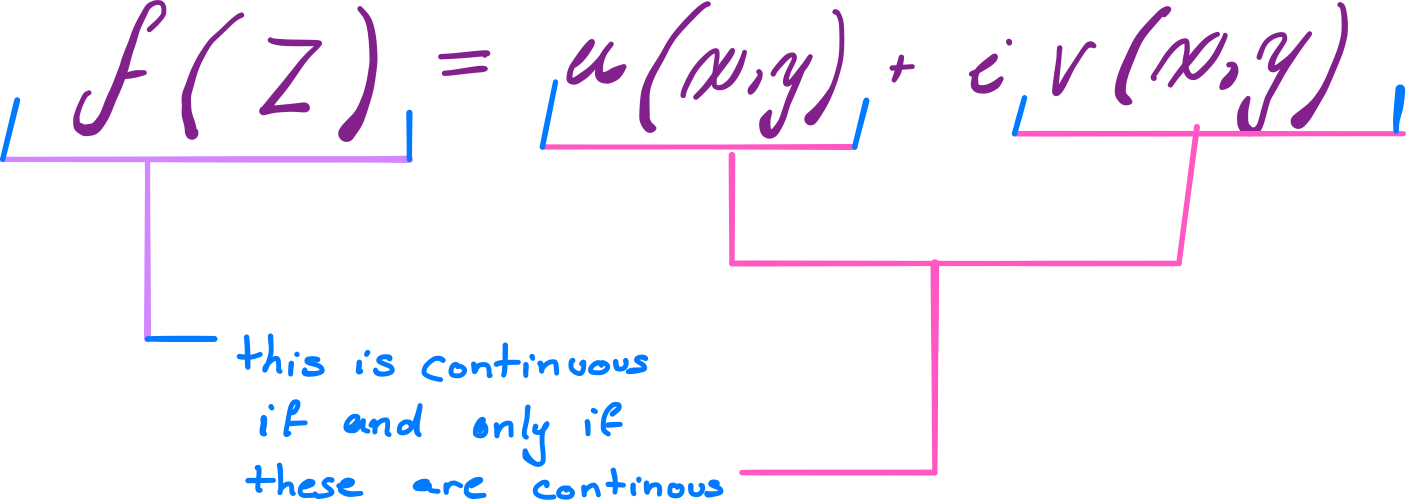
\includegraphics[width=0.7\linewidth]{"./media/ComplexFunctions/PNG image 4.png"}
%	\caption{}
	\label{fig:png-image-4}
\end{figure}

Again, remember this for later when we are doing the \textit{Cauchy Riemann} equations.


\newpage


\section{Derivatives}
Derivatives have the same definition in complex analysis as they do in real calculus, with the difference that the variable is now complex, the derivative of $f$ at $a$ is:

  \begin{align*}
    w &= f \left( z \right)\\
    &\implies \frac{\operatorname{d} w}{\operatorname{d} z} = \lim_{\Delta Z\rightarrow 0}\left[ \frac{\Delta w}{\Delta z} \right] 
  \end{align*}

Or in a more useful fashion:

\[
  f'\left( a \right) = \lim_{\Delta Z\rightarrow 0}\left[ \frac{f \left( z \right) - f \left( a \right) }{z - a} \right] = \lim_{\Delta Z\rightarrow 0}\left[ \frac{f \left( a + \Delta z \right) -  f \left( a \right) }{\Delta z} \right] 
\]

A function may be differentiable at a point $z$ but not necessarily at any other points in the neighbourhood of $z$. \\

The real and imaginary components of a function may have continuous partial derivatives (of all orders) yet this does not imply that the function is differentiable there, 

\ \

\hfill\begin{minipage}{\dimexpr\textwidth-3cm}
e.g.  $   f\left( z \right) =   \left| z \right|$ has continuous partial derivatives away from $z =  0$, but is not differentiable anywhere, because the limits as $\Delta   z  \rightarrow 0$ are different depending on which path is taken.\end{minipage}
\ \





\paragraph{Conditions of Continuity}
\begin{itemize}
  \item if a function is continuous it may or may not be differentiable
  \subitem continuity $ \centernot\implies $ differentiability
  \item if a function is differentiable it must be continuous
  \subitem differentiability $ \implies  $ continuity
\end{itemize}

\subsection{Derivatives to Memorise}
The following complex functions are nowhere differentiable:

\begin{itemize}
  \item $f\left( z \right)  = \Re{\left( z \right) }$ 
  \item $f\left( z \right) = \Im{\left( z \right) }  $ 
  \item $f\left( z \right)  = \overline{z}$ 
\end{itemize}

The function $f\left( z \right) =      \left| z \right|^{2}$ is differentiable only at $z =  0$:
\[
  \frac{\operatorname{d} }{\operatorname{d} z}\left(     \left| z \right|^{2} \right) \Big|_{z =  0} = f'\left( 0 \right) = 0
\]

bear in mind however that this function is nowhere analytic, because it is not differentiable on a neighbourhood of 0, this is covered further down.

\paragraph{How to Deal with Derivatives}
If you are given a function purely of $z$, then all the familiar differentiation rules carry over, their proofs are different, but the rules come out the same.  
\footnote{I mean, be careful with $\log$ functions and roots because they have multiple values}\\

If however you are given a function with terms of $z$, $x$ and $y$, then you will need to first break the function up into it's components:

\[
  f\left( z \right)  =  u\left( x,y \right) + i\cdot v\left( x,y \right) 
\]

and then you will need to use the \textit{Cauchy Riemann} equations, which we will get to further down.

\paragraph{Example}
Find the derivative of $w =  f\left( z \right) =  \frac{1}{z}$:

\end{document}

 %\input{08_vars/drawing.tex}
 %
 \chapter{Complex Functions}
 %\documentclass[article]{standalone}
\documentclass[class=article, crop=false]{standalone}

\usepackage{./resources/style}
\usepackage{./resources/referencing}


 \title{(09) Elementary Functions}
\date{Analysis (200023)}
\author{Analysis (200023)}

\begin{document}
%	\maketitle
%	\tableofcontents

\section{Polynomial Functions}
    an $n^{\mathrm{th}}$ degree polynomial is given by:

    \[
      p\left( z \right)  =  w =  \alpha_0 +  \alpha_1z_1+  z_2 \dots \alpha_nz_n
    \]
        where:
    \begin{itemize}
      \item $\alpha$ is a complex constant
      \item $z$ is a complex variable
    \end{itemize}

    \section{Rational Function}
    A rational function is composed of two polynomial functions $P\left( z \right) $ and $Q\left( z \right) \neq 0$ :
    \[
      \frac{P\left( z \right) }{Q\left( z \right) }
    \]


\newpage


    \section{Euler's Formula}
    This is really important, and there are lots of proofs for it, for the most part though, just come to accept it, the best justification for \textit{Euler's Formula} that I've seen is by \href{https://www.youtube.com/watch?v=mvmuCPvRoWQ}{\textit{3Blue1Brown}}, Seriously, watch this, it's really good.

    \begin{align*}
      e^{i\theta} &=  \cos{\theta} +  i \cdot  \sin{\theta} \\
      \implies   r \cdot e^{i\theta} &= r \left( \cos{\theta} +  i \cdot  \sin{\theta} \right) \\
      r \cdot  e^{i\theta} &=  r \cdot  \mathrm{cis}{\left( \theta \right) } \\
      &= z
    \end{align*}

    It is not uncommon to see Euler's formula used instead of polar notation, particularly in the \textit{Churchill} text, don't stress out, it has the same meaning in effect.

    \section{Exponential Function}
    The exponential function is defined for all complex values:
    \begin{align*}
      e^z =  e^{x +  iy} &= e^x \cdot e^iy \\
      &= e^x \cdot  \left(  \cos{y} +  i \cdot  \cos{y} \right)
    \end{align*}
    \subsection{Modulus and Argument}
    because:
    \[
    e^z = e^x\cdot \mathrm{cis}{\left( y \right) }
    \]
\noindent    we have the modulus:
    \[
            \left| e^z \right| = e^x
    \]

\noindent and the argument:
    \[
        \operatorname{arg}\left( e^z \right) = y + 2\pi k \qquad \left( k \in \mathbb{Z}^*  \right)
    \]\\

    \hfill\begin{minipage}{\dimexpr\textwidth-3cm}
      the notation $\mathbb{Z}^* $ means 'non-negative integers' so, $\left( 0, 1, 2, 3 \dots \right) $
    \end{minipage}
    \ \




    \section{Properties of the exponential function}
    \paragraph{Periodicity}
    The complex exponential function is periodic:
    \[
      e^{z +  2\pi i} =  e^z
    \]
    This corresponds the sliding action of $z +  2 \pi i$ to a rotation of $x +  2 \pi$ radians of rotation, because the rotation has a period of $2 \pi$, the rotation will be $x$ radians.

    For this reason we also have:
    \begin{align*}
    e^z &=  e^z\\
    \left( e^z \right)^{\frac{1}{n}}  &=  e^{\frac{z +  2 k \pi}{n}}
    \end{align*}

    \paragraph{Principle Argument}
    We choose the principle argument as $(-\pi, \pi]$, this is useful later on for dealing with logs.
    \begin{itemize}
      \item The Principle Argument of a complex function is denoted by a capital:
        \subitem $\operatorname{Arg}\left( r \cdot \mathrm{cis}{\theta} \right) = \theta$
      \item The general Argument of a complex function is denoted by lower case:
        \subitem $\operatorname{arg}\left( r\cdot \mathrm{cis}{\left( \theta \right) } \right) = \theta +  2\pi k \qquad :\enspace k \in \mathbb{Z}^+$
    \end{itemize}

    \paragraph{Differentiating $e^z$}
    So if you want to just move on:
    \[
    \frac{\operatorname{d} }{\operatorname{d} z}\left[ e^z \right] = e^z
    \]
    If you want to know why:

    \begin{align*}
      \frac{\operatorname{d} }{\operatorname{d} z}\left( e^z \right) &= \frac{\partial }{\partial x} \left[ e^{x +  iy} \right] +  i \cdot \frac{\partial }{\partial y}\left[ e^{x + iy} \right] \\
      &= \frac{\partial }{\partial x}\left[ e^x \cos{y} \right] + \frac{\partial }{\partial x}\left[ e^x \sin{y} \right] \\
      &= \cos{y}e^x +  \sin{y}e^x\\
      &= e^{x + iy}\\
      &= e^z
    \end{align*}
    \begin{flushright}
    {\rule{0.7em}{0.7em}}
    \end{flushright}

    \paragraph{Polar Form}
    The exponential function can be expressed as:
    \begin{align*}
    e^z &= e^x \cdot \left( \cos{y} +  i \sin{y} \right) \\
    &= e^x\cdot \mathrm{cis}{y}
    \end{align*}


    \begin{alignat*}{5}
    & \implies  &\operatorname{Arg}\left( e^z \right)& &= &y\\
    & \implies  &\operatorname{arg}\left( e^z \right)& &= &y + 2\pi\\
    &  \implies      &\left| e^z \right|& &= &e^x
    \end{alignat*}

    \paragraph{Additional Properties}
    Consider that $\forall x,y \in \mathbb{R} $ $e^x \neq 0$ and also that $e^{iy} \neq 0$, hence:
    \[
      e^{z} = e^x \cdot e^{iy} \neq 0
    \]

    Although many things carry over, be careful because:
    \[
      e^x \nleq 0 \qquad \text{   however   } \qquad e^z < 0 \quad \vee  \quad  e^z > 0
    \]

\newpage

    \section{The Log Function}


    \subsection{Deriving the Log Function}
    With real variables the motivation for the log function is a function for $y$ such that:
    \[
    e^y = x
    \]
    In the complex case the motivation is much the same:
    \[
    e^w =  z
    \]
    So in order to solve a value for the complex logarithm express $z$ in polar form and decompose $w$ into a real and complex part:

   \begin{align*}
   e^w =  z  \implies   e^{u +  iv} &=  r e^{i\theta}\\
   	e^u \cdot  e^{iv} &=  re^{i\theta}
  	\end{align*}

        Equate the real and imaginary parts

\begin{multicols}{2}
  \begin{align*}
    e^u &= r\\
     \implies  u &= \ln{\left( r \right) }
  \end{align*}\break
  \begin{align*}
      e^{iv} &= e^{i\theta}\\
      \implies  v &=  \theta +  2\pi k, \qquad k \in \mathbb{Z}^+
  \end{align*}
\end{multicols}

so the equation $e^w= z$ is satisfied if and only if:
\begin{align*}
  w &=   u +  iv\\
  &=  \ln{\left( r \right) } +  i \cdot  \left(  \theta +  2\pi k \right) , \qquad k \in \mathbb{Z}^+\\
    &= \ln{\left|      z   \right| } +  i \cdot \operatorname{arg}\left( z \right)
\end{align*}


\ \

\ \

\hfill\begin{minipage}{\dimexpr\textwidth-3cm}
\begin{tcolorbox}

  \subparagraph{Complex Logarithm}
  A value in the complex plane $z= r\cdot e^{i\cdot \theta}=  r\cdot \mathrm{cis}{\left( \theta \right) } \in \mathbb{C} $ will have a logarithm:
\begin{align}
  \log_e{\left( z \right) } = \ln{     \left| z \right| + i\cdot \operatorname{arg}\left( z \right)  } \label{compdef}
\end{align}
\end{tcolorbox}

\end{minipage}
\ \\

The Complex Logarithm isn't a function, it is what is known in complex analysis as a '\textit{multiple-valued function}' which is merely a \href{https://en.wikipedia.org/wiki/Multivalued_function}{\textit{binary relation}} \footnote{\url{https://en.wikipedia.org/wiki/Multivalued_function}}, this is really ambiguous though because clearly a function can only have one output, the terminology is used to respect the fact that if, for example, $\log_e{\left( z \right) }$, is restricted to a single branch, it is indeed a function.
\ \\



\newpage



\subsection{Notation}



    \paragraph{Base}\ \\
    Also another really confusing point is that often times in complex analysis $\operatorname{log}\left( z \right)$ is used to represent the complex natural logarithm and $\ln{\left( x \right) }$ is used to represent the real natural logarithm, so you might see $\operatorname{log}$ and immediately think base-10, but don't, we deal excusively in $e$ with complex awnalysis.\\

    It's all redundant anyway because the change of base formula applies also to complex logarithm's anyway.\\

    For clarity sake, I'll write $\log_e{\left(  \right) }$ when dealing with complex natural logarithms and $\ln{\left(  \right) }$ when dealing with real natural logarithms.

    \subsection{Change of Base}
    So in this example our desired solution is $y$ :

    \begin{align*}
      10^y &= e +  4i\\
      \mathrm{Log}_e{\left( 10^y \right) } &=  \mathrm{Log}_e{\left( 3 +  4i \right) } \\
      y \cdot  \mathrm{Log}_e{\left( 10 \right) }&= \mathrm{Log}_e{\left( 3 +  4i \right) }\\
      y &=  \frac{\mathrm{Log}_e{\left( 3 +  4i \right) }}{\mathrm{Log}_e{\left( 10 \right) }} \\
&\implies      \mathrm{Log}_{10}{\left( 3 + 4i \right) } =  \frac{\mathrm{Log}_e{\left( 3 +  4i \right) }}{\mathrm{Log}_e{\left( 10 \right) }}
    \end{align*}
    \begin{flushright}
    {\rule{0.7em}{0.7em}}
    \end{flushright}


    This works because $\mathrm{Log}_e{\left(  \right) }$ is a valid function, it should work with other branches but I'm not sure.


\newpage



\paragraph{Arguments}\ \\
%The exponential function is periodic, so, it stands to reason that there will be multiple solutions for the logarithmic function.\\
The principal argument corresponds to $\theta \in (-\pi,\pi]$ and is distinguished by using uppercase:
    \begin{itemize}
      \item Principal Argument:
\subitem        $\operatorname{Arg}\left( z \right) = \Theta \qquad -\pi < \Theta \leq \pi$
\subsubitem So less that or equal to $\pi$ but $\Theta \neq \pi$
\item Argument:
  \subitem $\operatorname{arg}\left( z \right) = \theta =  \Theta + 2\pi k  \qquad \left( k \in \mathbb{Z}  \right) $
  \subsubitem This is periodic.
    \end{itemize}
    So for example, we may have $r \cdot \mathrm{cis}{\left( \theta \right) } =  r\cdot \mathrm{cis}{\left( \Theta \right) }$ the difference being that
    \begin{itemize}
      \item $\theta \in \mathbb{R} $
      \item $\Theta \in (-\pi, \pi]$
    \end{itemize}

    \paragraph{Logarithms}
    \ \

    \hfill\begin{minipage}{\dimexpr\textwidth-3cm}
    \begin{tcolorbox}

    \paragraph{Notation}\ \\
    Where $z =  r \cdot \mathrm{cis}{\left( \theta \right) }$:\\
    \ \\
    The \textbf{Principal Value} of the $\log_e{\left(  \right) }$ function is given by:
    \begin{align}
      \mathrm{Log}_e{\left( z \right) } &= \ln{     \left| z \right|  } +  i \cdot  \operatorname{Arg}\left( z \right) \\
      &= \ln{ \left( r \right)  } +  i \cdot \Theta
      \label{prinlogdef}
    \end{align}

    The \textbf{multi-valued} log function is given by:

    \begin{align}
      \log_e{\left( z \right) } &= \ln{     \left| z \right|  } +  i \cdot \operatorname{arg}\left( z \right) \\
      &= \ln{ \left( r \right)  } +  i \cdot \left( \Theta + 2\pi k \right) \qquad k \in \mathbb{Z}
      \label{mvlogfunc}
    \end{align}
   \end{tcolorbox}

    \end{minipage}
    \ \\


    \newpage



      \subsection{Branches}
      A branch of a function $f\left( z \right) $ that has multiple outputs  (e.g. $\log_e{\left( z \right) }$), is a function with a single output that is analytic in the domain. \\
At every point of the domain, the single-valued function must assume exactly one of the various possible values that the original function might have given as output.\\
\ \


\hfill\begin{minipage}{\dimexpr\textwidth-3cm}
  The requirement of analyticity prevents $F\left( z \right) $ from taking on a random selection of the values of $f\left( z \right) $.\\
  So in the case of logs:\\
\end{minipage}

\ \

\hfill\begin{minipage}{\dimexpr\textwidth-3cm}
\begin{tcolorbox}

  \subparagraph{Logarithmic Branches}\ \\

  The \textbf{Principal Branch} of the logarithmic function is given by:
  \begin{align}
   \mathrm{Log}_e{\left( z \right) } &= \ln{ \left( r \right)  } +  i \cdot \Phi \qquad -\pi < \Phi < \pi
    \label{pblog}
  \end{align}
  Any \textbf{Branch} of the logarithmic function is given by:
  \begin{align}
    \log_e{\left( z \right) } &= \ln{ \left( r \right)  } +  i \cdot \phi \qquad -\alpha < \phi <\alpha + 2 \pi k
    \label{branchlogdef}
  \end{align}
\end{tcolorbox}

\end{minipage}
\ \\

 here, the \textbf{Principal Value} of the complex log and the \textbf{Principal Branch} are denoted ambiguously by $\mathrm{Log}_e{\left(  \right) }$ but they are both different, for example $\mathrm{Log}_e{\left( -10 \right) }= \ln{ 10 } +  \pi\cdot i$ as the principal value, however, it is entirely undefined on the principal branch.\\

 So basically, on the principal branch, we delete the entire non-positive $x$-axis (i.e. including zero), where as the principal value is allowed to take values there using $\pi$ (but not $-\pi$).\\

 Now one might ask 'why on Earth would we do such a confusing and ambiguous thing?'\\
 The reason is because it is the only way to make the $\log_e{\left(  \right) }$ function continuous and hence analytic.:\\
 \ \

 \hfill\begin{minipage}{\dimexpr\textwidth-3cm}
   Clearly we couldn't use the \textit{multi-valued} log functions as in (\ref{mvlogfunc}) because that has multiple outputs for a given input and so it is not a function, hence it clearly is not analytic.\\

   Now why can't we restrict the domain to the principal argument of $\theta \in (-\pi, \pi]$?\\

   \ \

   \hfill\begin{minipage}{\dimexpr\textwidth-3cm}
   A function must be continuous in order to be differentiable and hence analytic, the condition for continuity is:\\
   \[
   \lim_{z     \rightarrow \alpha}\left[ \mathrm{Log}_e{\left( z \right) } \right] = \mathrm{Log}_e{\left( \alpha \right) }
   \]
But if we take a value on the negative $x$-axis:

\begin{align*}
    \lim_{z     \rightarrow -1}\left[ \mathrm{Log}_e{\left( z \right) } \right] &= + \pi \cdot i  \qquad \left( \text{From Above} \right) \\
    \lim_{z     \rightarrow -1}\left[ \mathrm{Log}_e{\left( z \right) } \right] &= -  \pi \cdot i  \qquad \left( \text{From Below} \right)
\end{align*}

This implies that the limit does not exist, similarly it can be shown that the limit does not exist as $z$ approaches values on the non-posiitive $x$-axis, no limit means no continuity, which  means no differentiablility, which means not analytic.\\

The solution here is to remove the negative $x$-axis and zero from the domain, then the $\mathrm{Log}_e{\left(  \right) }$ function will be analytic.j
\ \\





   \end{minipage}
   \ \


 \end{minipage}
 \ \



\newpage



\paragraph{Branch Cuts}
A branch cut is a curve that is introduced in order to define the multiply defined function $F\left( z \right) $, it's basically the line we have to delete.\\

So imagine $\log_e{\left( z \right) }$:
\ \

\ \
% \begin{figure}[h!]
%
% 	\includegraphics[width=0.4\linewidth]{}
% 	\caption{Polar Representation of $z\in \mathbb{C}$}
% 	\label{fig:handwriting}
% \end{figure}

The principal branch deletes the negative $x$-axis and $0$ as shown in blue below:

% \begin{figure}[h!]
% 	\includegraphics[width=0.4\linewidth]{"handwriting2"}
% 	\caption{Principal Branch Cut}
% 	\label{fig:handwriting-2}
% \end{figure}

\newpage


So for the Complex Logarithm that we used as a definition at (\ref{branchlogdef}), the angle $\alpha$ from the origin is used as the branch cut in order to define a branch.

\ \

\hfill\begin{minipage}{\dimexpr\textwidth-3cm}
  So for example, as above in Figure \ref{fig:handwriting-2}, the line drawn from $0$ at $-\pi$ radians corresponds to $\alpha = - \pi$ in the definition; This line is a branch cut of $\log_e{\left( z \right) }$ that we use to define the principal branch of the logarithmic function:
  \[
  \log_e{\left( z \right) } = \ln{ \left( r \right)  }+ i\cdot \Phi \qquad -\pi < \Phi < \pi
  \]
\end{minipage}
\ \\

Basically you just delete that line in the definition of the domain.\\

Also be aware that the branch cut doesn't have to be a line, it could be a curve, this diagram is an example of a branch cut that would define a valid branch of the $\log_e{\left( z \right) }$ function:

% \begin{figure}[h!]
% 	\includegraphics[width=0.4\linewidth]{"handwriting3"}
% 	\caption{}
% 	\label{fig:handwriting-3}
% \end{figure}

It works because however far the value of $z$ is from the origin, the values of $\theta$ will still be restricted to one revolution.

\subsection{Principal Branch as opposed to Principal Value}
Be aware that there is a difference between the \textit{principal value} and the \textit{principal branch} of the complex natural logarithm:
\begin{itemize}
  \item The \textbf{Principal Value} of the complex logarithmic function of $z = r\cdot \mathrm{cis}{\left( \theta \right) }$ is:
    \subitem $\log_e{\left( z \right) } = \ln{ \left( r \right)  }+ i \cdot \Theta \qquad \Theta \in  (-\pi, \pi]$
  \item The \textbf{Principal Branch} of the complex logarithmic function of $z = r\cdot \mathrm{cis}{\left( \theta \right) }$ is:
    \subitem $\log_e{\left( z \right) } =  \ln{ \left( r \right)  +  i \cdot \Phi \qquad -\pi < \Phi < \pi }$
\end{itemize}

So to be clear, the principal value of $\mathrm{Log}_e{\left( -1 \right) } = \pi i$, however this is entirely undefined on the principal branch.



\newpage

    \subsection{Properties of Complex Logs}
    Familiar properties of logartithms in calculus are sometimes but not aways true in complex analysis, the problem is usually the multiple branches of the log function.

    So one of the first things to be careful with is:
    \[
      e^{\log_e{\left( z \right) }} = z \qquad \text{by definition}
    \]
    However:

    \[
    \log_e{\left( e^z \right) } =  x +  i \cdot \left( y +  2\pi k \right)  \qquad k \in \mathbb{Z}^+ \\
    \]
    But if we take the principal branch:
      \begin{align*}
        \mathrm{Log}_e{\left( e^z \right) } &=  x +  i \cdot  y  \\
        &= e^z
      \end{align*}

      Another one to be careful of, for example:
      \[
        \log_e{\left( i^2 \right) }\neq \frac{1}{2} \cdot \log_e{\left( i \right) }
      \]
      because:
      \begin{multicols}{2}
        \begin{align*}
         \log_e{\left( i^2 \right) } =  \log_e{\left(  - 1 \right) } &= \ln{      \left|  - 1 \right|  } +  i \cdot  \operatorname{arg}\left( - 1 \right) \\
         &=  0 +  \operatorname{arg}\left( - 1 \right) \cdot i\\
         &=  \operatorname{arg}\left( - 1 \right) \cdot i\\
         &= \left( \pi +  2 \pi k \right) \cdot  i\\
         &=  \pi \left(1 +  2k \right) \cdot i
        \end{align*}\break
        \begin{align*}
          2\cdot \log_e{\left( i \right) }&= 2\left[ \ln{     \left| i \right|  }+ \operatorname{arg}\left( i \right) \cdot i \right] \\
          &= 2\left[ o +  \left( \frac{\pi}{2} +  2 \pi k \right) \cdot i \right] \\
          &= i \cdot  \left[  \pi +  4 \pi k \right] \\
          &= \pi\cdot i \left[ 4k+ 1 \right]
        \end{align*}
      \end{multicols}

      If however we choose the principal branch that corresponds to $k =  0$:
      \[
      \log_e{\left( i^2 \right) } = \pi i =  2 \cdot \log_e{\left( i \right) }
      \]



      \newpage

\subsection{Log Laws}
\paragraph{Addition/Multiplication}\ \\
because:
\begin{align*}
\operatorname{arg}\left( z_1 \cdot z_2 \right) &= \operatorname{arg} \left( z_1 \right) +  \operatorname{arg}\left( z_2 \right) \\
\ln{ \left( x_1 \cdot  x_2 \right)  } &=  \ln{ \left( x_1 \right)  }+  \ln{  \left( x_2 \right)  }
\end{align*}
We have:
\ \

\hfill\begin{minipage}{\dimexpr\textwidth-3cm}
\begin{tcolorbox}

Addition of Logs
\begin{align}
  \log_e{\left( z_1 \cdot z_2 \right) }&= \log_e{\left( z_1 \right) } +  \log_e{\left( z_2 \right) }\\
  \log_e{\left( \frac{z_1}{z_2} \right) } &= \log_e{\left( z_1 \right) } -  \log_e{\left( z_2 \right) } \qquad \left( z_2 \neq 0 \right)
\end{align}
\end{tcolorbox}

\end{minipage}
\ \\

Also because:
\[
    \left| z_1 \cdot  z_2 \right|  =      \left| z_1 \right|  \cdot     \left| z_2 \right|
\]
we have:
\[
\log_e{\left(     \left| z_1 \cdot z_2 \right|  \right) } =  \log_e{\left(     \left| z_1 \right|  \right) } +  \log_e{\left(     \left| z_2 \right|  \right) }
\]


\subparagraph{Relationships to Roots}
\begin{align*}
    z^n &=  e^{n\cdot \log_e{\left( z \right) }}\\
    z^\frac{1}{n} &=  e^{\frac{1}{n}\cdot \log_e{\left( z \right) }}\\
    &= e^{\frac{1}{n} \ln{ r } +  \frac{i\left( \theta 2\pi k \right) }{n}}\\
    &= \sqrt[n]{r} \cdot  e^{i \left( \frac{\theta}{n} +  \frac{2k \pi}{n} \right) }\\
      &= \sqrt[n]{r} \cdot \mathrm{cis}{\left( \frac{\theta}{n} +  \frac{2\pi k}{n} \right) }
\end{align*}

\paragraph{Exponentiation}
\begin{align*}
  \log_e{\left( z^n \right) } &=  \ln{      \left| z^n \right|  } +  \operatorname{arg}\left( z^n \right) \\
  &= \ln{ \left(     \left| z \right| ^n \right)  } +  \operatorname{arg}\left( \left[ r\cdot \mathrm{cis}{\theta}^n \right]  \right) \\
  &= n\cdot \ln{     \left| z \right|  } +  \operatorname{arg} \left( rn \cdot \mathrm{cis}{\left( n\theta \right) } \right) \\
  &= n\cdot \ln{     \left| z \right|  } +  \operatorname{arg}\left( \mathrm{cis}{\left( \theta\cdot n \right) } \right) \\
&=   n\cdot \ln{     \left| z \right|  } +  \left( n\theta +  2\pi k \right) \qquad \exists k \in \mathbb{Z}\\
\intertext{This is only valid for a branch of the logarithmic function, in this case choose the principal branch}
  &= n\cdot \ln{     \left| z \right|  }+ n\theta\\
  &= n\cdot \mathrm{Log}_e{\left( z^n \right) }
\end{align*}

Therefore the exponential log law carries over where we use a single branch of the complex logarithmic function.


\newpage

\subsection{Differentiating $\log_e{\left( z \right) }$}

\hfill\begin{minipage}{\dimexpr\textwidth-3cm}
\begin{tcolorbox}
  \paragraph{Derivative of complex log}
\begin{align}
  \frac{\operatorname{d} }{\operatorname{d} z}\left( \mathrm{Log}_e{\left( z \right) } \right) &= \frac{1}{    \left| z \right| \cdot \mathrm{cis}{\left( \operatorname{Arg}\left( z \right)  \right) }} \label{logdiff}
\end{align}
If you're not dealing with the principal branch adjust the argument accordingly, the derivative is only defined for a branch of the logarithmic function.
\end{tcolorbox}

\end{minipage}
\ \\
\ \\
The working for this is pretty straight-forward.
\begin{align*}
  f\left( z \right) = \log_e{\left( z \right) } &= \ln{     \left| z \right|  } +  i \left( \operatorname{arg}\left( z \right) + 2\pi k \right) \\
  \intertext{Let $\theta =  \operatorname{arg}\left( z \right) $}
  &= \ln{     \left| z \right|  } + \left( \theta +  2\pi k \right) \\
  \intertext{Choose a branch of $\log_e{\left( z \right) }$ so that it is a function}
  &= \ln{     \left| z \right| + i\Phi}  \qquad -\alpha < \Phi < \alpha + 2\pi k
  \intertext{let $r =     \left| z \right| $}
  &= \ln{ \left( r \right)  } +  i \Phi\\
\end{align*}
\begin{multicols}{2}
  Let $u =  \ln{ \left( r \right)  }$:
  \begin{flalign*}
      u_r &= \frac{1}{r}&\\
      u_\Phi &= 0
  \end{flalign*}\break
  Let $v =  \Phi $:
  \begin{flalign*}
    v_\Phi &= 1&\\
    v_r &= 0
  \end{flalign*}
\end{multicols}
Our domain is $r>0$, so $\frac{\partial u }{\partial r}$ and $\frac{\partial v }{\partial \Phi}$ are continuous on the entire domain.\\

because $f\left( z \right) =  u\left( r,\Phi\right)  +  i \cdot  v\left( r, \Phi \right) $, use the polar form of the \textit{Cauchy Riemann} equations :
\ \\
\begin{multicols}{2}
  First Condition:
  \begin{flalign*}
    r\cdot u_r &= v_\Phi&\\
    r \cdot \frac{\partial }{\partial r} \cdot \left( \ln{ \left( r \right)  } \right) &= \frac{\partial }{\partial \Phi}\left( \Phi \right) &\\
    r \times \frac{1}{r}&= 1 &\\
    1 &= 1
  \end{flalign*}\break
  Second Condition:
  \begin{flalign*}
      u_\Phi &=  - r\cdot v_r&\\
      \frac{\partial }{\partial \Phi}\left( \ln{ \left( r \right)  } \right) &= - r \times \frac{\partial }{\partial r}\left( \Phi \right) &\\
      0 &=  - r \times 0 &\\
      0 &= 0
  \end{flalign*}
\end{multicols}
both the \textit{Cauchy Riemann} equations are satisfied so:
\begin{align*}
    \frac{\operatorname{d} }{\operatorname{d} z}\left( \log_e{\left( z \right) } \right) = e^{- i\Phi} \cdot \left( u_r + iv_r \right) \\
    &= e^{- i\Phi}\cdot \left( \frac{1}{r} + i \times 0 \right) \\
    &= \frac{1}{re^{i\Phi}}\\
    &= \frac{1}{r\cdot \mathrm{cis}{\left( \Phi \right) }} \\
    &= \frac{1}{    \left| z \right| \cdot \mathrm{cis}{\left( Arg\left( z \right)  \right) }}
\end{align*}
 \ \




\end{document}

 %%\documentclass[article]{standalone}
\documentclass[class=article, crop=false]{standalone}

\usepackage{./resources/style}
\usepackage{./resources/referencing}


 \title{(09) Elementary Functions}
\date{Analysis (200023)}
\author{Analysis (200023)}

\begin{document}
%	\maketitle
%	\tableofcontents

\section{Polynomial Functions}
    an $n^{\mathrm{th}}$ degree polynomial is given by:

    \[
      p\left( z \right)  =  w =  \alpha_0 +  \alpha_1z_1+  z_2 \dots \alpha_nz_n
    \]
        where:
    \begin{itemize}
      \item $\alpha$ is a complex constant
      \item $z$ is a complex variable
    \end{itemize}

    \section{Rational Function}
    A rational function is composed of two polynomial functions $P\left( z \right) $ and $Q\left( z \right) \neq 0$ :
    \[
      \frac{P\left( z \right) }{Q\left( z \right) }
    \]


\newpage


    \section{Euler's Formula}
    This is really important, and there are lots of proofs for it, for the most part though, just come to accept it, the best justification for \textit{Euler's Formula} that I've seen is by \href{https://www.youtube.com/watch?v=mvmuCPvRoWQ}{\textit{3Blue1Brown}}, Seriously, watch this, it's really good.

    \begin{align*}
      e^{i\theta} &=  \cos{\theta} +  i \cdot  \sin{\theta} \\
      \implies   r \cdot e^{i\theta} &= r \left( \cos{\theta} +  i \cdot  \sin{\theta} \right) \\
      r \cdot  e^{i\theta} &=  r \cdot  \mathrm{cis}{\left( \theta \right) } \\
      &= z
    \end{align*}

    It is not uncommon to see Euler's formula used instead of polar notation, particularly in the \textit{Churchill} text, don't stress out, it has the same meaning in effect.

    \section{Exponential Function}
    The exponential function is defined for all complex values:
    \begin{align*}
      e^z =  e^{x +  iy} &= e^x \cdot e^iy \\
      &= e^x \cdot  \left(  \cos{y} +  i \cdot  \cos{y} \right)
    \end{align*}
    \subsection{Modulus and Argument}
    because:
    \[
    e^z = e^x\cdot \mathrm{cis}{\left( y \right) }
    \]
\noindent    we have the modulus:
    \[
            \left| e^z \right| = e^x
    \]

\noindent and the argument:
    \[
        \operatorname{arg}\left( e^z \right) = y + 2\pi k \qquad \left( k \in \mathbb{Z}^*  \right)
    \]\\

    \hfill\begin{minipage}{\dimexpr\textwidth-3cm}
      the notation $\mathbb{Z}^* $ means 'non-negative integers' so, $\left( 0, 1, 2, 3 \dots \right) $
    \end{minipage}
    \ \




    \section{Properties of the exponential function}
    \paragraph{Periodicity}
    The complex exponential function is periodic:
    \[
      e^{z +  2\pi i} =  e^z
    \]
    This corresponds the sliding action of $z +  2 \pi i$ to a rotation of $x +  2 \pi$ radians of rotation, because the rotation has a period of $2 \pi$, the rotation will be $x$ radians.

    For this reason we also have:
    \begin{align*}
    e^z &=  e^z\\
    \left( e^z \right)^{\frac{1}{n}}  &=  e^{\frac{z +  2 k \pi}{n}}
    \end{align*}

    \paragraph{Principle Argument}
    We choose the principle argument as $(-\pi, \pi]$, this is useful later on for dealing with logs.
    \begin{itemize}
      \item The Principle Argument of a complex function is denoted by a capital:
        \subitem $\operatorname{Arg}\left( r \cdot \mathrm{cis}{\theta} \right) = \theta$
      \item The general Argument of a complex function is denoted by lower case:
        \subitem $\operatorname{arg}\left( r\cdot \mathrm{cis}{\left( \theta \right) } \right) = \theta +  2\pi k \qquad :\enspace k \in \mathbb{Z}^+$
    \end{itemize}

    \paragraph{Differentiating $e^z$}
    So if you want to just move on:
    \[
    \frac{\operatorname{d} }{\operatorname{d} z}\left[ e^z \right] = e^z
    \]
    If you want to know why:

    \begin{align*}
      \frac{\operatorname{d} }{\operatorname{d} z}\left( e^z \right) &= \frac{\partial }{\partial x} \left[ e^{x +  iy} \right] +  i \cdot \frac{\partial }{\partial y}\left[ e^{x + iy} \right] \\
      &= \frac{\partial }{\partial x}\left[ e^x \cos{y} \right] + \frac{\partial }{\partial x}\left[ e^x \sin{y} \right] \\
      &= \cos{y}e^x +  \sin{y}e^x\\
      &= e^{x + iy}\\
      &= e^z
    \end{align*}
    \begin{flushright}
    {\rule{0.7em}{0.7em}}
    \end{flushright}

    \paragraph{Polar Form}
    The exponential function can be expressed as:
    \begin{align*}
    e^z &= e^x \cdot \left( \cos{y} +  i \sin{y} \right) \\
    &= e^x\cdot \mathrm{cis}{y}
    \end{align*}


    \begin{alignat*}{5}
    & \implies  &\operatorname{Arg}\left( e^z \right)& &= &y\\
    & \implies  &\operatorname{arg}\left( e^z \right)& &= &y + 2\pi\\
    &  \implies      &\left| e^z \right|& &= &e^x
    \end{alignat*}

    \paragraph{Additional Properties}
    Consider that $\forall x,y \in \mathbb{R} $ $e^x \neq 0$ and also that $e^{iy} \neq 0$, hence:
    \[
      e^{z} = e^x \cdot e^{iy} \neq 0
    \]

    Although many things carry over, be careful because:
    \[
      e^x \nleq 0 \qquad \text{   however   } \qquad e^z < 0 \quad \vee  \quad  e^z > 0
    \]

\newpage

    \section{The Log Function}


    \subsection{Deriving the Log Function}
    With real variables the motivation for the log function is a function for $y$ such that:
    \[
    e^y = x
    \]
    In the complex case the motivation is much the same:
    \[
    e^w =  z
    \]
    So in order to solve a value for the complex logarithm express $z$ in polar form and decompose $w$ into a real and complex part:

   \begin{align*}
   e^w =  z  \implies   e^{u +  iv} &=  r e^{i\theta}\\
   	e^u \cdot  e^{iv} &=  re^{i\theta}
  	\end{align*}

        Equate the real and imaginary parts

\begin{multicols}{2}
  \begin{align*}
    e^u &= r\\
     \implies  u &= \ln{\left( r \right) }
  \end{align*}\break
  \begin{align*}
      e^{iv} &= e^{i\theta}\\
      \implies  v &=  \theta +  2\pi k, \qquad k \in \mathbb{Z}^+
  \end{align*}
\end{multicols}

so the equation $e^w= z$ is satisfied if and only if:
\begin{align*}
  w &=   u +  iv\\
  &=  \ln{\left( r \right) } +  i \cdot  \left(  \theta +  2\pi k \right) , \qquad k \in \mathbb{Z}^+\\
    &= \ln{\left|      z   \right| } +  i \cdot \operatorname{arg}\left( z \right)
\end{align*}


\ \

\ \

\hfill\begin{minipage}{\dimexpr\textwidth-3cm}
\begin{tcolorbox}

  \subparagraph{Complex Logarithm}
  A value in the complex plane $z= r\cdot e^{i\cdot \theta}=  r\cdot \mathrm{cis}{\left( \theta \right) } \in \mathbb{C} $ will have a logarithm:
\begin{align}
  \log_e{\left( z \right) } = \ln{     \left| z \right| + i\cdot \operatorname{arg}\left( z \right)  } \label{compdef}
\end{align}
\end{tcolorbox}

\end{minipage}
\ \\

The Complex Logarithm isn't a function, it is what is known in complex analysis as a '\textit{multiple-valued function}' which is merely a \href{https://en.wikipedia.org/wiki/Multivalued_function}{\textit{binary relation}} \footnote{\url{https://en.wikipedia.org/wiki/Multivalued_function}}, this is really ambiguous though because clearly a function can only have one output, the terminology is used to respect the fact that if, for example, $\log_e{\left( z \right) }$, is restricted to a single branch, it is indeed a function.
\ \\



\newpage



\subsection{Notation}



    \paragraph{Base}\ \\
    Also another really confusing point is that often times in complex analysis $\operatorname{log}\left( z \right)$ is used to represent the complex natural logarithm and $\ln{\left( x \right) }$ is used to represent the real natural logarithm, so you might see $\operatorname{log}$ and immediately think base-10, but don't, we deal excusively in $e$ with complex awnalysis.\\

    It's all redundant anyway because the change of base formula applies also to complex logarithm's anyway.\\

    For clarity sake, I'll write $\log_e{\left(  \right) }$ when dealing with complex natural logarithms and $\ln{\left(  \right) }$ when dealing with real natural logarithms.

    \subsection{Change of Base}
    So in this example our desired solution is $y$ :

    \begin{align*}
      10^y &= e +  4i\\
      \mathrm{Log}_e{\left( 10^y \right) } &=  \mathrm{Log}_e{\left( 3 +  4i \right) } \\
      y \cdot  \mathrm{Log}_e{\left( 10 \right) }&= \mathrm{Log}_e{\left( 3 +  4i \right) }\\
      y &=  \frac{\mathrm{Log}_e{\left( 3 +  4i \right) }}{\mathrm{Log}_e{\left( 10 \right) }} \\
&\implies      \mathrm{Log}_{10}{\left( 3 + 4i \right) } =  \frac{\mathrm{Log}_e{\left( 3 +  4i \right) }}{\mathrm{Log}_e{\left( 10 \right) }}
    \end{align*}
    \begin{flushright}
    {\rule{0.7em}{0.7em}}
    \end{flushright}


    This works because $\mathrm{Log}_e{\left(  \right) }$ is a valid function, it should work with other branches but I'm not sure.


\newpage



\paragraph{Arguments}\ \\
%The exponential function is periodic, so, it stands to reason that there will be multiple solutions for the logarithmic function.\\
The principal argument corresponds to $\theta \in (-\pi,\pi]$ and is distinguished by using uppercase:
    \begin{itemize}
      \item Principal Argument:
\subitem        $\operatorname{Arg}\left( z \right) = \Theta \qquad -\pi < \Theta \leq \pi$
\subsubitem So less that or equal to $\pi$ but $\Theta \neq \pi$
\item Argument:
  \subitem $\operatorname{arg}\left( z \right) = \theta =  \Theta + 2\pi k  \qquad \left( k \in \mathbb{Z}  \right) $
  \subsubitem This is periodic.
    \end{itemize}
    So for example, we may have $r \cdot \mathrm{cis}{\left( \theta \right) } =  r\cdot \mathrm{cis}{\left( \Theta \right) }$ the difference being that
    \begin{itemize}
      \item $\theta \in \mathbb{R} $
      \item $\Theta \in (-\pi, \pi]$
    \end{itemize}

    \paragraph{Logarithms}
    \ \

    \hfill\begin{minipage}{\dimexpr\textwidth-3cm}
    \begin{tcolorbox}

    \paragraph{Notation}\ \\
    Where $z =  r \cdot \mathrm{cis}{\left( \theta \right) }$:\\
    \ \\
    The \textbf{Principal Value} of the $\log_e{\left(  \right) }$ function is given by:
    \begin{align}
      \mathrm{Log}_e{\left( z \right) } &= \ln{     \left| z \right|  } +  i \cdot  \operatorname{Arg}\left( z \right) \\
      &= \ln{ \left( r \right)  } +  i \cdot \Theta
      \label{prinlogdef}
    \end{align}

    The \textbf{multi-valued} log function is given by:

    \begin{align}
      \log_e{\left( z \right) } &= \ln{     \left| z \right|  } +  i \cdot \operatorname{arg}\left( z \right) \\
      &= \ln{ \left( r \right)  } +  i \cdot \left( \Theta + 2\pi k \right) \qquad k \in \mathbb{Z}
      \label{mvlogfunc}
    \end{align}
   \end{tcolorbox}

    \end{minipage}
    \ \\


    \newpage



      \subsection{Branches}
      A branch of a function $f\left( z \right) $ that has multiple outputs  (e.g. $\log_e{\left( z \right) }$), is a function with a single output that is analytic in the domain. \\
At every point of the domain, the single-valued function must assume exactly one of the various possible values that the original function might have given as output.\\
\ \


\hfill\begin{minipage}{\dimexpr\textwidth-3cm}
  The requirement of analyticity prevents $F\left( z \right) $ from taking on a random selection of the values of $f\left( z \right) $.\\
  So in the case of logs:\\
\end{minipage}

\ \

\hfill\begin{minipage}{\dimexpr\textwidth-3cm}
\begin{tcolorbox}

  \subparagraph{Logarithmic Branches}\ \\

  The \textbf{Principal Branch} of the logarithmic function is given by:
  \begin{align}
   \mathrm{Log}_e{\left( z \right) } &= \ln{ \left( r \right)  } +  i \cdot \Phi \qquad -\pi < \Phi < \pi
    \label{pblog}
  \end{align}
  Any \textbf{Branch} of the logarithmic function is given by:
  \begin{align}
    \log_e{\left( z \right) } &= \ln{ \left( r \right)  } +  i \cdot \phi \qquad -\alpha < \phi <\alpha + 2 \pi k
    \label{branchlogdef}
  \end{align}
\end{tcolorbox}

\end{minipage}
\ \\

 here, the \textbf{Principal Value} of the complex log and the \textbf{Principal Branch} are denoted ambiguously by $\mathrm{Log}_e{\left(  \right) }$ but they are both different, for example $\mathrm{Log}_e{\left( -10 \right) }= \ln{ 10 } +  \pi\cdot i$ as the principal value, however, it is entirely undefined on the principal branch.\\

 So basically, on the principal branch, we delete the entire non-positive $x$-axis (i.e. including zero), where as the principal value is allowed to take values there using $\pi$ (but not $-\pi$).\\

 Now one might ask 'why on Earth would we do such a confusing and ambiguous thing?'\\
 The reason is because it is the only way to make the $\log_e{\left(  \right) }$ function continuous and hence analytic.:\\
 \ \

 \hfill\begin{minipage}{\dimexpr\textwidth-3cm}
   Clearly we couldn't use the \textit{multi-valued} log functions as in (\ref{mvlogfunc}) because that has multiple outputs for a given input and so it is not a function, hence it clearly is not analytic.\\

   Now why can't we restrict the domain to the principal argument of $\theta \in (-\pi, \pi]$?\\

   \ \

   \hfill\begin{minipage}{\dimexpr\textwidth-3cm}
   A function must be continuous in order to be differentiable and hence analytic, the condition for continuity is:\\
   \[
   \lim_{z     \rightarrow \alpha}\left[ \mathrm{Log}_e{\left( z \right) } \right] = \mathrm{Log}_e{\left( \alpha \right) }
   \]
But if we take a value on the negative $x$-axis:

\begin{align*}
    \lim_{z     \rightarrow -1}\left[ \mathrm{Log}_e{\left( z \right) } \right] &= + \pi \cdot i  \qquad \left( \text{From Above} \right) \\
    \lim_{z     \rightarrow -1}\left[ \mathrm{Log}_e{\left( z \right) } \right] &= -  \pi \cdot i  \qquad \left( \text{From Below} \right)
\end{align*}

This implies that the limit does not exist, similarly it can be shown that the limit does not exist as $z$ approaches values on the non-posiitive $x$-axis, no limit means no continuity, which  means no differentiablility, which means not analytic.\\

The solution here is to remove the negative $x$-axis and zero from the domain, then the $\mathrm{Log}_e{\left(  \right) }$ function will be analytic.j
\ \\





   \end{minipage}
   \ \


 \end{minipage}
 \ \



\newpage



\paragraph{Branch Cuts}
A branch cut is a curve that is introduced in order to define the multiply defined function $F\left( z \right) $, it's basically the line we have to delete.\\

So imagine $\log_e{\left( z \right) }$:
\ \

\ \
% \begin{figure}[h!]
%
% 	\includegraphics[width=0.4\linewidth]{}
% 	\caption{Polar Representation of $z\in \mathbb{C}$}
% 	\label{fig:handwriting}
% \end{figure}

The principal branch deletes the negative $x$-axis and $0$ as shown in blue below:

% \begin{figure}[h!]
% 	\includegraphics[width=0.4\linewidth]{"handwriting2"}
% 	\caption{Principal Branch Cut}
% 	\label{fig:handwriting-2}
% \end{figure}

\newpage


So for the Complex Logarithm that we used as a definition at (\ref{branchlogdef}), the angle $\alpha$ from the origin is used as the branch cut in order to define a branch.

\ \

\hfill\begin{minipage}{\dimexpr\textwidth-3cm}
  So for example, as above in Figure \ref{fig:handwriting-2}, the line drawn from $0$ at $-\pi$ radians corresponds to $\alpha = - \pi$ in the definition; This line is a branch cut of $\log_e{\left( z \right) }$ that we use to define the principal branch of the logarithmic function:
  \[
  \log_e{\left( z \right) } = \ln{ \left( r \right)  }+ i\cdot \Phi \qquad -\pi < \Phi < \pi
  \]
\end{minipage}
\ \\

Basically you just delete that line in the definition of the domain.\\

Also be aware that the branch cut doesn't have to be a line, it could be a curve, this diagram is an example of a branch cut that would define a valid branch of the $\log_e{\left( z \right) }$ function:

% \begin{figure}[h!]
% 	\includegraphics[width=0.4\linewidth]{"handwriting3"}
% 	\caption{}
% 	\label{fig:handwriting-3}
% \end{figure}

It works because however far the value of $z$ is from the origin, the values of $\theta$ will still be restricted to one revolution.

\subsection{Principal Branch as opposed to Principal Value}
Be aware that there is a difference between the \textit{principal value} and the \textit{principal branch} of the complex natural logarithm:
\begin{itemize}
  \item The \textbf{Principal Value} of the complex logarithmic function of $z = r\cdot \mathrm{cis}{\left( \theta \right) }$ is:
    \subitem $\log_e{\left( z \right) } = \ln{ \left( r \right)  }+ i \cdot \Theta \qquad \Theta \in  (-\pi, \pi]$
  \item The \textbf{Principal Branch} of the complex logarithmic function of $z = r\cdot \mathrm{cis}{\left( \theta \right) }$ is:
    \subitem $\log_e{\left( z \right) } =  \ln{ \left( r \right)  +  i \cdot \Phi \qquad -\pi < \Phi < \pi }$
\end{itemize}

So to be clear, the principal value of $\mathrm{Log}_e{\left( -1 \right) } = \pi i$, however this is entirely undefined on the principal branch.



\newpage

    \subsection{Properties of Complex Logs}
    Familiar properties of logartithms in calculus are sometimes but not aways true in complex analysis, the problem is usually the multiple branches of the log function.

    So one of the first things to be careful with is:
    \[
      e^{\log_e{\left( z \right) }} = z \qquad \text{by definition}
    \]
    However:

    \[
    \log_e{\left( e^z \right) } =  x +  i \cdot \left( y +  2\pi k \right)  \qquad k \in \mathbb{Z}^+ \\
    \]
    But if we take the principal branch:
      \begin{align*}
        \mathrm{Log}_e{\left( e^z \right) } &=  x +  i \cdot  y  \\
        &= e^z
      \end{align*}

      Another one to be careful of, for example:
      \[
        \log_e{\left( i^2 \right) }\neq \frac{1}{2} \cdot \log_e{\left( i \right) }
      \]
      because:
      \begin{multicols}{2}
        \begin{align*}
         \log_e{\left( i^2 \right) } =  \log_e{\left(  - 1 \right) } &= \ln{      \left|  - 1 \right|  } +  i \cdot  \operatorname{arg}\left( - 1 \right) \\
         &=  0 +  \operatorname{arg}\left( - 1 \right) \cdot i\\
         &=  \operatorname{arg}\left( - 1 \right) \cdot i\\
         &= \left( \pi +  2 \pi k \right) \cdot  i\\
         &=  \pi \left(1 +  2k \right) \cdot i
        \end{align*}\break
        \begin{align*}
          2\cdot \log_e{\left( i \right) }&= 2\left[ \ln{     \left| i \right|  }+ \operatorname{arg}\left( i \right) \cdot i \right] \\
          &= 2\left[ o +  \left( \frac{\pi}{2} +  2 \pi k \right) \cdot i \right] \\
          &= i \cdot  \left[  \pi +  4 \pi k \right] \\
          &= \pi\cdot i \left[ 4k+ 1 \right]
        \end{align*}
      \end{multicols}

      If however we choose the principal branch that corresponds to $k =  0$:
      \[
      \log_e{\left( i^2 \right) } = \pi i =  2 \cdot \log_e{\left( i \right) }
      \]



      \newpage

\subsection{Log Laws}
\paragraph{Addition/Multiplication}\ \\
because:
\begin{align*}
\operatorname{arg}\left( z_1 \cdot z_2 \right) &= \operatorname{arg} \left( z_1 \right) +  \operatorname{arg}\left( z_2 \right) \\
\ln{ \left( x_1 \cdot  x_2 \right)  } &=  \ln{ \left( x_1 \right)  }+  \ln{  \left( x_2 \right)  }
\end{align*}
We have:
\ \

\hfill\begin{minipage}{\dimexpr\textwidth-3cm}
\begin{tcolorbox}

Addition of Logs
\begin{align}
  \log_e{\left( z_1 \cdot z_2 \right) }&= \log_e{\left( z_1 \right) } +  \log_e{\left( z_2 \right) }\\
  \log_e{\left( \frac{z_1}{z_2} \right) } &= \log_e{\left( z_1 \right) } -  \log_e{\left( z_2 \right) } \qquad \left( z_2 \neq 0 \right)
\end{align}
\end{tcolorbox}

\end{minipage}
\ \\

Also because:
\[
    \left| z_1 \cdot  z_2 \right|  =      \left| z_1 \right|  \cdot     \left| z_2 \right|
\]
we have:
\[
\log_e{\left(     \left| z_1 \cdot z_2 \right|  \right) } =  \log_e{\left(     \left| z_1 \right|  \right) } +  \log_e{\left(     \left| z_2 \right|  \right) }
\]


\subparagraph{Relationships to Roots}
\begin{align*}
    z^n &=  e^{n\cdot \log_e{\left( z \right) }}\\
    z^\frac{1}{n} &=  e^{\frac{1}{n}\cdot \log_e{\left( z \right) }}\\
    &= e^{\frac{1}{n} \ln{ r } +  \frac{i\left( \theta 2\pi k \right) }{n}}\\
    &= \sqrt[n]{r} \cdot  e^{i \left( \frac{\theta}{n} +  \frac{2k \pi}{n} \right) }\\
      &= \sqrt[n]{r} \cdot \mathrm{cis}{\left( \frac{\theta}{n} +  \frac{2\pi k}{n} \right) }
\end{align*}

\paragraph{Exponentiation}
\begin{align*}
  \log_e{\left( z^n \right) } &=  \ln{      \left| z^n \right|  } +  \operatorname{arg}\left( z^n \right) \\
  &= \ln{ \left(     \left| z \right| ^n \right)  } +  \operatorname{arg}\left( \left[ r\cdot \mathrm{cis}{\theta}^n \right]  \right) \\
  &= n\cdot \ln{     \left| z \right|  } +  \operatorname{arg} \left( rn \cdot \mathrm{cis}{\left( n\theta \right) } \right) \\
  &= n\cdot \ln{     \left| z \right|  } +  \operatorname{arg}\left( \mathrm{cis}{\left( \theta\cdot n \right) } \right) \\
&=   n\cdot \ln{     \left| z \right|  } +  \left( n\theta +  2\pi k \right) \qquad \exists k \in \mathbb{Z}\\
\intertext{This is only valid for a branch of the logarithmic function, in this case choose the principal branch}
  &= n\cdot \ln{     \left| z \right|  }+ n\theta\\
  &= n\cdot \mathrm{Log}_e{\left( z^n \right) }
\end{align*}

Therefore the exponential log law carries over where we use a single branch of the complex logarithmic function.


\newpage

\subsection{Differentiating $\log_e{\left( z \right) }$}

\hfill\begin{minipage}{\dimexpr\textwidth-3cm}
\begin{tcolorbox}
  \paragraph{Derivative of complex log}
\begin{align}
  \frac{\operatorname{d} }{\operatorname{d} z}\left( \mathrm{Log}_e{\left( z \right) } \right) &= \frac{1}{    \left| z \right| \cdot \mathrm{cis}{\left( \operatorname{Arg}\left( z \right)  \right) }} \label{logdiff}
\end{align}
If you're not dealing with the principal branch adjust the argument accordingly, the derivative is only defined for a branch of the logarithmic function.
\end{tcolorbox}

\end{minipage}
\ \\
\ \\
The working for this is pretty straight-forward.
\begin{align*}
  f\left( z \right) = \log_e{\left( z \right) } &= \ln{     \left| z \right|  } +  i \left( \operatorname{arg}\left( z \right) + 2\pi k \right) \\
  \intertext{Let $\theta =  \operatorname{arg}\left( z \right) $}
  &= \ln{     \left| z \right|  } + \left( \theta +  2\pi k \right) \\
  \intertext{Choose a branch of $\log_e{\left( z \right) }$ so that it is a function}
  &= \ln{     \left| z \right| + i\Phi}  \qquad -\alpha < \Phi < \alpha + 2\pi k
  \intertext{let $r =     \left| z \right| $}
  &= \ln{ \left( r \right)  } +  i \Phi\\
\end{align*}
\begin{multicols}{2}
  Let $u =  \ln{ \left( r \right)  }$:
  \begin{flalign*}
      u_r &= \frac{1}{r}&\\
      u_\Phi &= 0
  \end{flalign*}\break
  Let $v =  \Phi $:
  \begin{flalign*}
    v_\Phi &= 1&\\
    v_r &= 0
  \end{flalign*}
\end{multicols}
Our domain is $r>0$, so $\frac{\partial u }{\partial r}$ and $\frac{\partial v }{\partial \Phi}$ are continuous on the entire domain.\\

because $f\left( z \right) =  u\left( r,\Phi\right)  +  i \cdot  v\left( r, \Phi \right) $, use the polar form of the \textit{Cauchy Riemann} equations :
\ \\
\begin{multicols}{2}
  First Condition:
  \begin{flalign*}
    r\cdot u_r &= v_\Phi&\\
    r \cdot \frac{\partial }{\partial r} \cdot \left( \ln{ \left( r \right)  } \right) &= \frac{\partial }{\partial \Phi}\left( \Phi \right) &\\
    r \times \frac{1}{r}&= 1 &\\
    1 &= 1
  \end{flalign*}\break
  Second Condition:
  \begin{flalign*}
      u_\Phi &=  - r\cdot v_r&\\
      \frac{\partial }{\partial \Phi}\left( \ln{ \left( r \right)  } \right) &= - r \times \frac{\partial }{\partial r}\left( \Phi \right) &\\
      0 &=  - r \times 0 &\\
      0 &= 0
  \end{flalign*}
\end{multicols}
both the \textit{Cauchy Riemann} equations are satisfied so:
\begin{align*}
    \frac{\operatorname{d} }{\operatorname{d} z}\left( \log_e{\left( z \right) } \right) = e^{- i\Phi} \cdot \left( u_r + iv_r \right) \\
    &= e^{- i\Phi}\cdot \left( \frac{1}{r} + i \times 0 \right) \\
    &= \frac{1}{re^{i\Phi}}\\
    &= \frac{1}{r\cdot \mathrm{cis}{\left( \Phi \right) }} \\
    &= \frac{1}{    \left| z \right| \cdot \mathrm{cis}{\left( Arg\left( z \right)  \right) }}
\end{align*}
 \ \




\end{document}

 %

 \chapter{Complex Integrals}
 \documentclass[class=article, crop=false]{standalone}

\usepackage{./resources/style}
\usepackage{./resources/referencing}

 \title{(10) Complex Integrals}
\date{Analysis (200023)}
\author{Analysis (200023)}
% \usepackage{cancel}
% \usepackage{geometry}
% \geometry{a4paper, portrait, margin=1in}
% \usepackage{centernot}
% \usepackage{wrapfig}
% \usepackage{amsmath}
% \usepackage{esint}
% \usepackage{steinmetz}
% \usepackage{lipsum}% http://ctan.org/pkg/lipsum
% \usepackage{amssymb}
% \usepackage{lmodern}
% \usepackage{graphicx}
% \usepackage{amsfonts}
% \usepackage{xfrac}
% %%Bookmarks does the PDF outline and \tableofcontents
% \usepackage[colorlinks=true,linkcolor=blue,urlcolor=black,bookmarksopen=true]{hyperref}
% \usepackage[depth=5]{bookmark}% Show up to level 4 (\paragraph) in bookmarks
% \setcounter{tocdepth}{3}% Show up to level 3 (\subsubsection) in ToC
% \usepackage{titlesec} %This is to stop the automatic numbering of sections (you can't use * with TOC)
% \usepackage[most]{tcolorbox} %Theorem Boxes
% \titleformat{\chapter}[display] %No Numbering for chapter
%   {\normalfont\bfseries}{}{0pt}{\Huge}
%
% %%Fix Headers Otherwise it has half an erroneous number in there
% \usepackage{fancyhdr}
% \pagestyle{fancy}
% %\fancyhf{}
% %\fancyhead[R]{\leftmark}
% %\fancyhead[L]{\rightmark}
% %\renewcommand\headrulewidth{0pt}
% %\renewcommand\chaptermark[1]{\markboth{#1}{}}
% %\renewcommand\sectionmark[1]{\markright{\thesection.\ #1}}
% \rhead[\rightmark]{\rightmark}
% \lhead[(8) Integrals]{(8) Integrals}
% %\fancyhead[R]{\rightmark}
%
% %%Stop Numbers for Sections
%
% \renewcommand{\thesection}{\hspace*{-1.0em}}
% \renewcommand{\thesubsection}{}
% \renewcommand{\thechapter}{}
% \renewcommand{\theequation}{\arabic{equation}}
%
% %% Get rid of the heading for the TOC
%
% \newtcbtheorem{Theorem}{Theorem}{
%   enhanced,
%   sharp corners,
%   attach boxed title to top left={
%     yshifttext=-1mm
%   },
%   colback=white,
%   colframe=blue!75!black,
%   fonttitle=\bfseries,
%   boxed title style={
%     sharp corners,
%     size=small,
%     colback=blue!75!black,
%     colframe=blue!75!black,
%   }
% }{thm}
% \newtcbtheorem[no counter]{Proof}{Proof}{
%   enhanced,
%   sharp corners,
%   attach boxed title to top left={
%     yshifttext=-1mm
%   },
%   colback=white,
%   colframe=blue!25,
%   fonttitle=\bfseries,
%   coltitle=black,
%   boxed title style={
%     sharp corners,
%     size=small,
%     colback=blue!25,
%     colframe=blue!25,
%   }
% }{prf}

\title{(10) Integrals}
\author{Analysis (200023)}


\begin{document}
	\maketitle
	\tableofcontents
	
        \section{Integrals from a Real Domain}
        To begin this consider the function:
        \[
        w: \mathbb{R}     \rightarrow \mathbb{C}  
        \]
        we can decompose such a function into real and imaginary components:
        \[
          w \left( t \right) =  u \left( t \right) +  i \cdot  v \left( t \right) 
        \]
        where $u$ and $v$ are purely real functions.
        \subsection{Differentiation}
        If $w =  f \left( z \right) $:
        \[
          f' \left( z \right) = \frac{\operatorname{d}w }{\operatorname{d} z} \quad \text{(As if $z$ was a purely real operator)}
        \]
        If $g\left( x,y \right)  =  u\left(  x,y  \right)  +  i \cdot  v \left( x, y \right) $: 

        \begin{align*}
        f'\left( z \right) &= \frac{\partial u }{\partial x}+ \frac{\partial v }{\partial x} \\
        &= \frac{dw}{dz}
        \end{align*}

        If $w =  u\left( t \right) + i \cdot v \left( t \right) $:
        \[
        w'\left( t \right) =  \frac{\operatorname{d}u }{\operatorname{d} t} + i \cdot \frac{\operatorname{d} v}{\operatorname{d} t}
        \]

        \subsection{Integration}
        If $w =  u\left( t \right) + i \cdot v \left( t \right) $:


        \[
        \int^{b}_{a}\left( w \left( t \right)  \right) \operatorname{d}t =  \int^{b}_{a}\left( u \right) \operatorname{d}t + i \cdot  \int^{ b}_{a}\left( v \right) \operatorname{d}t   
        \]

        \paragraph{Fundamental Theorem of Calculus} \ \\
        The fundamental theorem of calculus applies here:
        \begin{align}
         \int^{b}_{a}\left( w\left( t \right)  \right) \operatorname{d}t =  \left[ W\left( t \right)  \right]^b_a 
          \label{ftcest}
        \end{align}
        \subparagraph{Justification}

        let $W\left( t \right) =  U\left( t \right) +  i \cdot  V\left( t \right) $ be the antiderivative of $w\left( t \right) $:

        \begin{align*}
          \int^{b}_{a}\left( w \left( t \right)  \right) \operatorname{d}t &= \left[ U\left( t \right)  \right]^b_a + i\cdot \left[ v\left( t \right)  \right]^b_a \\
          &= \left[ U\left( b \right) + i\cdot V\left( b \right)  \right] -\left[ U\left( a \right) +  i \cdot V\left( a \right)  \right]  \\
          &= \left[ W\left( b \right) - W\left( a \right)  \right] \\
          &= \left[ W\left( t \right)  \right]^b_a
        \end{align*}
        \begin{flushright}
        {\rule{0.7em}{0.7em}}
        \end{flushright}
         
        \section{Contours}
        Integrals of complex valued functions are of the form:
        \[
          \lim_{n     \rightarrow \infty}\left( \sum^{n}_{i= 1}\left[ f\left( z^*_i \right) \cdot \Delta z \right]  \right)
        \]
         $\Delta z$ could be along any curve in the complex plane rather than just the axis along which we would integrate:
        
\begin{figure}[h!]
	
	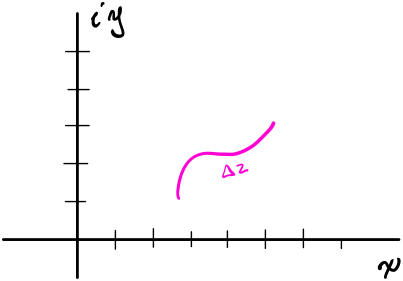
\includegraphics[width=0.3\linewidth]{./media/CompexIntegrals/handwriting.png}



	\label{fig:handwriting}
\end{figure}

this short curve is what we call a contour, the complex integral will be a line integral along that curve:


\begin{figure}[h!]
	\centering
	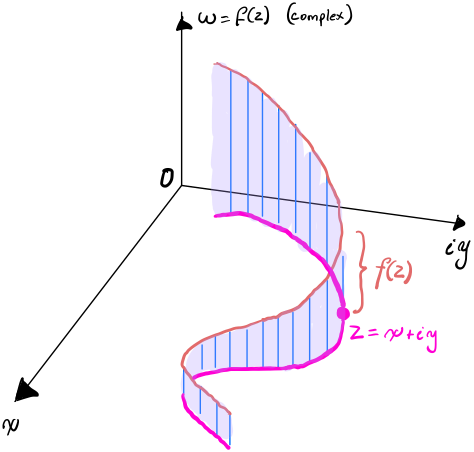
\includegraphics[width=0.3\linewidth]{"./media/CompexIntegrals/handwriting2.png"}
	\caption{}
	\label{fig:handwriting-2}
\end{figure}


\newpage


\paragraph{Define Contours}\ \\
A set of points $z =  \left( x,y \right)$ in the complex plane is said to be an \textbf{\textit{arc}} or a curve that we will call $C$ if:

\begin{align}
 x =  x\left( t \right), \quad y =  y\left( t \right) \qquad \left( a \leq t \leq b \right)
  \label{arcdef}
\end{align}

where:
\begin{itemize}
  \item $x\left( t \right)$ and $y\left( t \right) $ are continuous functions 
    \subitem continuous however does not mean smooth/differentiable, sharp points are allowed.
  \item the output values are ordered corresponding to $t$ (as if $t$ represented time)
\end{itemize}

It is more convenient to describe the curve at (\ref{arcdef}) as:

\begin{align}
  z &= z\left( t \right)  \label{arccompdef} \\
  &= x\left( t \right) + i\cdot y\left( t \right) \notag
\end{align}

\subparagraph{Types of Arcs}\ \\
\begin{itemize}
  \item A \textbf{Simple Curve} does not cross itself
  \item a \textbf{Closed Curve} meets back up with itself
  \item a \textbf{Simple Closed Curve} is closed and does not cross itself (except where it closes)
  \item a \textbf{Positive Curve} moves counter-clockwise as $t$ increases.
\end{itemize}
\begin{figure}[h!]
	
	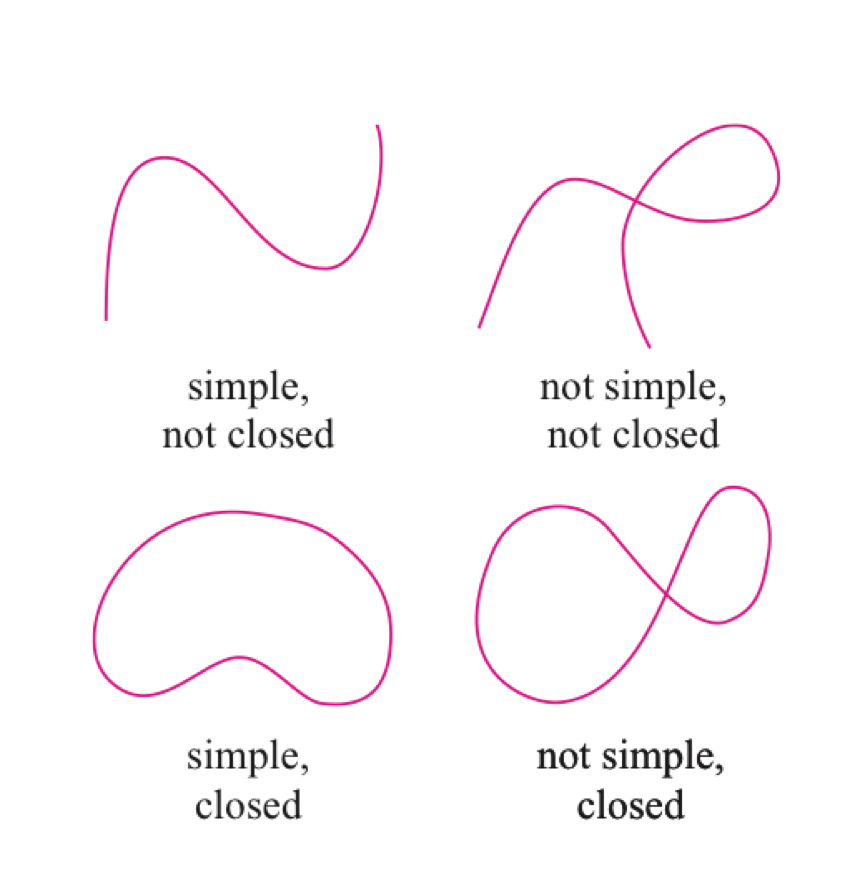
\includegraphics[width=0.2\linewidth]{"./media/CompexIntegrals/Image.png"}

	\label{fig:image}
\end{figure}

\subparagraph{Parametric Representation not unique}\ \\
Also the parametric representation of such a curve is not unique, the same curve could be represented by lots of different parametric equations, just like a second degree polynomial can also be modelled by a 3rd degree polynomial between intervals.

\newpage


\section{Contour Integral}
As previously discussed, an integral with respect to $z$ will be a contour integral:
\[
\int^{}_{C} f \left(z \right)   \operatorname{d}z 
\]
If the value of the integral does not depend on the path of the contour and only depends on the endpoints then we would write:

\[
\int^{}_{C} f \left(z \right)   \operatorname{d}z = \int^{z_2}_{z_1} f\left( z   \right) \operatorname{d}z 
\]
We can also put the integral in terms of the contour parameters, This is basically \textit{Integration by Substitution} in reverse, there's a more rigorous proof in the textbook by \textit{Osbourne}, just take it as definition.

  \begin{align}
    \int^{}_{C}\left( f\left( z \right)  \right) \operatorname{d}z = \int^{b}_{a}\left(f \left[ z\left( t \right)  \right]\cdot  z'\left( t \right)  \right) \operatorname{d}t  
    \label{tdef}
  \end{align}
  
\paragraph{Negative Contours}\ \\
If a contour $C$ is given the contour $- C$ denotes the same contour with the order of the points reversed.
Hence we have:

\begin{align*}
\int^{}_{-C}\left( f\left( z \right)  \right) \operatorname{d}z  &= \int^{- a}_{- b}\left( f\left[ z\left( - t \right)  \right] \cdot \frac{\operatorname{d} }{\operatorname{d} t}\left( z\left( - t \right)  \right)  \right) \operatorname{d}t \\
    &= - \int^{b}_{a}\left( f\left[ z\left( - t \right)  \right] z'\left( - t \right)  \right) \operatorname{d}t \\
    &= - \int^{}_{C}\left( f\left( z \right)  \right) \operatorname{d}z 
\end{align*}


Refer to p. 128 of \textit{Churchill's 9th} for worked examples.

\subsection{Notation}
If we want to basically i want to know does the symbol:
\[
\oint^{}_{} f\left( z \right)   \operatorname{d}z
\]
\begin{itemize}
  \item a contour/line integral of any sort
  \item a contour/line integral around a closed path
  \item one of the above but specifically in the anticlockwise direction?
\end{itemize}

\subsection{Upper Bounds for Moduli}

Start with the triangle inequality:
\[
    \left| \alpha + \beta \right| \leq     \left| \alpha \right| +     \left| \beta \right| 
\]
We could prove this, or, by similar reasoning:

\begin{align*}
\implies      \left| \int^{}_{}\left( w\left(  t \right)  \right) \operatorname{d}t  \right| &\leq \int^{}_{} \left| w\left( t  \right|  \right) \operatorname{d}t 
\end{align*}

   Now let:
   \begin{itemize}
     \item $C$ be a contour of length $L$
     \item  $    \left| f\left( z \right)  \right| \leq M$
   \end{itemize}

   Using the inequality above it can be rigorously shown:

   \[
       \left| \int^{}_{}\left( f\left( z \right)  \right) \operatorname{d}z  \right| \leq M\cdot L
   \]

   This can be somewhat visualised if $f\left( z \right) $ is taken to be the height of the function along the contour, and $L$ is taken to be the length of the contour, although the values will be complex and height might become an odd concept, the mathematics should still hold.
   \paragraph{Example}
   Evaluate the contour integral:
   \[
     \int^{}_{C}\left( \frac{1}{z} \right) \operatorname{d}z 
   \]
   Where:
\begin{itemize}
     \item $C:     \left| z \right| = 1$
\end{itemize}

\noindent   Now put the integral in terms of the parametric representation (\ref{tdef}):

   \begin{align}
       \int^{}_{C}\left( \frac{1}{z} \right) \operatorname{d}z &=  \int^{\pi}_{\pi}\left( \frac{1}{e^{i\theta}} \cdot \frac{\operatorname{d} }{\operatorname{d} \theta}\left( e^{i\theta} \right)  \right) \operatorname{d}\theta \notag \\
       &= \int^{\pi}_{\pi}\left( \frac{1}{e^{i\theta}} \cdot i\cdot e^{i\theta} \right) \operatorname{d}\theta \notag \\
       &= \int^{\pi}_{\pi}\left( i \right) \operatorname{d}\theta \notag \\  
       &= \left[ i \cdot \theta \right]^{\pi}_{\pi} \notag \\
       &= 0
     \label{excontint1}
   \end{align}

   \section{Antiderivatives}
   Generally the value of a contour integral depends on both the path of the contour and the function.\\
   Some contour intergrals however have values independent of the path, for example consider how many integrals over closed paths will have an integral of zero as in the example above.\\

   The antiderivative of a complex function is $F\left( z \right) $ such that:
   \[
   F'\left( z \right) = f\left( z \right) 
   \]
   The antiderivative is, of necessity, an analytic function.

   The antiderivative is uniqe, there is only one antiderivative for a given funciton (other than the additive constant $\left( +  C \right) $ component).

   \subsection{Basic Antiderivative Theorem}
   Suppose $f\left( z \right) $ is continuous in a domain, if the function has an antiderivative $F\left( z \right) $ through the domain then:

   \ \
   
   \hfill\begin{minipage}{\dimexpr\textwidth-3cm}
   integrals of $f\left( z \right) $ along contours lying in the domain depend only on the endpoints of that contour:
   \[
     \int^{}_{C}f\left( z \right)  \operatorname{d}z = \int^{z_2}_{z_1} f\left( z \right)   \operatorname{d}z = \left[ F\left( z \right)  \right]^{z_2}_{z_1} 
   \]

   This also means that integrals around a closed contour will be 0.
   \end{minipage}
   \ \
   

   \paragraph{Proof}
   if $F'\left( z \right)  = f\left( z \right) $ :
   
   \begin{align*}
       \int^{}_{C} f\left( z \right)   \operatorname{d}z &=  \int^{b}_{a} f\left( z\left( t \right)  \right)   \operatorname{d}t \\
       &= \int^{b}_{a} U\left( z\left( t \right)  \right)   \operatorname{d}t + i\cdot \int^{b}_{a} b\left( z\left( t \right)  \right)   \operatorname{d}t\\
       \intertext{Which means the Fundamental Theorem of Calculus Applies from (\ref{ftcest})}
       &= F\left( z\left( b \right)  \right) - F\left( z\left( a \right)  \right) \\
       &=  F\left( z_2 \right) - F\left( z_1 \right) \\
       &= \left[ F\left( z \right)  \right]^{z_2}_{z_1} \\
       &= \left[ U\left( t \right)  \right]^{b}_{a} +  i \cdot  \left[ V\left( t \right)  \right]^{b}_{a} \\
       &= U\left( b \right) - U\left( a \right) +  i \cdot  \left[ V\left( b \right) - V\left( a \right)  \right] \\
       &= \left[ U\left( b \right)+  V\left( b   \right)  \right] -  i \cdot  \left[ U\left( a \right) - V\left( b \right)  \right] \\
       &= F\left( b \right) - F\left( a \right) \\
       &= \left[ F\left( z \right)  \right]^{b}_{a}\\
       &= \left[ F\left( z \right)  \right]^{z_2}_{z_1}
   \end{align*}

   \section{Cauchy Goursat Theorem}
   This theorem depends on \textit{Green's Theorem} which gives the relationship between a line integral around a simple-closed curve and the double integral over the corresponding bounded region, for purely real functions. Roughly Speaking \textit{Green's Theorem} is a counterpart of the Fundamental Theorem of Calculus for double integrals.\\

   In establishing the \textit{Cauchy-Goursat Theorem}, proving \textit{Green's Theorem} is the tricky part, the \textit{Cauchy-Goursat Theorem}  more or less falls out of it. 

\ \

\hfill\begin{minipage}{\dimexpr\textwidth-3cm}
\begin{tcolorbox}

  \subparagraph{ the \textit{Cauchy-Goursat Theorem}} 

  If a function $f$ is analytic at all points interior to, and on, a simple closed contour $C$, then:

  \[
  \oint^{}_{C} f\left( z \right)   \operatorname{d}z = 0 
  \]
\end{tcolorbox}

\end{minipage}
\ \

\subsection{Simply-Connected Domains}
If $f\left( z \right) $ is analytic through a simply connected domain:
\[
\int^{}_{C} f\left( z \right)   \operatorname{d}z 
\]
Where:
\begin{itemize}
  \item C is any closed contour in that domain (Simple or not)
    \subitem i.e. if the domain is simply connected, the contour can cross itself.
\end{itemize}

From this it follows:
\begin{itemize}
  \item If a function is analytic on a simply connected domain, then:
    \subitem there will be an anti-derivative:
    \subsubitem The contour integral will be independent of path (i.e.$F(b) - F(a)$ 
    \item Entire functions always have an antiderivative
      \subitem and will always be independent of path.
\end{itemize}

\subsection{Multiply Connected Domains}
If $C$ is a closed counter-clockwise contour, inside which are closed Clockwise contours $c_1, c_2, c_3 \dots$ for which the function is analytic interior to C but exterior to $c_1, c_2, c_3 \dots$ :


\begin{figure}[h!]
	\centering
	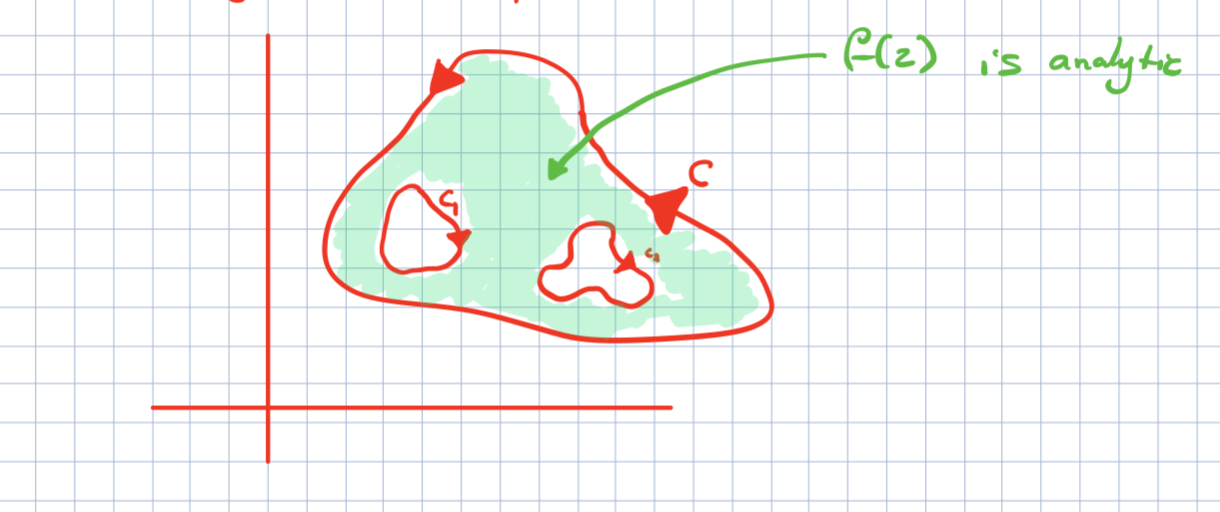
\includegraphics[width=0.7\linewidth]{./media/CompexIntegrals/s1.png}
	\caption{}
	\label{fig:s1}
\end{figure}



Then we have:

\[
\int^{}_{C} f\left( z \right)   \operatorname{d}z + \sum^{k}_{n= 1} \left[ \int^{}_{c_n} f\left( z \right)   \operatorname{d}z  \right] 
\]
This is established by drawing a line through all the interior closed contours and applying the \textit{Cauchy-Goursat} theorem, refer to the \textit{Churchill} textbook.

\paragraph{Principle of Deformation}
If we had Something like this:

\begin{figure}[h!]
	\centering
	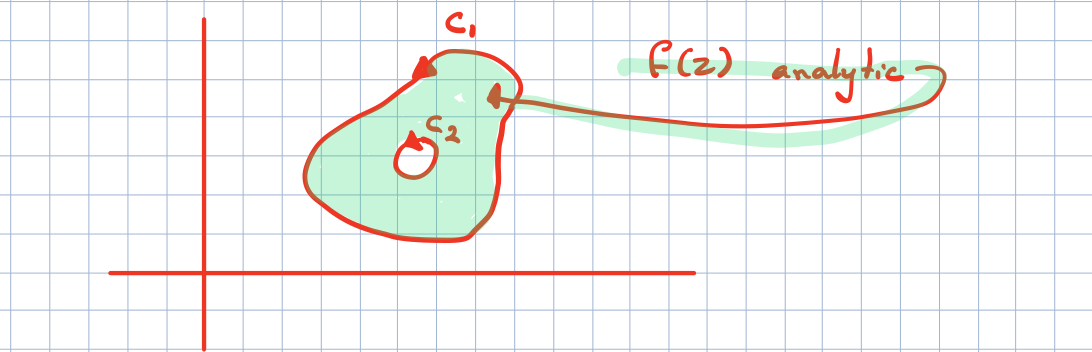
\includegraphics[width=0.7\linewidth]{./media/CompexIntegrals/s2.png}
	\caption{}
	\label{fig:s2}
\end{figure}


Then it would follow:

\begin{align*}
  \int^{}_{C_1} f\left( z \right)   \operatorname{d}z + \int^{}_{c_2} f\left( z \right)   \operatorname{d}z &= 0\\  
  \int^{}_{C_1} f\left( z \right)   \operatorname{d}z - \int^{}_{c_2} f\left( z \right)   \operatorname{d}z &= 0\\
  \int^{}_{C_1} f\left( z \right)   \operatorname{d}z &= \int^{}_{c_2} f\left( z \right)   \operatorname{d}z  
\end{align*}

So if $c_2$ can be continuously transformed into $C_1$ through an analytic region, then the integral is the same.

\subparagraph{Spacial Case of Deformation}
We Should Probably memorise this special case:

\[
\ointctrclockwise^{}_{    \left| z - z_0 \right| = r} \left( z- z_0 \right) ^n  \operatorname{d}z = 
\begin{cases}
  0 \qquad if n \neq - 1\\
  2\pi i \qquad if n = - 12
\end{cases}
\]

\subparagraph{Example}

\begin{align*}
    \int^{}_{    \left| z \right| = 1} \frac{1}{z^2 +  2z+2 }  \operatorname{d}z &= \int^{}_{    \left| z \right| = 1} \frac{1}{\left( z +  \left( 1 +  i \right)  \right) \cdot \left( z +  \left( 1 -  i \right)  \right) }  \operatorname{d}z  \\
    \intertext{There is a singularity at $z =  - 1 \pm i$, which is outside the closed countour, the function is analytic everwhere else inside and on the closed countour hence by the \textit{Cauchy-Goursatt Theorem:}}\\
  \int^{}_{    \left| z \right| = 1} \frac{1}{z^2 +  2z +  2}  \operatorname{d}z &= 0 
\end{align*}

\section{Cauchy Integral Formula}
This has to be memorised.\ \\

\hfill\begin{minipage}{\dimexpr\textwidth-3cm}
\begin{tcolorbox}

  \subparagraph{Cauchy Integral Formula}\ \\
If $f$ is analytic everwhere inside and on $C$ and $z_0$ is interior to C:
\[
  \int^{}_{C} \frac{f\left( z \right) }{z - z_0}  \operatorname{d}z = 2\pi i \cdot  f \left( z_0 \right)  
\]
\end{tcolorbox}

\end{minipage}
\ \


\paragraph{Example}
Solve :
\[
\int^{}_{    \left| z \right| = 1} \frac{\cos{z}}{z^3 +  9z}   \operatorname{d}z 
\]
First simplify the intergrand somewhat:

\[
  \int^{}_{    \left| z \right| = 1} \frac{\cos{z}}{z^3 +  9z}  \operatorname{d}z = \int^{}_{    \left| z \right| = 1} \frac{1}{z} \cdot  \frac{\cos{z}}{z^2 +  9z}  \operatorname{d}z  
\]


Observe that the intergrand $\frac{\cos{z}}{z^3 +  9z}$ is analytic everywhere other than its singularities:

\begin{itemize}
  \item $z =  0$ 
  \item $z = 3i$
  \item $z =  - 3i$ 
\end{itemize}


because $z = 0$ is inside the contour we cannot use the \textit{Cauchy-Goursatt Theorem}, however, we can use the \textit{Cauchy-Integral Formula} precisely because :
\begin{itemize}
  \item $z_0 = 0$ is interior to the closed contour
  \item $f\left( z \right) = \frac{\cos{z}}{z^2+ 9} $ is analytic everywhere else interior to the closed contour
\end{itemize}

So by the Cauchy Integral Formula:

\begin{align*}
    \int^{}_{    \left| z \right| = 1} \frac{\frac{\cos{z}}{z^2+ 9}}{\left( z- 0 \right) }  \operatorname{d}z &= 2\pi i \cdot \frac{\cos{\left( 0 \right) }}{0^2+ 9} \\
    &= i\cdot \frac{2\pi}{9}
\end{align*}

\section{Extension of the Cauchy Integral Formula}
This has to be memorised:

 \ \

\hfill\begin{minipage}{\dimexpr\textwidth-3cm}
\begin{tcolorbox}
  \subparagraph{Extension to Cauchy Integral}\ \\

if:
\begin{itemize}
  \item $f\left( z \right) $ is analytic on and interior to some closed contour $C$ 
  \item $z_0$ is interior to $C$ 
\end{itemize}

Then:
\[
  \int^{}_{C} \frac{f\left( z \right) }{\left( z- z_0 \right) ^{n+ 1}}  \operatorname{d}z = f^{n}\left( z_0 \right) \cdot \frac{2\pi i}{n!} 
\]
\end{tcolorbox}

\end{minipage}
\ \




\end{document}

 %\documentclass[class=article, crop=false]{standalone}

\usepackage{./resources/style}
\usepackage{./resources/referencing}

 \title{(10) Complex Integrals}
\date{Analysis (200023)}
\author{Analysis (200023)}
% \usepackage{cancel}
% \usepackage{geometry}
% \geometry{a4paper, portrait, margin=1in}
% \usepackage{centernot}
% \usepackage{wrapfig}
% \usepackage{amsmath}
% \usepackage{esint}
% \usepackage{steinmetz}
% \usepackage{lipsum}% http://ctan.org/pkg/lipsum
% \usepackage{amssymb}
% \usepackage{lmodern}
% \usepackage{graphicx}
% \usepackage{amsfonts}
% \usepackage{xfrac}
% %%Bookmarks does the PDF outline and \tableofcontents
% \usepackage[colorlinks=true,linkcolor=blue,urlcolor=black,bookmarksopen=true]{hyperref}
% \usepackage[depth=5]{bookmark}% Show up to level 4 (\paragraph) in bookmarks
% \setcounter{tocdepth}{3}% Show up to level 3 (\subsubsection) in ToC
% \usepackage{titlesec} %This is to stop the automatic numbering of sections (you can't use * with TOC)
% \usepackage[most]{tcolorbox} %Theorem Boxes
% \titleformat{\chapter}[display] %No Numbering for chapter
%   {\normalfont\bfseries}{}{0pt}{\Huge}
%
% %%Fix Headers Otherwise it has half an erroneous number in there
% \usepackage{fancyhdr}
% \pagestyle{fancy}
% %\fancyhf{}
% %\fancyhead[R]{\leftmark}
% %\fancyhead[L]{\rightmark}
% %\renewcommand\headrulewidth{0pt}
% %\renewcommand\chaptermark[1]{\markboth{#1}{}}
% %\renewcommand\sectionmark[1]{\markright{\thesection.\ #1}}
% \rhead[\rightmark]{\rightmark}
% \lhead[(8) Integrals]{(8) Integrals}
% %\fancyhead[R]{\rightmark}
%
% %%Stop Numbers for Sections
%
% \renewcommand{\thesection}{\hspace*{-1.0em}}
% \renewcommand{\thesubsection}{}
% \renewcommand{\thechapter}{}
% \renewcommand{\theequation}{\arabic{equation}}
%
% %% Get rid of the heading for the TOC
%
% \newtcbtheorem{Theorem}{Theorem}{
%   enhanced,
%   sharp corners,
%   attach boxed title to top left={
%     yshifttext=-1mm
%   },
%   colback=white,
%   colframe=blue!75!black,
%   fonttitle=\bfseries,
%   boxed title style={
%     sharp corners,
%     size=small,
%     colback=blue!75!black,
%     colframe=blue!75!black,
%   }
% }{thm}
% \newtcbtheorem[no counter]{Proof}{Proof}{
%   enhanced,
%   sharp corners,
%   attach boxed title to top left={
%     yshifttext=-1mm
%   },
%   colback=white,
%   colframe=blue!25,
%   fonttitle=\bfseries,
%   coltitle=black,
%   boxed title style={
%     sharp corners,
%     size=small,
%     colback=blue!25,
%     colframe=blue!25,
%   }
% }{prf}

\title{(10) Integrals}
\author{Analysis (200023)}


\begin{document}
	\maketitle
	\tableofcontents
	
        \section{Integrals from a Real Domain}
        To begin this consider the function:
        \[
        w: \mathbb{R}     \rightarrow \mathbb{C}  
        \]
        we can decompose such a function into real and imaginary components:
        \[
          w \left( t \right) =  u \left( t \right) +  i \cdot  v \left( t \right) 
        \]
        where $u$ and $v$ are purely real functions.
        \subsection{Differentiation}
        If $w =  f \left( z \right) $:
        \[
          f' \left( z \right) = \frac{\operatorname{d}w }{\operatorname{d} z} \quad \text{(As if $z$ was a purely real operator)}
        \]
        If $g\left( x,y \right)  =  u\left(  x,y  \right)  +  i \cdot  v \left( x, y \right) $: 

        \begin{align*}
        f'\left( z \right) &= \frac{\partial u }{\partial x}+ \frac{\partial v }{\partial x} \\
        &= \frac{dw}{dz}
        \end{align*}

        If $w =  u\left( t \right) + i \cdot v \left( t \right) $:
        \[
        w'\left( t \right) =  \frac{\operatorname{d}u }{\operatorname{d} t} + i \cdot \frac{\operatorname{d} v}{\operatorname{d} t}
        \]

        \subsection{Integration}
        If $w =  u\left( t \right) + i \cdot v \left( t \right) $:


        \[
        \int^{b}_{a}\left( w \left( t \right)  \right) \operatorname{d}t =  \int^{b}_{a}\left( u \right) \operatorname{d}t + i \cdot  \int^{ b}_{a}\left( v \right) \operatorname{d}t   
        \]

        \paragraph{Fundamental Theorem of Calculus} \ \\
        The fundamental theorem of calculus applies here:
        \begin{align}
         \int^{b}_{a}\left( w\left( t \right)  \right) \operatorname{d}t =  \left[ W\left( t \right)  \right]^b_a 
          \label{ftcest}
        \end{align}
        \subparagraph{Justification}

        let $W\left( t \right) =  U\left( t \right) +  i \cdot  V\left( t \right) $ be the antiderivative of $w\left( t \right) $:

        \begin{align*}
          \int^{b}_{a}\left( w \left( t \right)  \right) \operatorname{d}t &= \left[ U\left( t \right)  \right]^b_a + i\cdot \left[ v\left( t \right)  \right]^b_a \\
          &= \left[ U\left( b \right) + i\cdot V\left( b \right)  \right] -\left[ U\left( a \right) +  i \cdot V\left( a \right)  \right]  \\
          &= \left[ W\left( b \right) - W\left( a \right)  \right] \\
          &= \left[ W\left( t \right)  \right]^b_a
        \end{align*}
        \begin{flushright}
        {\rule{0.7em}{0.7em}}
        \end{flushright}
         
        \section{Contours}
        Integrals of complex valued functions are of the form:
        \[
          \lim_{n     \rightarrow \infty}\left( \sum^{n}_{i= 1}\left[ f\left( z^*_i \right) \cdot \Delta z \right]  \right)
        \]
         $\Delta z$ could be along any curve in the complex plane rather than just the axis along which we would integrate:
        
\begin{figure}[h!]
	
	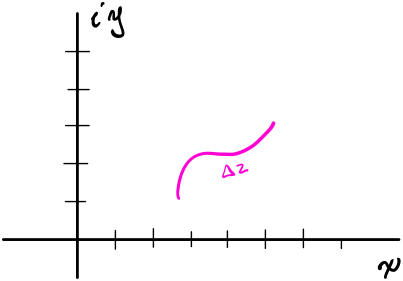
\includegraphics[width=0.3\linewidth]{./media/CompexIntegrals/handwriting.png}



	\label{fig:handwriting}
\end{figure}

this short curve is what we call a contour, the complex integral will be a line integral along that curve:


\begin{figure}[h!]
	\centering
	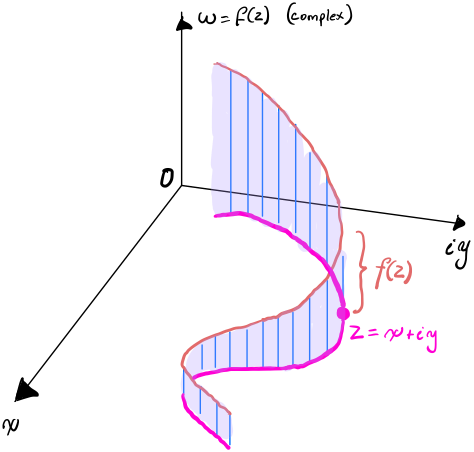
\includegraphics[width=0.3\linewidth]{"./media/CompexIntegrals/handwriting2.png"}
	\caption{}
	\label{fig:handwriting-2}
\end{figure}


\newpage


\paragraph{Define Contours}\ \\
A set of points $z =  \left( x,y \right)$ in the complex plane is said to be an \textbf{\textit{arc}} or a curve that we will call $C$ if:

\begin{align}
 x =  x\left( t \right), \quad y =  y\left( t \right) \qquad \left( a \leq t \leq b \right)
  \label{arcdef}
\end{align}

where:
\begin{itemize}
  \item $x\left( t \right)$ and $y\left( t \right) $ are continuous functions 
    \subitem continuous however does not mean smooth/differentiable, sharp points are allowed.
  \item the output values are ordered corresponding to $t$ (as if $t$ represented time)
\end{itemize}

It is more convenient to describe the curve at (\ref{arcdef}) as:

\begin{align}
  z &= z\left( t \right)  \label{arccompdef} \\
  &= x\left( t \right) + i\cdot y\left( t \right) \notag
\end{align}

\subparagraph{Types of Arcs}\ \\
\begin{itemize}
  \item A \textbf{Simple Curve} does not cross itself
  \item a \textbf{Closed Curve} meets back up with itself
  \item a \textbf{Simple Closed Curve} is closed and does not cross itself (except where it closes)
  \item a \textbf{Positive Curve} moves counter-clockwise as $t$ increases.
\end{itemize}
\begin{figure}[h!]
	
	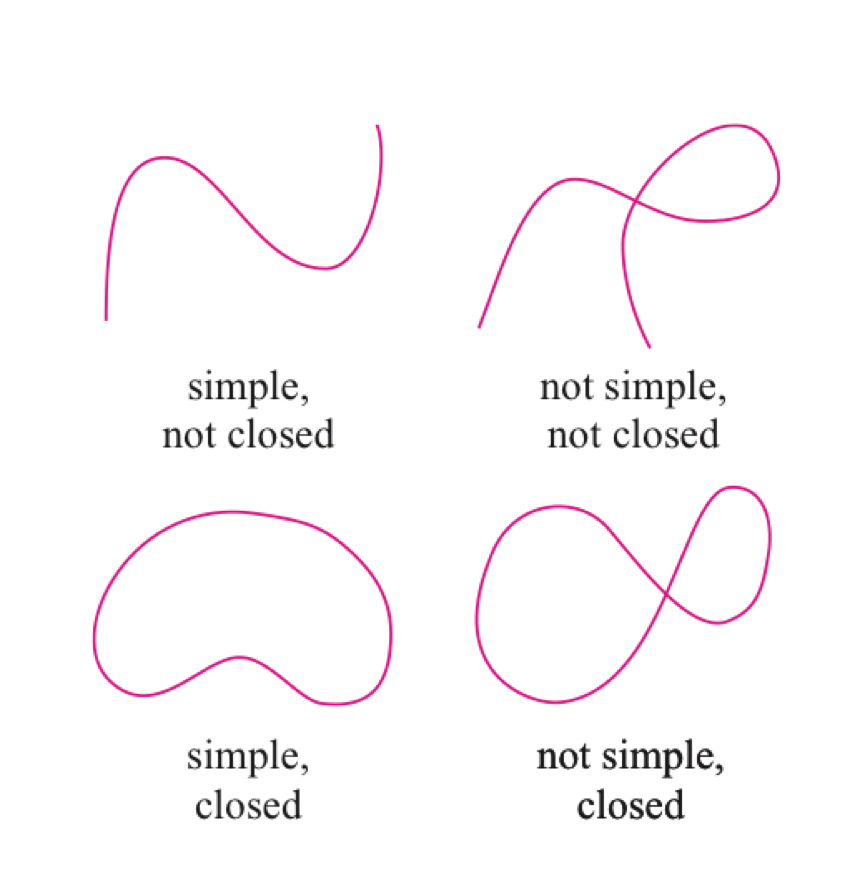
\includegraphics[width=0.2\linewidth]{"./media/CompexIntegrals/Image.png"}

	\label{fig:image}
\end{figure}

\subparagraph{Parametric Representation not unique}\ \\
Also the parametric representation of such a curve is not unique, the same curve could be represented by lots of different parametric equations, just like a second degree polynomial can also be modelled by a 3rd degree polynomial between intervals.

\newpage


\section{Contour Integral}
As previously discussed, an integral with respect to $z$ will be a contour integral:
\[
\int^{}_{C} f \left(z \right)   \operatorname{d}z 
\]
If the value of the integral does not depend on the path of the contour and only depends on the endpoints then we would write:

\[
\int^{}_{C} f \left(z \right)   \operatorname{d}z = \int^{z_2}_{z_1} f\left( z   \right) \operatorname{d}z 
\]
We can also put the integral in terms of the contour parameters, This is basically \textit{Integration by Substitution} in reverse, there's a more rigorous proof in the textbook by \textit{Osbourne}, just take it as definition.

  \begin{align}
    \int^{}_{C}\left( f\left( z \right)  \right) \operatorname{d}z = \int^{b}_{a}\left(f \left[ z\left( t \right)  \right]\cdot  z'\left( t \right)  \right) \operatorname{d}t  
    \label{tdef}
  \end{align}
  
\paragraph{Negative Contours}\ \\
If a contour $C$ is given the contour $- C$ denotes the same contour with the order of the points reversed.
Hence we have:

\begin{align*}
\int^{}_{-C}\left( f\left( z \right)  \right) \operatorname{d}z  &= \int^{- a}_{- b}\left( f\left[ z\left( - t \right)  \right] \cdot \frac{\operatorname{d} }{\operatorname{d} t}\left( z\left( - t \right)  \right)  \right) \operatorname{d}t \\
    &= - \int^{b}_{a}\left( f\left[ z\left( - t \right)  \right] z'\left( - t \right)  \right) \operatorname{d}t \\
    &= - \int^{}_{C}\left( f\left( z \right)  \right) \operatorname{d}z 
\end{align*}


Refer to p. 128 of \textit{Churchill's 9th} for worked examples.

\subsection{Notation}
If we want to basically i want to know does the symbol:
\[
\oint^{}_{} f\left( z \right)   \operatorname{d}z
\]
\begin{itemize}
  \item a contour/line integral of any sort
  \item a contour/line integral around a closed path
  \item one of the above but specifically in the anticlockwise direction?
\end{itemize}

\subsection{Upper Bounds for Moduli}

Start with the triangle inequality:
\[
    \left| \alpha + \beta \right| \leq     \left| \alpha \right| +     \left| \beta \right| 
\]
We could prove this, or, by similar reasoning:

\begin{align*}
\implies      \left| \int^{}_{}\left( w\left(  t \right)  \right) \operatorname{d}t  \right| &\leq \int^{}_{} \left| w\left( t  \right|  \right) \operatorname{d}t 
\end{align*}

   Now let:
   \begin{itemize}
     \item $C$ be a contour of length $L$
     \item  $    \left| f\left( z \right)  \right| \leq M$
   \end{itemize}

   Using the inequality above it can be rigorously shown:

   \[
       \left| \int^{}_{}\left( f\left( z \right)  \right) \operatorname{d}z  \right| \leq M\cdot L
   \]

   This can be somewhat visualised if $f\left( z \right) $ is taken to be the height of the function along the contour, and $L$ is taken to be the length of the contour, although the values will be complex and height might become an odd concept, the mathematics should still hold.
   \paragraph{Example}
   Evaluate the contour integral:
   \[
     \int^{}_{C}\left( \frac{1}{z} \right) \operatorname{d}z 
   \]
   Where:
\begin{itemize}
     \item $C:     \left| z \right| = 1$
\end{itemize}

\noindent   Now put the integral in terms of the parametric representation (\ref{tdef}):

   \begin{align}
       \int^{}_{C}\left( \frac{1}{z} \right) \operatorname{d}z &=  \int^{\pi}_{\pi}\left( \frac{1}{e^{i\theta}} \cdot \frac{\operatorname{d} }{\operatorname{d} \theta}\left( e^{i\theta} \right)  \right) \operatorname{d}\theta \notag \\
       &= \int^{\pi}_{\pi}\left( \frac{1}{e^{i\theta}} \cdot i\cdot e^{i\theta} \right) \operatorname{d}\theta \notag \\
       &= \int^{\pi}_{\pi}\left( i \right) \operatorname{d}\theta \notag \\  
       &= \left[ i \cdot \theta \right]^{\pi}_{\pi} \notag \\
       &= 0
     \label{excontint1}
   \end{align}

   \section{Antiderivatives}
   Generally the value of a contour integral depends on both the path of the contour and the function.\\
   Some contour intergrals however have values independent of the path, for example consider how many integrals over closed paths will have an integral of zero as in the example above.\\

   The antiderivative of a complex function is $F\left( z \right) $ such that:
   \[
   F'\left( z \right) = f\left( z \right) 
   \]
   The antiderivative is, of necessity, an analytic function.

   The antiderivative is uniqe, there is only one antiderivative for a given funciton (other than the additive constant $\left( +  C \right) $ component).

   \subsection{Basic Antiderivative Theorem}
   Suppose $f\left( z \right) $ is continuous in a domain, if the function has an antiderivative $F\left( z \right) $ through the domain then:

   \ \
   
   \hfill\begin{minipage}{\dimexpr\textwidth-3cm}
   integrals of $f\left( z \right) $ along contours lying in the domain depend only on the endpoints of that contour:
   \[
     \int^{}_{C}f\left( z \right)  \operatorname{d}z = \int^{z_2}_{z_1} f\left( z \right)   \operatorname{d}z = \left[ F\left( z \right)  \right]^{z_2}_{z_1} 
   \]

   This also means that integrals around a closed contour will be 0.
   \end{minipage}
   \ \
   

   \paragraph{Proof}
   if $F'\left( z \right)  = f\left( z \right) $ :
   
   \begin{align*}
       \int^{}_{C} f\left( z \right)   \operatorname{d}z &=  \int^{b}_{a} f\left( z\left( t \right)  \right)   \operatorname{d}t \\
       &= \int^{b}_{a} U\left( z\left( t \right)  \right)   \operatorname{d}t + i\cdot \int^{b}_{a} b\left( z\left( t \right)  \right)   \operatorname{d}t\\
       \intertext{Which means the Fundamental Theorem of Calculus Applies from (\ref{ftcest})}
       &= F\left( z\left( b \right)  \right) - F\left( z\left( a \right)  \right) \\
       &=  F\left( z_2 \right) - F\left( z_1 \right) \\
       &= \left[ F\left( z \right)  \right]^{z_2}_{z_1} \\
       &= \left[ U\left( t \right)  \right]^{b}_{a} +  i \cdot  \left[ V\left( t \right)  \right]^{b}_{a} \\
       &= U\left( b \right) - U\left( a \right) +  i \cdot  \left[ V\left( b \right) - V\left( a \right)  \right] \\
       &= \left[ U\left( b \right)+  V\left( b   \right)  \right] -  i \cdot  \left[ U\left( a \right) - V\left( b \right)  \right] \\
       &= F\left( b \right) - F\left( a \right) \\
       &= \left[ F\left( z \right)  \right]^{b}_{a}\\
       &= \left[ F\left( z \right)  \right]^{z_2}_{z_1}
   \end{align*}

   \section{Cauchy Goursat Theorem}
   This theorem depends on \textit{Green's Theorem} which gives the relationship between a line integral around a simple-closed curve and the double integral over the corresponding bounded region, for purely real functions. Roughly Speaking \textit{Green's Theorem} is a counterpart of the Fundamental Theorem of Calculus for double integrals.\\

   In establishing the \textit{Cauchy-Goursat Theorem}, proving \textit{Green's Theorem} is the tricky part, the \textit{Cauchy-Goursat Theorem}  more or less falls out of it. 

\ \

\hfill\begin{minipage}{\dimexpr\textwidth-3cm}
\begin{tcolorbox}

  \subparagraph{ the \textit{Cauchy-Goursat Theorem}} 

  If a function $f$ is analytic at all points interior to, and on, a simple closed contour $C$, then:

  \[
  \oint^{}_{C} f\left( z \right)   \operatorname{d}z = 0 
  \]
\end{tcolorbox}

\end{minipage}
\ \

\subsection{Simply-Connected Domains}
If $f\left( z \right) $ is analytic through a simply connected domain:
\[
\int^{}_{C} f\left( z \right)   \operatorname{d}z 
\]
Where:
\begin{itemize}
  \item C is any closed contour in that domain (Simple or not)
    \subitem i.e. if the domain is simply connected, the contour can cross itself.
\end{itemize}

From this it follows:
\begin{itemize}
  \item If a function is analytic on a simply connected domain, then:
    \subitem there will be an anti-derivative:
    \subsubitem The contour integral will be independent of path (i.e.$F(b) - F(a)$ 
    \item Entire functions always have an antiderivative
      \subitem and will always be independent of path.
\end{itemize}

\subsection{Multiply Connected Domains}
If $C$ is a closed counter-clockwise contour, inside which are closed Clockwise contours $c_1, c_2, c_3 \dots$ for which the function is analytic interior to C but exterior to $c_1, c_2, c_3 \dots$ :


\begin{figure}[h!]
	\centering
	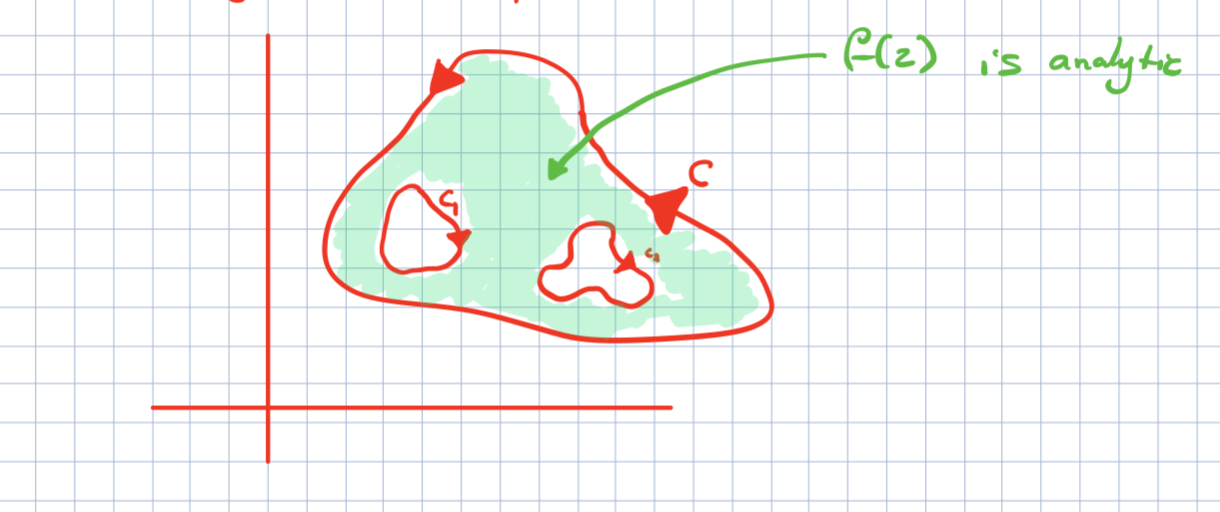
\includegraphics[width=0.7\linewidth]{./media/CompexIntegrals/s1.png}
	\caption{}
	\label{fig:s1}
\end{figure}



Then we have:

\[
\int^{}_{C} f\left( z \right)   \operatorname{d}z + \sum^{k}_{n= 1} \left[ \int^{}_{c_n} f\left( z \right)   \operatorname{d}z  \right] 
\]
This is established by drawing a line through all the interior closed contours and applying the \textit{Cauchy-Goursat} theorem, refer to the \textit{Churchill} textbook.

\paragraph{Principle of Deformation}
If we had Something like this:

\begin{figure}[h!]
	\centering
	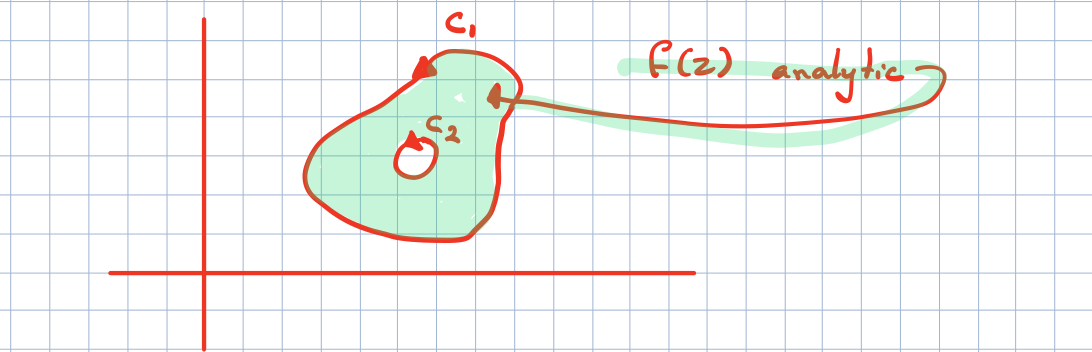
\includegraphics[width=0.7\linewidth]{./media/CompexIntegrals/s2.png}
	\caption{}
	\label{fig:s2}
\end{figure}


Then it would follow:

\begin{align*}
  \int^{}_{C_1} f\left( z \right)   \operatorname{d}z + \int^{}_{c_2} f\left( z \right)   \operatorname{d}z &= 0\\  
  \int^{}_{C_1} f\left( z \right)   \operatorname{d}z - \int^{}_{c_2} f\left( z \right)   \operatorname{d}z &= 0\\
  \int^{}_{C_1} f\left( z \right)   \operatorname{d}z &= \int^{}_{c_2} f\left( z \right)   \operatorname{d}z  
\end{align*}

So if $c_2$ can be continuously transformed into $C_1$ through an analytic region, then the integral is the same.

\subparagraph{Spacial Case of Deformation}
We Should Probably memorise this special case:

\[
\ointctrclockwise^{}_{    \left| z - z_0 \right| = r} \left( z- z_0 \right) ^n  \operatorname{d}z = 
\begin{cases}
  0 \qquad if n \neq - 1\\
  2\pi i \qquad if n = - 12
\end{cases}
\]

\subparagraph{Example}

\begin{align*}
    \int^{}_{    \left| z \right| = 1} \frac{1}{z^2 +  2z+2 }  \operatorname{d}z &= \int^{}_{    \left| z \right| = 1} \frac{1}{\left( z +  \left( 1 +  i \right)  \right) \cdot \left( z +  \left( 1 -  i \right)  \right) }  \operatorname{d}z  \\
    \intertext{There is a singularity at $z =  - 1 \pm i$, which is outside the closed countour, the function is analytic everwhere else inside and on the closed countour hence by the \textit{Cauchy-Goursatt Theorem:}}\\
  \int^{}_{    \left| z \right| = 1} \frac{1}{z^2 +  2z +  2}  \operatorname{d}z &= 0 
\end{align*}

\section{Cauchy Integral Formula}
This has to be memorised.\ \\

\hfill\begin{minipage}{\dimexpr\textwidth-3cm}
\begin{tcolorbox}

  \subparagraph{Cauchy Integral Formula}\ \\
If $f$ is analytic everwhere inside and on $C$ and $z_0$ is interior to C:
\[
  \int^{}_{C} \frac{f\left( z \right) }{z - z_0}  \operatorname{d}z = 2\pi i \cdot  f \left( z_0 \right)  
\]
\end{tcolorbox}

\end{minipage}
\ \


\paragraph{Example}
Solve :
\[
\int^{}_{    \left| z \right| = 1} \frac{\cos{z}}{z^3 +  9z}   \operatorname{d}z 
\]
First simplify the intergrand somewhat:

\[
  \int^{}_{    \left| z \right| = 1} \frac{\cos{z}}{z^3 +  9z}  \operatorname{d}z = \int^{}_{    \left| z \right| = 1} \frac{1}{z} \cdot  \frac{\cos{z}}{z^2 +  9z}  \operatorname{d}z  
\]


Observe that the intergrand $\frac{\cos{z}}{z^3 +  9z}$ is analytic everywhere other than its singularities:

\begin{itemize}
  \item $z =  0$ 
  \item $z = 3i$
  \item $z =  - 3i$ 
\end{itemize}


because $z = 0$ is inside the contour we cannot use the \textit{Cauchy-Goursatt Theorem}, however, we can use the \textit{Cauchy-Integral Formula} precisely because :
\begin{itemize}
  \item $z_0 = 0$ is interior to the closed contour
  \item $f\left( z \right) = \frac{\cos{z}}{z^2+ 9} $ is analytic everywhere else interior to the closed contour
\end{itemize}

So by the Cauchy Integral Formula:

\begin{align*}
    \int^{}_{    \left| z \right| = 1} \frac{\frac{\cos{z}}{z^2+ 9}}{\left( z- 0 \right) }  \operatorname{d}z &= 2\pi i \cdot \frac{\cos{\left( 0 \right) }}{0^2+ 9} \\
    &= i\cdot \frac{2\pi}{9}
\end{align*}

\section{Extension of the Cauchy Integral Formula}
This has to be memorised:

 \ \

\hfill\begin{minipage}{\dimexpr\textwidth-3cm}
\begin{tcolorbox}
  \subparagraph{Extension to Cauchy Integral}\ \\

if:
\begin{itemize}
  \item $f\left( z \right) $ is analytic on and interior to some closed contour $C$ 
  \item $z_0$ is interior to $C$ 
\end{itemize}

Then:
\[
  \int^{}_{C} \frac{f\left( z \right) }{\left( z- z_0 \right) ^{n+ 1}}  \operatorname{d}z = f^{n}\left( z_0 \right) \cdot \frac{2\pi i}{n!} 
\]
\end{tcolorbox}

\end{minipage}
\ \




\end{document}

%\input{11_cauchyIntegrals/08_vars (copy).tex}
 %
 \chapter{Cauchy Integral Formula}
 \documentclass[class=article, crop=false]{standalone}

\usepackage{./resources/style}
\usepackage{./resources/referencing}


\title{Deriving the Normal Distribution}
\author{Ryan Greenup}
\date{Autumn 2020}

\begin{document}
\hypertarget{power-series-and-uniform-continuity}{%
\section{Power Series and Uniform
Continuity}\label{power-series-and-uniform-continuity}}

\hypertarget{power-series}{%
\subsection{Power Series}\label{power-series}}

\hypertarget{convergence}{%
\subsubsection{Convergence}\label{convergence}}

A sequence \(x=(x_n)\) converges if:

\begin{align*}
\forall \varepsilon > 0, \quad \exists N:&
\ \\
&n \geq N \implies |x_n - x | < \varepsilon
\end{align*}

and it is hence expressed:

\[
\lim(x_n) = x
\]

A series is generated by a sequence,

If \((a_n)\) is a sequence, the series is \((S_n)\):

\begin{align*}
S_1 &= a_1 \\
s_2&= S_1 +  a_2 \\
S_3&= S_2 +  a_3\\
S_4&= S_3+ a_4\\
\cdots
\end{align*}

The series is convergent if:

\begin{align*}
  \forall \varepsilon > 0, \exists N:&\\
&  n \geq N \ \implies    \left| S_n - L \right|  < \varepsilon
\end{align*}

The series is absolutely convergent if $\left\lvert S_n \right\rvert$ is convergent.

The notation for series used is:

\begin{align*}
\sum^{\infty}_{n=1} \left[ \left( a_n \right)  \right] = \sum \left( a_n \right) = \lim_{}\left[ S_n \right]
\end{align*}

Be mindful that this notation is used ambiguously to represent both:

\begin{itemize}
\item
  The infinite Series
\item
  The limit value of the series.
\end{itemize}

In practice however the ambiguity is a non-issue because context will
discern the difference.

\hypertarget{sequences-of-functionstbook}{%
\subsubsection[Sequences of Functions]{\texorpdfstring{Sequences of
Functions\footnote{This is in the Bartle and Sherbert Textbook at
  Chapter {[}8.1.7{]} p.~246}}{Sequences of Functions}}\label{sequences-of-functionstbook}}

We can have sequences of real numbers, and similarly we can have
sequences of functions.

Sequences of functions can converge in two ways:

\begin{itemize}
\item
  Pointwise
\item
  uniformly
\end{itemize}

Uniform convergence is important because it preserves term properties to
the limit function which will be seen.

\hypertarget{define-a-sequence-of-functions}{%
\paragraph{Define a sequence of
functions:}\label{define-a-sequence-of-functions}}

Let $A \subseteq \mathbb{R} , n \in \mathbb{N}$ and take some
function \(f\) :


\begin{align*}
f_n: A     \rightarrow \mathbb{R}
\end{align*}

 It is said that $\left( f\_n \right)$ is a sequence of functions
on \(A\) to $\mathbb{R}$.

For every \(x \in A\) there will be a sequence of real numbers:


\begin{align*}
f_n\left( x \right)
\end{align*}

 For some values of \(x\), the sequence may converge, for others it
may not.

\begin{itemize}
\item
  The point of convergence is
  \( \lim\_\{\}\left[ f_n\left( x_n \right)  \right] \) which depends on
  the choice of \(x\).
\item
  Thus we could Create a set of all \(x \in A\) forwhich
  \(\left( f_n\left( x \right) \right)\) converges.

  \begin{itemize}
  \item
    This set would be a domain for a function $f\left( x \right)$
    that would act as the limit of the sequence \(\left( f\_n\left( x
    \right) \right) \).
  \end{itemize}
\end{itemize}

\hypertarget{pointwise-convergence}{%
\paragraph{Pointwise Convergence}\label{pointwise-convergence}}

Take some function:

  \begin{align*}
  f: A_0     \rightarrow  \mathbb{R} \qquad \left( A_0 \subseteq A \subseteq \mathbb{R}  \right)
  \end{align*}

We say that the sequence is pointwise convergent if,

\begin{itemize}
\item
  for every \(x \in A_0\)

  \begin{itemize}
  \item
    The sequence \(\left( f\_n\left( x \right) \right) \) converges to
    \(f\left( x \right) \).
  \end{itemize}

  e.g.~\(\ \ \) consider \(g_n\left( x \right) : = x^n\);

  \begin{align*}
    \left( g_n\left( x \right)  \right) = \left( x, x^2, x^3, x^4 \cdots \right)
  \end{align*}
   If \(- 1 < x < 1 \quad\), then $x$ is a fraction or zero so:
  \begin{align*}
    \left( x, x^2, x^3, x^4 \cdots 0 \right) \qquad \text{ Converges to 0}
  \end{align*}

  if \(x = 1\), then:

  \begin{align*}
    \left( x, x^2, x^3 \cdots \right) = \left( 1, 1^2, 1^3, \cdots 1 \right)  \qquad \text{Converges to 1}
    \end{align*}

   if \(x= -1\), then:

  \begin{align*}
    \left( x, x^2, x^3, \cdots \right) = \left( 1, - 1, 1, - 1, \cdots \pm 1 \right) \qquad \text{Divergent}
  \end{align*}


  if \(\left\lvert x \right\rvert > 1\), then:

  \begin{align*}
    \left( x, x^2, x^3, \cdots \infty \right) \qquad \text{Divergent}
  \end{align*}

  So \(\lim\_\{\}\left[ g_n\left( x \right)  \right]\) on the set
  \(\left(- 1, 1\right] \) where:

  \begin{align*}
  g\left( x \right) =
  \begin{cases}
    0, \qquad \text{for} \enspace \left( - 1<x<1 \right) \\
    1,\qquad \text{for} \enspace \left( x = 1 \right)
  \end{cases}
  \end{align*}

\end{itemize}

\hypertarget{definition}{%
\paragraph{Definition}\label{definition}}

An alternative, but equivalent definition for pointwise convergence is:

\begin{align}
  \forall \varepsilon>0, \enspace \forall &x \in A_0, \enspace \exists N:\\
  \ \\
&n \geq N  \implies       \left| f_n\left( x \right)  -  f\left( x \right)  \right| < \varepsilon
\end{align}

Where \(N\) is a function of \(x\) and \(\varepsilon\), i.e.:

\begin{itemize}
\item
  \(N = N\left( \varepsilon, x \right)\).
\end{itemize}

\#\#\#Definition of Power Series A power series is a series of the form:

\begin{align}
  \sum^{\infty}_{n= 0} \left[ c_nx^n \right] = c_0+ c_1x+ c_2x^2+ c_3x^3 + \cdots
\end{align}

More generally a series will be of the form:

\begin{align}
  \sum^{\infty}_{n= 0} \left[ c_n \left( x- a \right) ^n \right] = c_0 +  c_1\left( x- a \right) + c_2\left( x- a \right) ^2 +  \cdots
\end{align}
 \#\#\#\# Convergence of Power Series For any given power series of
the form \( \sum\{\infty\}\_\{n= 0\}
\left[ c_n \left( x- a \right) ^n \right]\) there are only three
possibilities:

\begin{enumerate}
\def\labelenumi{\arabic{enumi}.}
\item
  The series converges only when \(x = a\)
\item
  The series converges for all x.
\item
  There is a positive number \(R\) such that the series converges if \(
  \left\lvert x- a \right\rvert \textless{} R\) and diverges if
  \( \left\lvert x - a \right\rvert \textgreater{} R\).
\end{enumerate}

\hypertarget{why-power-series}{%
\paragraph{Why power Series}\label{why-power-series}}

The whole idea of power series is representing a known function as an
infinite series, this is useful for integrating functions that don't
have elementary antiderivatives.

Take for example the geometric series:
\begin{align}
  \sum^{\infty}_{n= 0} \left[ ax^n \right] &= \frac{a}{1 - x}\\
  & \implies  f\left( x \right) = \frac{a}{1-x} = \sum^{\infty}_{n= 0} \left[ ax^n \right]
\end{align}

\hypertarget{example}{%
\subparagraph{Example}\label{example}}

Find a power series representation for
\(f\left( x \right) = \frac{x^3}{x + 2}\)

\begin{align}
  \frac{1}{2 +  x} =  \frac{1}{2\left( 1+ \frac{x}{2} \right) }\\
  &=  \frac{1}{2\left( 1 - \left( - \frac{x}{2} \right)  \right) }\\
  &= \frac{1}{2} \cdot \sum^{\infty}_{n= 0} \left[ - \frac{x}{2} \right] ^n\\
  &= \sum^{\infty}_{n= 0} \left[ \frac{\left( - 1 \right) ^n}{2^{n +  1}} \cdot  x^n \right] \\
  \implies   \frac{x^3}{2 +  x } &=  \sum^{\infty}_{n= 0} \left[ \frac{\left( -1  \right) ^n}{2^{n+ 1}}\cdot x^{n+ 3} \right]
\end{align}

 because this is a geometric series, it converges when:
\begin{align}
  \left| - \frac{x}{2} \right| &< 1\\
  & \implies  x \in \left( - 2, 2 \right)\\
 & \tiny{  \text{ This is known as the radius of convergence $\left( R= 2 \right) $} }
\end{align}

So from this we could show something like:
\begin{alignat}{5}
  f\left( x \right) = &\frac{x^3}{2+ x} &=& &\sum^{\infty}_{n= 0} &\left[ \frac{\left( - 1 \right) ^n}{2^{n+ 1}}\cdot x^{n+ 3} \right]&\\
  \int^{}_{} &\frac{x^3}{2+ x}  \operatorname{d}x \enspace  &=& \enspace C + &\sum^{\infty}_{n= 0} &\left[ \frac{\left( - 1 \right) ^n}{2^{n+ 1}} \cdot  \frac{x^{n+ 4}}{n+ 4} \right]   &
\end{alignat}

The important part with all of this is that it works with Taylor
Series.\footnote{\href{https://www.dropbox.com/s/z4t4aebk15iyuc8/Proof\%20of\%20Taylor\%20series.pdf?dl=0}{Refer
  to Ch. 58, p.~190 of \emph{Churchill's Complex Variables} 9thEd.}}

\hypertarget{convergence-of-power-series}{%
\subsubsection{Convergence of Power
Series}\label{convergence-of-power-series}}

if \(\sum\{\infty\}\_\{n= 0\}
\left[ a_n\cdot \left( z- z_0 \right)^n  \right] \) is convergent for
some \(z= \alpha\) then, * It will converge absolutely for all values of
\( \left\rvert z- z\_0 \right\rvert > \left\rvert
z- \alpha \right\rvert \)

\hypertarget{uniform-convergence-of-power-series}{%
\subsubsection{Uniform Convergence of Power
Series}\label{uniform-convergence-of-power-series}}

if \(\sum\{\infty\}\_\{n= 0\}
\left[ a_n\cdot \left( z- z_0 \right) ^n \right] \) converges when
\(z = \alpha\) but \(\left( \alpha \neq z_0 \right)\)  : * Then the
series converges uniformly in any open-neighbourhood:

  \begin{align*}
        \left| z- z_0 \right| \leq r&\\
&        \text{Where} \enspace r =     \left| z_0 - \alpha \right|
  \end{align*}

\begin{itemize}
\item
  The sum of the series represents an analytic function, i.e.:
  \begin{align*}
  f\left( z \right) = \sum^{\infty}_{n= 0}   \left[ a_n\cdot \left( z- z_0 \right) ^n \right]
  \end{align*}
 Such that \(f\left( z \right) \) is an analytic function that can
  also be represented by the power series
\end{itemize}

\hypertarget{circle-of-convergence}{%
\subsubsection{Circle of Convergence}\label{circle-of-convergence}}

\(\sum\{\infty\}\_\{n= 0\}
\left[ a_n\cdot \left( z- \alpha \right) ^n \right] \) is convergent
only for \( \left\lvert{} z- \alpha \right\rvert{} \textless R\) :

\begin{itemize}
\item
  if \(R= 0\), the series is only convergent for \(z= \alpha\)
\item
  if \(r = \infty\), the series is convergent \(\forall z\in \mathbb{C}
  \)
\item
  if \(R \in \mathbb{R} ^+\), the series is convergent on some open disc
  centred at \(\alpha\) of radius R.
\end{itemize}

\hypertarget{taylor-seriestsrs3}{%
\subsubsection[Taylor Series]{\texorpdfstring{Taylor
Series\footnote{\href{https://www.youtube.com/watch?v=3d6DsjIBzJ4}{\emph{3Blue1Brown}
  does a nice video on this} If a function is analytic at \(\alpha\) and
  in an open disc \( \left\lvert{} z- \alpha \right\rvert{}
  \textless R\), there will always be a power series representation of
  \(f\left( z \right) \) :}}{Taylor Series}}\label{taylor-seriestsrs3}}

\begin{align*}
  f\left( z \right) =  \sum^{\infty}_{n= 0}   \left[ a_n\cdot \left( z- \alpha \right) ^n \right] , \qquad     \left| z- z_0 \right| < r&\\
  \text{where:}\enspace a_n &= \frac{f^{\left( n \right) }\left( z_0 \right) }{n!}
\end{align*}
 This can be shown using the \emph{Cauchy Integral Formula}, however a
clearer justification is:

\begin{itemize}
\item
  If a function a power series representation for a function exists:
\end{itemize}

\begin{align*}
  f\left( z \right) &= \sum^{\infty}_{n= 0}   \left[ c_n\cdot \left( z- \alpha \right) ^n \right] \qquad {\tiny \text{$C_n$ and $\alpha$ are complex constants}}\\
  &= c_0 +  c_1\left( z- \alpha \right) + c_2\left( z- \alpha \right) ^2 \cdots\\
  \implies   f \left( \alpha \right) &= c_0\times 0^0 +  c_1\times 0 + 0 + \cdots \\
  &= c_0\\
\end{align*}
 Consider the first derivative:
\begin{align*}
f'\left( z \right) &= c_1 + 2\cdot c_2\left( z- \alpha \right) + 3\cdot c_2\cdot \left( z\alpha \right) ^2\cdots\\
 \implies  f'\left( \alpha \right) &= c_1
\end{align*}

Consider the second derivative:
\begin{align*}
  f''\left( z \right) &= 2\cdot c_2+ 3\times 2\cdot \left( z- \alpha \right) + 4\times 3\times 2\cdot \left( z- \alpha \right) ^2+  \cdots\\
  &= 2!c_2 +  3!\left( z- \alpha \right) + 4!\cdot \left( z- \alpha \right) ^2+  \cdots\\
  f''\left( \alpha \right) &= 2c_2
\end{align*}

By this logic the nth derivative will be:

\begin{align*}
  f^{\left( n \right) }&= n!\cdot c_n\\
  \implies  c_n&= \frac{f^{\left( n \right) }\left( \alpha \right) }{n!}
\end{align*}

We will always be able to find \(c_n\) where \(f\left( z \right) \) is
analytic and clearly the power series will be convergent (i.e.~to
\(f\left( z \right) \)) on a radius of convergence where \(f\left( z
\right) \) is analytic, so:

\begin{align*}
  f\left( z \right) &= \sum^{\infty}_{n= 0}   \left[ \frac{f^{\left( n \right) }\left( \alpha \right) }{n!} \times \left( z- \alpha \right)  \right] , \qquad    & \left| z- z_0 \right| <R \\
  &&{\tiny \text{$R$ is the radius of the open disc of analyticity}}
\end{align*}

\subsubsection{The Cauchy Hadamard Theorem If we have a power series:}

\begin{align*}
\sum^{\infty}_{n= 0}   \left[ a_n\cdot \left( z- z_0 \right) ^n \right]
\end{align*}

Then we can find the radius of convergence:

\begin{align*}
  l&= \limsup{    \left[ \left| a_n \right| ^{\frac{1}{n}} \right] }\\
  \ \\
  & \implies  R = \frac{1}{l}
\end{align*}

Further if * \( \left\lvert{} a\_n \right\rvert{} \neq\_0\) and
\(\lim_{}\left[ \left| \frac{a_{n+ 1}}{a_n} \right| \right] = R\) Then:
*
\(\lim_{}\left[ \left| a_n \right| ^{\frac{1}{n}} \right] = \lim_{}\left[ \left| \frac{a_{n+ 1}}{a_n} \right| \right] = R\)

Generally the \(n^{\text{th}}\) root test is more powerful than the
ratio test, however the ratio test is the only test that can deal with
factorials\footnote{\href{http://tutorial.math.lamar.edu/Classes/CalcII/SeriesStrategy.aspx}{How
  to choose a test by pauls Online Notes}}, so it is important to have
it in our toolbox.

\hypertarget{uniform-continuity}{%
\subsection{Uniform Continuity}\label{uniform-continuity}}

\hypertarget{what-is-uniform-continuity}{%
\subsubsection{What is uniform
continuity}\label{what-is-uniform-continuity}}

Imagine the function \(y= \frac{1}{x}\) and consider the interval
\(\left( 0,\infty \right) \), * Consider the limit value of 2 (e.g.~the
line \(y= 2\) )

\begin{figure}
\centering
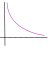
\includegraphics{"./media/ComplexSeries/drawing.png"}
\caption{drawing}
\end{figure}

If I choose some \(\varepsilon\) value, there is always a corresponding
\(\delta\)-value, this \(\delta\)-value will depend on the
\(\varepsilon\)-value:

\begin{figure}
\centering
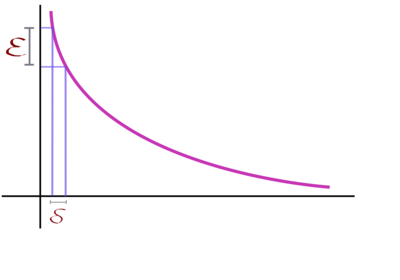
\includegraphics{./media/ComplexSeries/drawing2.png}
\caption{drawing2}
\end{figure}

so the function \(f\left( x \right) = \frac{1}{x}\) is continuous
because: * \(\varepsilon\) can be chosen anywhere * Any \(\varepsilon\)
value will have a corresponding \(\delta\) value.

The function would be uniformly continuous, if: * \(\varepsilon\) can be
chosen anywhere * The Corresponding \(\delta\) value will exist AND not
change size wherever \(\varepsilon\) is chosen.

So in this case the function is not uniformly continuous, because if I
move \(\varepsilon\) down, \(\delta\) would have to get larger, so it IS
NOT uniformly continuous:

\begin{figure}
\centering
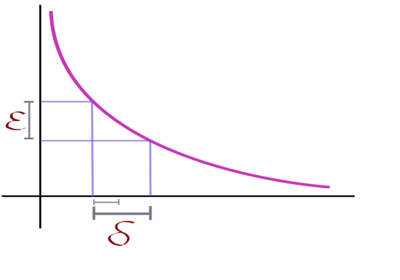
\includegraphics{./media/ComplexSeries/drawing3.png}
\caption{drawing3}
\end{figure}

So basically:

\begin{itemize}
\item
  A function is continuous if a \(\delta\)-value always exists and can
  be described as a function:

  \begin{itemize}
  \item
    \(\delta = \delta\left( \varepsilon, x \right) \)
  \end{itemize}
\item
  A function is uniformly continuous if a \(\delta\)-value always exists
  and can be described as a function only of \(\varepsilon\) :

  \begin{itemize}
  \item
    \(\delta = \delta\left( \varepsilon \right) \)
  \end{itemize}
\end{itemize}

\hypertarget{cantors-theorem}{%
\subsubsection{Cantor's Theorem}\label{cantors-theorem}}

If a function is continuous on an interval \(\left[ a,b \right] \), it
is uniformly continuous on that interval.

\begin{itemize}

\item
  The reasoning being that basically you could chose the smallest
  \(\delta\)-value that will work at all points on that interval
\end{itemize}

\hypertarget{why-is-uniform-continuity-important}{%
\subsubsection{Why is uniform continuity
important?}\label{why-is-uniform-continuity-important}}

Something like,

\begin{itemize}

\item
  if \(f\left( x \right) \) is uniformly continuous
\item
  Then: \[
  \int^{}_{} \lim_{}\left[ f\left( x \right)  \right]   \operatorname{d}x \iff \lim_{}\left[ \int^{}_{} f\left( x \right)   \operatorname{d}x  \right]
  \] but I'm not sure about this so don't quote me, we don't do it here
  so don't worry about it too much, we just need to show that we
  understand it the idea of uniformly continuous functions.
\end{itemize}

\hypertarget{problem-example}{%
\paragraph{Problem Example}\label{problem-example}}

\begin{quote}
Prove that the function \(f\left( x \right) = \frac{1}{1+ x^3}\) is
uniformly continuous on the interval \([1, \infty)\)
\end{quote}

So the first thing to notice is that \emph{Cantor's Theorem} cannot be
applied because it is an open interval.

\textbf{\emph{State the Definition}} \(f\left( x \right)\) is uniformly
convergent if:

\begin{align*}
  \forall x,y \in [1, \infty), \enspace \forall \varepsilon>0,& \enspace \exists \delta\left( \varepsilon \right) :\\
  &0<    \left| x- y \right| <\delta  \implies      \left| f\left( x \right) - f\left( y \right)  \right| < \varepsilon
\end{align*}

 \textbf{\emph{Work Backwards from the \(\varepsilon\) Definition}}

\begin{align*}
  \left| f\left( x \right) - f\left( y \right)  \right| &=     \left| \frac{1}{1+ x^3} - \frac{1}{1+ y^3}\right| \\
  &= \frac{    \left| y^3- x^3 \right| }{    \left| 1+ x^3 \right| \times     \left| 1+ y^3 \right| }\\
  &\leq \frac{    \left| y^3- x^3 \right| }{    \left| 1+ x^3 \right| }\\
  &= \frac{    \left| y- x \right| \cdot     \left| y^2+ xy+ x^2 \right| }{    \left| 1+ x^3 \right| }\\
  \text{Without loss of generality assume that $y<x$}\\
  &\leq     \left| y- x \right| \times 3\cdot \frac{    \left| x^2 \right| }{    \left| 1+ x^3 \right| }\\
  \text{Recall that $x\geq 1  \implies  \frac{1}{    \left| 1+ x^3 \right| }< \frac{1}{    \left| x \right| ^3}$}\\
  &\leq     \left| y- x \right| \cdot \frac{1}{    \left| x \right| } \cdot 3\\
  &\leq     \left| y- x \right| \cdot 3\\
  &\leq     3\cdot \delta\\
\end{align*}

 So choose \(\delta\):
\begin{align*}
3\delta &\leq \varepsilon\\
\delta &\leq \frac{\varepsilon}{3}
\end{align*}

\(\therefore\) it is sufficient to choose
\(\delta\leq \frac{\varepsilon}{3}\).

\textbf{\emph{Proof}}
\begin{align*}
  \forall x,y \in [1,\infty), \enspace \forall \varepsilon>0,& \enspace \exists \delta \leq \frac{\varepsilon}{3}
\end{align*}

\begin{align*}
  \left| x- y \right| < \delta  \implies      \left| f\left( x \right) - f\left( y \right)  \right| &\leq     \left| \frac{1}{1+ x^3} - \frac{1}{1+ y^3} \right| \\
  &\leq     \left| y- x  \right| \cdot \left( \frac{    \left| y^2 \right| +     \left| xy \right| +     \left| x^2 \right| }{    \left| 1+ x^3 \right| \cdot     \left| 1+ y^3 \right| } \right) \\
  &\leq     \left| y- x \right| \cdot \left( \frac{y^2}{    \left| 1+ y^3 \right| } +  \frac{    \left| x \right| \cdot     \left| y \right| }{    \left| 1+ x^3 \right| \cdot 1+ y^3} +  \frac{    \left| x^2 \right| }{    \left| 1+ x^3 \right| } \right) \\
  &leq     \left| y- x \right| \cdot \left( \frac{    \left| y \right| ^2}{    \left| y^3 \right| } +  \frac{    \left| x \right| \cdot     \left| y \right| }{    \left| x \right| ^3\cdot     \left| y \right| ^3} +  \frac{    \left| x \right| ^2}{    \left| x \right| ^3} \right) \\
  &\leq     \left| y- x \right| \cdot \left( \frac{1}{    \left| y \right| } + \frac{1}{    \left| x \right| \cdot     \left| y \right| }+ \frac{1}{    \left| x \right| } \right) \\
  &\leq     \left| y- x \right| \cdot \left(\frac{1}{1}+ \frac{1}{1\times 1}+ \frac{1}{1} \right) \\
  &\leq     \left| y- x \right| \cdot 3\\
  &< 3\cdot \delta\\
  &<3\times \frac{\varepsilon}{3}\\
&<\varepsilon\\
\square
\end{align*}

\end{document}

%\input{11_cauchyIntegrals/drawing.tex}
 %

\iffalse
\documentclass[]{article}
\usepackage{lmodern}
\usepackage{amssymb,amsmath}
\usepackage{ifxetex,ifluatex}
\usepackage{fixltx2e} % provides \textsubscript
\ifnum 0\ifxetex 1\fi\ifluatex 1\fi=0 % if pdftex
  \usepackage[T1]{fontenc}
  \usepackage[utf8]{inputenc}
\else % if luatex or xelatex
  \ifxetex
    \usepackage{mathspec}
  \else
    \usepackage{fontspec}
  \fi
  \defaultfontfeatures{Ligatures=TeX,Scale=MatchLowercase}
\fi
% use upquote if available, for straight quotes in verbatim environments
\IfFileExists{upquote.sty}{\usepackage{upquote}}{}
% use microtype if available
\IfFileExists{microtype.sty}{%
\usepackage[]{microtype}
\UseMicrotypeSet[protrusion]{basicmath} % disable protrusion for tt fonts
}{}
\PassOptionsToPackage{hyphens}{url} % url is loaded by hyperref
\usepackage[unicode=true]{hyperref}
\hypersetup{
            pdfborder={0 0 0},
            breaklinks=true}
\urlstyle{same}  % don't use monospace font for urls
\IfFileExists{parskip.sty}{%
\usepackage{parskip}
}{% else
\setlength{\parindent}{0pt}
\setlength{\parskip}{6pt plus 2pt minus 1pt}
}
\setlength{\emergencystretch}{3em}  % prevent overfull lines
\providecommand{\tightlist}{%
  \setlength{\itemsep}{0pt}\setlength{\parskip}{0pt}}
\setcounter{secnumdepth}{0}
% Redefines (sub)paragraphs to behave more like sections
\ifx\paragraph\undefined\else
\let\oldparagraph\paragraph
\renewcommand{\paragraph}[1]{\oldparagraph{#1}\mbox{}}
\fi
\ifx\subparagraph\undefined\else
\let\oldsubparagraph\subparagraph
\renewcommand{\subparagraph}[1]{\oldsubparagraph{#1}\mbox{}}
\fi

% set default figure placement to htbp
\makeatletter
\def\fps@figure{htbp}
\makeatother


\date{}

\begin{document}

\section{(4) Limits}\label{limits}

\subsection{Limits of Functions
{[}4.1{]}}\label{limits-of-functions-4.1}

Intuitively limits of functions are the expected value of a function at
points that can't be solved because they are undefined, e.g.\\
\hspace*{0.333em}\\
{\$\frac\{(x-2)left( x+2
\right)\}\{left( x-2
\right)\}\$} would be undefined at x=2, however as x is
made sufficiently close to 2, that value will become arbitrarily close
to 4.

\subsubsection{The Limit Generally}\label{the-limit-generally}

From early calculus the limit of {\emph{f}(\emph{x})}, as {\emph{x}}
approaches {\emph{a}} was said to be some value L, denoted
{lim\textsubscript{\emph{x} → \emph{a}}(\emph{f}(\emph{x})) = \emph{L}}\\[2\baselineskip]{$$\begin\{aligned\}
\forall varepsilon \textgreater{} 0,
\enspace, exists delta:
\& \notag  \&
\qquad 0 \textless{} lvert x-a
\rvert \textless{} delta
\implies lvert fleft( x
\right) - L rvert \textless{}
\varepsilon
\label\{stewartlimdef\}end\{aligned\}$$}\\

\subparagraph{Remarks on this
Definition}\label{remarks-on-this-definition}

Observe that the following statements are equivalent:

\begin{enumerate}
\item
  {\$x\neq c enspace
  \wedge enspace lvert
  x-a \rvert \textless{} delta\$}
\item
  {0 \textless{} \textbar{}\emph{x} − \emph{a}\textbar{}\textless{}\emph{δ}}
\item
  {\textbar{}\emph{x} − \emph{a}\textbar{}∈(0,\emph{δ})}
\end{enumerate}

\subparagraph{Notation}\label{notation}

~\\
\hspace*{0.333em}\\
If {\emph{L}} is a limit of {\emph{f}} at {\emph{c}}, then it is said
that:

\begin{enumerate}
\item
  {\emph{f}} converges to {\emph{L}} at {\emph{c}}
\item
  {\emph{f}(\emph{x})} approaches {\emph{L}} as {\emph{x}} approaches
  {\emph{c}} This is sometimes expressed with the symbolism
  {\emph{f}(\emph{x}) → \emph{L}} as {\emph{x} → \emph{c}}
\end{enumerate}

~\\
And the following notation is used

\begin{enumerate}
\item
  {lim\textsubscript{\emph{x} → \emph{c}}(\emph{f}(\emph{x})) = \emph{L}}
\item
  {lim\textsubscript{\emph{x} → \emph{c}}\emph{f}}
\end{enumerate}

\subsubsection{The Limit Using Cluster
Points}\label{the-limit-using-cluster-points}

In analysis we more or less use the same definition but we introduce the
concept of cluster points to make it more rigorous.

\subparagraph{Neighborhoods {[}2.2.7{]}}\label{neighborhoods-2.2.7}

A neighborhood is an interval about a value, e.g. the
{\emph{ε}}-neighborhood of {\emph{a}} is some set
{\emph{V}\textsubscript{\emph{ε}}(\emph{a})}:\\
{$$\begin\{aligned\}
V\_\{\varepsilon\}(a) = left(
\varepsilon-a, varepsilon+a
\right) \&= left\{ x :
\varepsilon - a \textless{} x \textless{}
\varepsilon + a right\}
\ \&=
\left\{ x : -varepsilon
\textless{} x - a \textless{} \varepsilon
\right\}
\&= \left\{ x: lvert x-a
\rvert \textless{} varepsilon
\right\}
\label\{nebhdef\}end\{aligned\}$$}\\

\subparagraph{Cluster Points}\label{cluster-points}

Let {\emph{c}} be a real number and let {\emph{A}} be a subset of the
real numbers, {\emph{c}} may or may not be contained by {\emph{A}} it
doesn't matter.\\
Take some interval around {\emph{c}}, or rather consider the
{\emph{ε}}-neighborhood of {\emph{c}},\\
if, some value (other than {\emph{c}}) can be found inside that
interval/neighborhood that is also inside {\emph{A}}, regardless of how
small that interval is made, Then {\emph{c}} is said to be a cluster
point of {\emph{A}}.\\
\hspace*{0.333em}\\
i.e., if the following is true\\
{\$\forall varepsilon \textgreater{} 0,
\enspace exists xneq c
\in Acap
V\_\{\varepsilon\}(c)\$}\\
then {\emph{c}} is said to be a cluster point of {\emph{A}}.\\
\hspace*{0.333em}\\
It basically means that there are infinitely infinitesimal points
between any point in {\emph{A}} and the value {\emph{c}}.

Example

\begin{itemize}
\item
  The point {4} of the set {\{3,4,5\}} is not a cluster point of that
  set because a 0.1-neighbourhood of 4 would be the set
  {\emph{V}\textsubscript{0.1}(4)=\{4\}}, this set does not contain a
  value {\emph{x} ≠ 4} that is also inside the original set.\\
\item
  The point 6 of {(1,6) = \{\emph{x}:1\textless{}\emph{x}\textless{}6\}}
  is a cluster point of {(1,6)} because no matter how small a
  neighborhood is made around 6, there will always be values
  {\emph{x} ≠ 6} inside that interval that are also inside {(1,6)} also
  observe that in this case {6 ∉ (1,6)}
\end{itemize}

\subparagraph{Definition of the Limit
{[}4.1.4{]}}\label{definition-of-the-limit-4.1.4}

So this is the definition that we moreso use in this unit and the one to
memorise (or the Neighborhoods one seems simpler to memorise).\\
\hspace*{0.333em}\\
Let {\emph{A} ⊆ ℝ} and let {\emph{c}} be a cluster point of
{\emph{A}}.\\
\hspace*{0.333em}\\
Now take some function:\\
{$$\begin\{aligned\} f: A rightarrow
\mathbb\{R\} label\{clustlimdeffunc\}
\end\{aligned\}$$}\\
It is said that {\emph{L}} is a limit of {\emph{f}} at {\emph{c}} if:\\
{$$\begin\{aligned\} forall
\varepsilon \textgreater{} 0, \&enspace
\exists delta \textgreater{} 0:
\notag
\qquad \& left( x in A
\enspace wedge enspace
0\textless{}\lvert x-c rvert \textless{}
\delta right) implies
\lvert fleft( x right) -
L \rvert \textless{} varepsilon
\tag\{4.1.4\} label\{414\}
\end\{aligned\}$$}\\

What's the Distinction

This is more or less the same as the typical definition given in early
calculus ({[}stewartlimdef{]}), the distinction here is that we have
specified that {\emph{c}} must be a cluster point of {\emph{A}}, this is
more rigorous because c is always such that there are infinitely many
values in any infinitesimal distance between intself and any
{\emph{x} ∈ \emph{A}},\\
So the limit will always mean a continuous approach as we expect, this
is just a more thorough definition.

\subparagraph{Definition using Neigborhoods
{[}4.1.6{]}}\label{definition-using-neigborhoods-4.1.6}

A value {\emph{L}} is said to be the limit of {\emph{f}} as
{\emph{x} → \emph{c}}, denoted
{lim\textsubscript{\emph{x} → \emph{c}}(\emph{f}(\emph{x}))} if and only
if:\\

{2em}{0pt} \emph{For any} given {\emph{ε}}-neighbourhood of {\emph{L}},
{\$\enspace V\_\{varepsilon\}(L)\$}\\
\emph{There exists} a {\emph{δ}}-neighbourhood of {\emph{c}},
{\$\enspace
V\_\{\delta\}left( L
\right)\$}\\

such that: ~\\

{4em}{0pt} =0.7cm \emph{If} {\emph{x} ≠ \emph{c}} is in both {\emph{A}}
and {\emph{V}\textsubscript{\emph{δ}}(\emph{c})}\\
=0.5cm \emph{Then} {\emph{f}(\emph{x})} must be within the neighbourhood
{\emph{V}\textsubscript{\emph{ε}}(\emph{L})}

Formally

{$$\begin\{aligned\} forall
\varepsilon \textgreater{} 0, \& enspace
\exists delta \textgreater{} 0:
\notag  \&
\qquad x neq c, enspace x
\in Acap
V\_\{\varepsilon\}left( L
\right) implies fleft( x
\right) in
V\_\{\delta\}left( c
\right) tag\{4.1.6\}
\label\{416\}end\{aligned\}$$}\\

Defintions ({[}416{]}) and ({[}414{]}) are equivalent, and are both
consistent with the initial less rigorous definition
({[}stewartlimdef{]}).

\subparagraph{Only one Limit Value
{[}4.1.5{]}}\label{only-one-limit-value-4.1.5}

If {\emph{f} : \emph{A} → ℝ} and {\emph{c}} is a cluster point of
{\emph{A}}, then there is only one value L:
{lim\textsubscript{\emph{x} → \emph{c}}(\emph{f}(\emph{x})) = \emph{L}}

\subsubsection{Using Sequences to Define Limits {[} 4.1.8
{]}}\label{using-sequences-to-define-limits-4.1.8}

Now that limits are defined we can use sequences to define them as well,
this will give us more tools to use later and allows a connection to be
made between material of Chapter 3 and 4.

\subparagraph{Definition}\label{definition}

A value {\emph{L}} is said to be the limit of {\emph{f}} as
{\emph{x} → \emph{c}}, denoted
{lim\textsubscript{\emph{x} → \emph{c}}(\emph{f}(\emph{x}))} if and only
if:\\

{2em}{0pt} \emph{For every} sequence
{(\emph{x}\textsubscript{\emph{n}})} in {\emph{A}},\\

{4em}{0pt} \emph{if} {(\emph{x}\textsubscript{\emph{n}})} converges to
{\emph{c}} such that {\emph{x}\textsubscript{\emph{n}} ≠ \emph{c}},\\

{4em}{0pt} \emph{Then} {(\emph{f}(\emph{x}\textsubscript{\emph{n}}))}
converges to {\emph{L}}

~\\
So basically, again, if {\emph{x}} gets close to {\emph{c}},
{\emph{f}(\emph{x})} gets close to L, but we took {\emph{x}} from a
sequence.

\subsubsection{Divergence Criteria {[} 4.1.9
{]}}\label{divergence-criteria-4.1.9}

Now we can use the \emph{Divergence Criteria} from {[}3.4.5{]} to
determine whether or not a limit exists generally or at a point.

\subparagraph{(a) Limit is not a Specific
Value}\label{a-limit-is-not-a-specific-value}

If {\emph{L} ∈ ℝ}, then {\emph{f}} does not have a limit at {\emph{c}},
if and only if:\\
\hspace*{0.333em}\\
There is a sequence {(\emph{x}\textsubscript{\emph{n}})} in {\emph{A}}
with {\emph{x}\textsubscript{\emph{n}} ≠ \emph{c}}, such that:\\
{(\emph{x}\textsubscript{\emph{n}})} converges to {\emph{c}} but the
sequence {\emph{f}(\emph{x}\textsubscript{\emph{n}})} does not converge
to {\emph{L}}

\subparagraph{(b) No Limit whatsover}\label{b-no-limit-whatsover}

If {\emph{L} ∈ ℝ}, then {\emph{f}} does not have a limit at {\emph{c}},
if and only if:\\
\hspace*{0.333em}\\
There is a sequence {(\emph{x}\textsubscript{\emph{n}})} in {\emph{A}}
with {\emph{x}\textsubscript{\emph{n}} ≠ \emph{c}}, such that:\\
{(\emph{x}\textsubscript{\emph{n}})} converges to {\emph{c}} but the
sequence {\emph{f}(\emph{x}\textsubscript{\emph{n}})} does not converge
in {ℝ}

\subparagraph{The Signum Function}\label{the-signum-function}

The Signum function returns the sign of the input value:

{$$\begin\{aligned\} sgnleft( x
\right) \&:= begin\{cases\} +\&1
\qquad text\{for\}
\enspace \$x textgreater
\enspace 0\$  \&0
\qquad text\{for\}
\enspace \$x= 0\$  -\&1
\qquad text\{for\}
\enspace \$x textless
\enspace 0\$ end\{cases\}
\tag\{4.1.10\} label\{4110\}
\ \&=
\frac\{x\}\{lvert x
\rvert\}
\notagend\{aligned\}$$}\\

\subsection{Limit Theorems {[}4.2{]}}\label{limit-theorems-4.2}

These are useful for calculating limits of functions, they are mostly
extensions of {[}3.2{]}.

\subsubsection{Bounded Functions}\label{bounded-functions}

\subparagraph{Definition}\label{definition-1}

Let {\emph{A} ⊆ ℝ}, {\emph{f} : \emph{A} → ℝ} and let {\emph{c} ∈ ℝ} be
a cluster point of {\emph{A}}.\\
It is said that \emph{f is bounded on a neighbourhood of} {\emph{c}}
if:\\

{2em}{0pt} there exists a {\emph{δ}}-neighborhood
{\emph{V}\textsubscript{\emph{δ}}(\emph{c})} and some constant value
{\emph{M} \textgreater{} 0} such that:\\

{4em}{0pt} {\textbar{}\emph{f}(\emph{x})\textbar{}≤\emph{M}} for every
{\emph{x} ∈ \emph{A} ∩ \emph{V}\textsubscript{\emph{δ}}(\emph{c})}

~\\
So basically a function is said to be \emph{bounded on a neighbourhood
of {\emph{c}}} if:

{4em}{0pt} for some interval (It doesn't matter how small) around
{\emph{c}},

{6em}{0pt} {\emph{f}(\emph{x})} can be contained in some interval

~\\

{4em}{0pt} {\$\exists
\delta\textgreater{}0, enspace
\exists M\textgreater{}0:\$}

{6em}{0pt}
{\emph{x} ∈ \emph{V}\textsubscript{\emph{δ}}(\emph{c}) ⟹ \textbar{}\emph{f}(\emph{x})\textbar{}\textless{}\emph{M}}

~\\
So for example:

\begin{itemize}
\item
  {\emph{f}(\emph{x}) = \emph{x}\textsuperscript{3}} is \emph{bounded on
  every neighborhood of every {\emph{x} ∈ ℝ}} whereas,
\item
  {\$g\left( x right) =
  \sfrac\{1\}\{x\}\$} is \emph{\textbf{not} bounded on a
  neighborhood of 0} because {\emph{g}(\emph{x})} tends to infinity as
  {\emph{x} → 0},

  \begin{itemize}
  \item
    {furthermore {\emph{g}(\emph{x})} is \emph{bounded on \textbf{some
    but notall} neighborhoods of 1}, because an interval around 1 must
    not be drawn large enough to encapsulate 0.}
  \end{itemize}
\end{itemize}

\subparagraph{Limits imply Bounded Neighbourhoods {[}4.2.2
{]}}\label{limits-imply-bounded-neighbourhoods-4.2.2}

A function is bounded on a neighborhood of a point that is a limit of
that function.\\
If a function has a limit at {\emph{c}}, then {\emph{f}} must be
\emph{bounded on some neighborhood of {\emph{c}}},\\
this flows from the initial definitions because we know that {\emph{c}}
is a cluster point and that {(\emph{f}(\emph{x}))} moves closer to
{\emph{L}},\\
hence it must be possible to draw a small enough interval (e.g.
horizontal lines on the {\emph{y}}-axis) to contain all
{\emph{f}(\emph{x})} defined by

\subsubsection{Functions and Arithmetic
{[}4.2.3{]}}\label{functions-and-arithmetic-4.2.3}

Just like with sequences we can define arithmetic operations that relate
to addition and multiplication with functions in order to manipulate
them:\\
\hspace*{0.333em}\\
Let {\emph{A} ⊆ ℝ} ,\\
{$$\begin\{aligned\} f: A rightarrow
\mathbb\{R\} qquad g: A
\rightarrow mathbb\{R\}
\qquad h: A rightarrow
\mathbb\{R\}, enspace h(x)
\neq 0, enspace forall x
\in A
\label\{seqdefgen\}end\{aligned\}$$}\\

We define the following Operations {[}4.2, p. 111{]}:

{$$\begin\{aligned\} \{1\} left( f+g
\right) left( x right)
\&:= f\left( x right) +
g\left( x right)
\label\{addfundef\}
\left( f-g right) left( x
\right) \&:= fleft( x
\right) + gleft( x right)
\label\{subfundef\}
\left( fg right) left( x
\right) \&:= fleft( x
\right) times gleft( x
\right) label\{multfundef\}
\ left( bf
\right) left( x right)
\&:= b \times fleft( x
\right) label\{confundef\}
\ left(
\frac\{f\}\{h\}
\right)left( x right)
\&:= \frac\{fleft( x
\right)\}\{hleft( x
\right)\} end\{aligned\}$$}\\

Limits of Function Operations {[}4.2.4{]}

Because the limit of a function is essentially the expected value of the
function around that value, it stands to reason that the limit will
distribute over the basic operations:\\
{Let the functions be defined as they were in ({[}seqdefgen{]}) and let
{\emph{c} ∈ ℝ} be a custer point of {\emph{A}}.}

{$$\begin\{aligned\} lim\_\{x
\rightarrow c\}left( f
\right) = L qquad
\lim\_\{x rightarrow
c\}\left( g right) = M
\quad lim\_\{xrightarrow
c\}\left( h right) = H
\neq 0
\label\{fundeflim\}end\{aligned\}$$}\\

Then the limits are:

{$$\begin\{aligned\} \{2\}
\lim\_\{xrightarrow c\}
\left( f+g right) \&=
\lim\_\{xrightarrow
c\}\left( f right) +
\lim\_\{xrightarrow
c\}\left( g right) \&= L + M
\label\{addlimdef\}
\{[}1em{]}
\lim\_\{xrightarrow c\}
\left( f-g right) \&=
\lim\_\{xrightarrow c\}
\left( f right) -
\lim\_\{xrightarrow c\}
\left( g right) \&= x - y
\label\{minlimdef\}
\{[}1em{]}
\lim\_\{xrightarrow c\}
\left( c cdot f right)
\&= c \cdot
\lim\_\{xrightarrow c\}
\left( f right) \&= c
\cdot x label\{conmultlimdef\}
\{[}1em{]}
\lim\_\{xrightarrow c\}
\left( ftimes g right)
\&= \lim\_\{xrightarrow c\}
\left( f right) times
\lim\_\{xrightarrow c\}
\left( g right) \&= x
\times y label\{multlimdef\}
\{[}1em{]}
\lim\_\{xrightarrow c\}
\left( f/h right) \&=
\lim\_\{xrightarrow c\}
\left( f right) div
\lim\_\{xrightarrow c\}
\left( h right) \&=
\sfrac\{x\}\{y\}
\label\{divlimdef\}end\{aligned\}$$}\\

\subsubsection{Limit Theorems}\label{limit-theorems}

The rest of the chapter just provides values of varios limits.\\
{Let the functions be defined as they were in ({[}seqdefgen{]}) and let
{\emph{c} ∈ ℝ} be a custer point of {\emph{A}}.}

\subparagraph{Limits Captured in Intervals
{[}4.2.6{]}}\label{limits-captured-in-intervals-4.2.6}

~\\
\hspace*{0.333em}\\
\emph{if} {\emph{f}(\emph{x}) ∈ {[}\emph{a},\emph{b}{]}} for all {\$x
\in A, enspace x neq
c\$}, and {lim\textsubscript{\emph{x} → \emph{c}}(\emph{f})} exists,\\

{2em}{0pt} \emph{then} {\emph{f}(\emph{x}) ∈ {[}\emph{a},\emph{b}{]}}

\subparagraph{Squeeze Theorem {[}4.2.7{]}}\label{squeeze-theorem-4.2.7}

if {[}4.2.6{]} is extended to functions, then we have the squeeze
theorem:\\
\emph{if} {\emph{g}} is within an interval defined by the functions
{\emph{f}} and {\emph{h}}:

{$$\begin\{aligned\} fleft( x
\right) leq gleft( x
\right) leq hleft( x
\right), quad forall
x\in A, enspace xneq c
\label\{squeezelimdist\}end\{aligned\}$$}\\

{2em}{0pt} \emph{then} the limit of g must also be 0

{$$\begin\{aligned\}
\lim\_\{xrightarrow
c\}\left( g right)=L
\label\{limisL\}end\{aligned\}$$}\\

\subparagraph{A Positive Limit implies a neighbourhood with Positive
Values}\label{a-positive-limit-implies-a-neighbourhood-with-positive-values}

Let {\emph{A} ⊆ ℝ} and let {\emph{c} ∈ ℝ} be a cluster point of
{\emph{A}} as in (3.4.6) above.\\
\emph{If}:\\
{$$\begin\{aligned\}
\lim\_\{xrightarrow
c\}\left( f right) \textgreater{} 0
\label\{limneighbourpor\}end\{aligned\}$$}\\

\emph{Then:}

{4em}{0pt} there is a neighborhood
{\emph{V}\textsubscript{\emph{δ}}(\emph{c})} such that
{\$f\left( x right) \textgreater{}0,
\enspace forall x in A
\cap V\_\{delta\}left( c
\right)\$}

~\\
This also holds for negative values and basically all it says, in more
rigorous language, is that if the limit point is above the
{\emph{x}}-axis then there's gotta be points to the left and right that
are above the {\emph{x}}-axis as well (because the whole cluster point
thing means everything can be arbitrarily small).\\
\hspace*{0.333em}\\
Although this may start to seem a little pointless, the idea of making
the definitions this rigorous is like writing code in a scripting
language, by using this very precise language, the logical consequences
give us exactly the concept that we want, even though we need to take a
longer or alternate path to get to that concept than we would otherwise
would generally take in order to describe the concept.

\subsection{Extensions of the Limit Concept
{[}4.3{]}}\label{extensions-of-the-limit-concept-4.3}

These are written in a particularly convoluted fashion, however if the
preceeding material is understood the textbook can be used more or less
as a reference, hence these notes will be brief.

\subsubsection{One-Sided Limits
{[}4.3.1{]}}\label{one-sided-limits-4.3.1}

\subparagraph{Definition {[}4.3.1{]}}\label{definition-4.3.1}

Let {\emph{c} ∈ ℝ} be a cluster point of {\$A\cap
\left( c, infty right) =
\left\{ x in A
\enspace : enspace x \textgreater{} c
\right\}\$}\\
It is said that {\emph{L}} is a \emph{Right-hand limit of {\emph{f}} at
{\emph{c}}} and it is written:\\
{$$\begin\{aligned\} lim\_\{x
\rightarrow c\^{}+\} left( f
\right) = L tag\{4.3.1\}
\label\{431\}end\{aligned\}$$}\\

This can be extended to left-hand limits as well.

Definition in Term of Sequences {[}4.3.2{]}

As above it is said that {\emph{L}} is a \emph{Right-hand limit of
{\emph{f}} at {\emph{c}}} if:

{2em}{0pt} Every sequence {(\emph{x}\textsubscript{\emph{n}})} in
{\emph{A}} that converges to {\emph{c}} is such that
{\emph{f}(\emph{x}\textsubscript{\emph{n}})} converges to {\emph{L}},
given that {\$x\_n\textgreater{}c, \enspace
\forall n in
\mathbb\{N\}\$}

\subparagraph{Limit must be equal on both
sides}\label{limit-must-be-equal-on-both-sides}

A limit is defined only if the limit is equal from both directions\\
{$$\begin\{aligned\}
\lim\_\{xrightarrow
c\}\left( f right) = L
\iff lim\_\{xrightarrow
c\^{}+\}\left( f right) = L =
\lim\_\{xrightarrow c
\}\left( f right)
\tag\{3.4.3\}
\label\{343\}end\{aligned\}$$}\\

\subsubsection{Infinite Limits {[}4.3.5{]}}\label{infinite-limits-4.3.5}

Let {\emph{c} ∈ ℝ} be a cluster point of {\emph{A}},\\
It is aid that {\emph{f}} tends to {∞} as {\emph{x} → \emph{c}}, and it
is written:

{$$\begin\{aligned\}
\lim\_\{xrightarrow
c\}\left( f right) =
\infty tag\{4.3.5\}
\label\{435\}end\{aligned\}$$}\\

If {∀\emph{α} ∈ ℝ}, {\$\enspace exists
\delta \textgreater{} 0\$}:

{6em}{0pt}
{0 \textless{} \textbar{}\emph{x} − \emph{c}\textbar{}\textless{}\emph{δ} ⟹ \emph{f}(\emph{x})\textgreater{}\emph{α},  ∀\emph{x} ∈ \emph{A}}

\subparagraph{One-Sided Limits to Infinity
{[}4.3.8{]}}\label{one-sided-limits-to-infinity-4.3.8}

Let {\emph{c} ∈ ℝ} be a cluster point of {\$A\cap
\left( c, infty right) =
\left\{ x in A
\enspace : enspace x \textgreater{} c
\right\}\$},\\
It is aid that {\emph{f}} tends to {∞} as
{\emph{x} → \emph{c}\textsuperscript{+}}, and it is written:

{$$\begin\{aligned\}
\lim\_\{xrightarrow
c\}\left( f right) =
\infty tag\{4.3.8\}
\label\{438\}end\{aligned\}$$}\\

If {∀\emph{α} ∈ ℝ}, {\$\enspace exists
\delta \textgreater{} 0\$}:

{6em}{0pt}
{0 \textless{} \emph{x} − \emph{c} \textless{} \emph{δ} ⟹ \emph{f}(\emph{x})\textgreater{}\emph{α},  ∀\emph{x} ∈ \emph{A}}

\subparagraph{Ordered Functions}\label{ordered-functions}

If {\emph{f}(\emph{x}) \textless{} \emph{g}(\emph{x})}, then:\\
{$$\begin\{aligned\}
\lim\_\{xrightarrow
c\}\left( f right) =
\infty \&implies lim\_\{x
\rightarrow c\}left( g
\right) = infty
\tag\{4.3.7 (a)\}
\label\{437a\}
\lim\_\{xrightarrow
c\}\left( g right) =
-\infty \&implies
\lim\_\{x rightarrow
c\}\left( f right) =
-\infty tag\{4.3.7 (b)\}
\label\{437b\}end\{aligned\}$$}\\

\subsubsection{Limits at Infinity
{[}4.3.10{]}}\label{limits-at-infinity-4.3.10}

It is also useful to talk about limits as {\emph{x}} tends to {∞}

Let {(\emph{a},∞) ⊆ \emph{A} ⊆ ℝ} for some {\emph{ain}ℝ}\\
It is aid that the limit of {\emph{f}} as {\emph{x} → ∞} is {\emph{L}},
and it is written:\\
{$$\begin\{aligned\}
\lim\_\{xrightarrow
\infty\}left( f right) =
L \tag\{4.3.10\}
\label\{4310\}end\{aligned\}$$}\\

If {\$ \forall varepsilon
\textgreater{}0, \enspace exists K
\textgreater{} 0\$}:

{6em}{0pt}
{\emph{x} \textgreater{} \emph{K} ⟹ \textbar{}\emph{f}(\emph{x}) − \emph{L}\textbar{}\textless{}\emph{ε}}

Limits at Infinity in Terms of Sequences {[}4.3.11{]}

equivalently to ({[}4310{]}), the definition can be expressed in terms
of sequences:\\

{2em}{0pt} Every sequence {(\emph{x}\textsubscript{\emph{n}})} in
{\emph{A} ∩ (\emph{a},∞)} that has
{lim(\emph{x}\textsubscript{\emph{n}})=∞} is such that the sequence
{(\emph{f}(\emph{x}\textsubscript{\emph{n}}))} converges to {\emph{L}}

\subparagraph{Infinite Limits at
Infinity}\label{infinite-limits-at-infinity}

So this basically combines {[}4.3.10{]} with {[}4.3.5{]}

Let {(\emph{a},∞) ⊆ \emph{A} ⊆ ℝ} for some {\emph{a} ∈ ℝ}\\
\hspace*{0.333em}\\
It is aid that {\emph{f}} tends to {∞} as {\emph{x} → ∞}, and it is
written:\\
{$$\begin\{aligned\}
\lim\_\{xrightarrow
\infty\}left( f right) =
\infty tag\{4.3.13\}
\label\{4313\}end\{aligned\}$$}\\

If {\$ \forall varepsilon
\textgreater{}0, \enspace exists K
\textgreater{} \alpha\$}:

{6em}{0pt}
{\emph{x} \textgreater{} \emph{K} ⟹ \emph{f}(\emph{x}) \textgreater{} \emph{α}}

Infinite Limits at Infinity in Terms of Sequences {[}4.3.14{]}

equivalently to ({[}4313{]}), the definition can be expressed in terms
of sequences:\\

{2em}{0pt} Every sequence {(\emph{x}\textsubscript{\emph{n}})} in
{\emph{A} ∩ (\emph{a},∞)} that has
{lim(\emph{x}\textsubscript{\emph{n}})=∞} is such that the limit of the
sequence of function values
{lim (\emph{f}(\emph{x}\textsubscript{\emph{n}})) = ∞}

Ratios of Functions

This result uses (4.3.14) to restate (3.6.5) in terms of functions:\\
If {\$g\left( x right) \textgreater{} 0
\enspace forall x \textgreater{} a\$} and
{\emph{L} ≠ 0} is defined:

{$$\begin\{aligned\} lim\_\{xrightarrow
\infty\}left(
\frac\{fleft( x
\right)\}\{gleft( x
\right)\} right)
\tag\{4.3.15\}
\label\{4315\}end\{aligned\}$$}\\

then,

{$$\begin\{aligned\} L \textgreater{} 0
\implies
\lim\_\{xrightarrow
\infty\}left( f right) =
\infty iff lim\_\{x
\rightarrow infty left( g
\right) = infty\}
\tag\{4.3.15 (i)\} label\{4315i\}
\ L \textless{} 0 implies
\lim\_\{xrightarrow
\infty\}left( f right) =
- \infty iff lim\_\{x
\rightarrow infty left( g
\right) = infty\}
\tag\{4.3.15 (ii)\}
\label\{4315ii\}end\{aligned\}$$}\\

\end{document}

\fi

 %
 %\documentclass[class=article, crop=false]{standalone}


%%%%%%%%%%%%%%%%%%%%%%%%%%%%%%
%%%%%%%%Preamble%%%%%%%%%%%%%%
%%%%%%%%%%%%%%%%%%%%%%%%%%%%%%

%Packages ------------------------------------

\usepackage{amsmath, amssymb, amsthm}
\usepackage[utf8]{inputenc}
%\usepackage[framemethod=tikz]{mdframed}
\usepackage{pgfplots}
\usepackage{tikz, pstricks}
\usepackage{graphicx}
%\usetikzlibrary{calc}
%\usepackage{chngcntr}
\usepackage[T1]{fontenc}
\usepackage{extsizes} % More Font Sizes
\usepackage[utf8]{inputenc}
\usepackage{amsmath}
\usepackage{sectsty} %Need it for underlining Sections
\usepackage{listings}
\usepackage{lmodern}
\usepackage{amssymb,amsmath}
\usepackage{enumitem}
\usepackage{ifxetex,ifluatex}
\usepackage{lipsum}
\usepackage[T1]{fontenc}
\usepackage[utf8]{inputenc}
\usepackage[margin=1in]{geometry}
\addtolength{\skip\footins}{2pc plus 5pt} %Add whitespace before footnotes`
%\usepackage[svgnames, x11names, dvipsnames]{xcolor} %This is included with mdframed
%\usepackage{tgadventor}
%\usepackage{titlesec} % Section Colours




%Hyperlinks-----------------------------------
\usepackage{hyperref}
\hypersetup{
	colorlinks,
	citecolor=black,
	filecolor=black,
	linkcolor=black,
	urlcolor=black,
	 colorlinks=true, %set true if you want colored links
	linktoc=all     %set to all if you want both sections and subsections linked
}

%Remove Section Numbers----------------
\makeatletter
\renewcommand{\@seccntformat}[1]{}
\makeatother

%Change the Font------------------------------
%\usepackage{PoiretOne}
\renewcommand*\familydefault{\sfdefault} %% Only if the base font of the document is to be sans serif

% Add rule after sections ------------------------------
\usepackage{titlesec}


%Listings----------------------------------------


\definecolor{dkgreen}{rgb}{0,0.6,0}
\definecolor{gray}{rgb}{0.5,0.5,0.5}
\definecolor{mauve}{rgb}{0.58,0,0.82}
\lstset{
%  frame=tb,
  frame=leftline,
  framesep=15pt,
  language=Java,
  aboveskip=15pt,
  belowskip=20pt,
  showstringspaces=false,
  columns=flexible,
  basicstyle={\small\ttfamily},
  numbers=none,
%  backgroundcolor=\color{Snow2},
  numberstyle=\tiny\color{gray},
  keywordstyle=\color{blue},
  commentstyle=\color{dkgreen},
  stringstyle=\color{mauve},
  breaklines=true,
  breakatwhitespace=true,
  tabsize=3,
  xleftmargin=1in,
}

	% Formatting----------------------------------------
	\widowpenalty=1000
	\clubpenalty=1000

% Problem boxes --------------------------------------

%\newtheorem*{prob}{Problem}
%\theoremstyle{working}{\cmss}
%\newtheorem*{working}{Worked Solution}
\renewcommand{\qedsymbol}{$\blacksquare$}


\newenvironment{prob}[1][Problem]{%
	\sffamily \itshape   %
}{\endproof} %\itshape for italics

\newenvironment{sol}[1][Problem]{%
	\proof[\nopunct]  %
}{\endproof}

%\renewenvironment{proof}{{\bfseries \fontfamily{ccr} \selectfont Proof}}{*something*}



%%%%%%%%%%%%%%%%%%%%%%%%%%%%%%%%%%%%%%%%%%%%%
%%%%%%Heading Colurs and Format%%%%%%%%%%%%%%
%%%%%%%%%%%%%%%%%%%%%%%%%%%%%%%%%%%%%%%%%%%%%
% Numbering
\renewcommand{\thesection}{}
\renewcommand{\thesubsection}{}


%%%% Define Heading colours
\definecolor{colsse}{RGB}{136, 73, 143}
\definecolor{colsss}{RGB}{156, 118, 160}
\definecolor{colspg}{RGB}{218, 168, 224}
\definecolor{coltit}{RGB}{84, 65, 86}
\definecolor{colname}{RGB}{236, 66 ,255}
		
	
	
% Change Section Colour
\titleformat{\section}
{\color{colsse}\normalfont\LARGE\bfseries}
{\color{colsse}\thesection}{-1em}{}
\fontfamily{cmss}\selectfont

%SubSection
\titleformat{\subsection}
{\color{colsss}\normalfont\Large\bfseries}
{\color{colsss}\thesubsection}{-1em}{}[\rule{4 in}{2pt}]
\fontfamily{cmss}\selectfont
% Change Font
\fontfamily{cmss}\selectfont



%Paragraph
\titleformat{\paragraph}
{\color{colsss}\normalfont\large}
{\color{colsss}\theparagraph}{9em}{}[\rule{2 in}{1 pt}]
\fontfamily{cmss}\selectfont
% Change Font
\fontfamily{cmss}\selectfont


%%%%%%%Title
\title{\color{coltit} \Huge Squared Partial Derivative}
\author{Ryan Greenup ; 1780-5315}





%%%%%%%%%%%%%%%%%%%%%%%%%%%%%%
%%%%%%Document%%%%%%%%%%%%%%%%
%%%%%%%%%%%%%%%%%%%%%%% %%%%%%%
\begin{document}

\maketitle
\tableofcontents

If:
$$
u\left( x,y \right)= F\left( \frac{y}{x} \right)+ G\left( \frac{y}{x} \right)
$$
Show that:

$$
x^2 \frac{\partial^2 u }{\partial x^2 } +  2xy \cdot  \frac{\partial^2 u }{\partial x \partial y} +  y^2 \frac{\partial^2 u }{\partial y^2} = 0
$$

\section{Solve the Partial Derivatives}

\begin{lstlisting}[language = Mathematica]
D[u[x, y], {x, 2}]
D[D[u[x, y], x], y]
D[D[u[x, y], y], x]
D[u[x, y], {y, 2}]
\end{lstlisting}	

This gives:

$$
\begin{aligned}
  \frac{\partial^2 u }{\partial x^2} &= \frac{y^2 F''\left(\frac{y}{x}\right)}{x^4}+\frac{2 y F'\left(\frac{y}{x}\right)}{x^3}+\frac{y^2 G''\left(\frac{y}{x}\right)}{x^4}+\frac{2 y G'\left(\frac{y}{x}\right)}{x^3} \\
  \frac{\partial^2 u }{\partial xy} &= -\frac{y F''\left(\frac{y}{x}\right)}{x^3}-\frac{F'\left(\frac{y}{x}\right)}{x^2}-\frac{y G''\left(\frac{y}{x}\right)}{x^3}-\frac{G'\left(\frac{y}{x}\right)}{x^2}\\
  \frac{\partial^2 u }{\partial yx}&= -\frac{y F''\left(\frac{y}{x}\right)}{x^3}-\frac{F'\left(\frac{y}{x}\right)}{x^2}-\frac{y G''\left(\frac{y}{x}\right)}{x^3}-\frac{G'\left(\frac{y}{x}\right)}{x^2} \\
  \frac{\partial^2 u }{\partial y^2} &=  \frac{F''\left(\frac{y}{x}\right)}{x^2}+\frac{G''\left(\frac{y}{x}\right)}{x^2}
\end{aligned}
$$
So clearly where $x \neq 0$ the mixed partials will be equal given that $F$ and $G$ are continuous. \\

Now multiplying through by $x^2$, $2xy$ and $y^2$ respectively:

\begin{lstlisting}[language = Mathematica]
Simplify[(D[u[x, y], {x, 2}] * x^2  )]
Simplify[D[D[u[x, y], x], y] * 2*x*y]
Simplify[D[u[x, y], {y, 2}] * y^2]
\end{lstlisting}	

Which gives:

$$
\begin{aligned}
x^2 \frac{\partial^2 u }{\partial x^2} &= \frac{y \left(y \left(F''\left(\frac{y}{x}\right)+G''\left(\frac{y}{x}\right)\right)+2 x F'\left(\frac{y}{x}\right)+2 x G'\left(\frac{y}{x}\right)\right)}{x^2} \\
2xy \frac{\partial^2 u }{\partial xy} = 2xy \frac{\partial^2 u }{\partial yx} &=   -\frac{2 y \left(y \left(F''\left(\frac{y}{x}\right)+G''\left(\frac{y}{x}\right)\right)+x F'\left(\frac{y}{x}\right)+x G'\left(\frac{y}{x}\right)\right)}{x^2}\\
y^2 \frac{\partial^2 u }{\partial y^2} &= \frac{y^2 \left(F''\left(\frac{y}{x}\right)+G''\left(\frac{y}{x}\right)\right)}{x^2}
\end{aligned}
$$
Summing these terms: 

\begin{lstlisting}[language = Mathematica]
FullSimplify[Simplify[(D[u[x, y], {x, 2}] * x^2  )] +
  Simplify[D[D[u[x, y], x], y] * 2*x*y] +
  Simplify[D[u[x, y], {y, 2}] * y^2]]
\end{lstlisting}	

Gives $0$, so clearly the identity is valid and all the terms will cancel out, it's just a function of showing it.








 
\end{document}















 %\input{classnotes/classnotes.tex}


\part{Tutorial Workings}

%\input{T1Q3.4/tut1abs 2019-03-09 10_25_13.tex}

\part{Assessment Material}
\begin{appendix}
  \listoftables
  \listoffigures
\end{appendix}

\end{document}

%% TODO Titles
    %% TODO Replace Section 1 with a title
%% TODO tableofcontents
    %% TODO Mini toc per section
    %% TODO Not having multiple
%% TODO MiniTOC
%% TODO Rename Files
%% TODO MakeFile or Build.sh
  %% Makefile doesn't make much sense with latexmk
  %% Build.sh is like a readme
%% README
  %%  How to export individual files to:
    %% PDF
    %% HTML (then that into markdown)
    %% Org
  %% How to do Tikz
    %% Seperate files like Project
  %% How to do Media
    %% Media Directory with sub directories so files can be seperated
      %% Mention that pandoc is also an option, I just wanted to avoid relying on it
%% TODO Compile Seperate Documents
%% TODO Images
    %% TODO Rename them all and add captions
%% TODO Tikz
%% TODO Index
%% DONE Folding
  %% Disable outshine mode and enable outline-minor-mode
    %% Beware of any hooks between the two in ~.emacs~
